% JHEP format. The style package jheppub supplies the page layout, natbib, hyperref and the
% \abstract macro; the bibliography style JHEP.bst is selected at the end of this file.
% amsmath, amssymb, graphicx are loaded by jheppub, so they are not loaded again here.
\documentclass[11pt,a4paper]{article}
\usepackage{amsmath,amssymb,latexsym}
\usepackage[svgnames]{xcolor}
\usepackage{jheppub}
\usepackage{braket}
\usepackage{float}
\graphicspath{{figures/}}
\usepackage{bm}
\usepackage{setspace}
%\usepackage{arydshln}% | in matrix
\usepackage{hepunits}
%\usepackage{ulem}
\usepackage{mciteplus}
\usepackage{booktabs,array}
\usepackage{enumitem}



\newcommand{\introrevision}[1]{{\color{red}\hypersetup{citecolor=red}#1}}
\setlength{\emergencystretch}{2em}
\sloppy
\newcommand{\shift}{\qquad~~}
\newcommand{\ep}{\varepsilon}
\newcommand{\nn}{\nonumber}
\newcommand{\nd}{\mathrm{d}}
\newcommand{\spdot}{\!\cdot\!}

\newcommand{\be}{\begin{equation}}
\newcommand{\ee}{\end{equation}}
\newcommand{\ba}{\begin{eqnarray}}
\newcommand{\ea}{\end{eqnarray}}
\newcommand{\dd}{\mathrm d}
\newcommand{\ii}{\mathrm i}
\newcommand{\Id}{\mathbb I}
\newcommand{\diag}{\operatorname{diag}}
\newcommand{\cV}{\mathcal V}
\newcommand{\cE}{\mathcal E}
\newcommand{\cH}{\mathcal H}
\newcommand{\cM}{\mathcal M}
\newcommand{\cB}{\mathcal B}
\newcommand{\cR}{\mathcal R}
\newcommand{\cN}{\mathcal N}
\newcommand{\Emb}{\operatorname{Emb}}
\def\ie{\begin{equation}\begin{aligned}}
\def\fe{\end{aligned}\end{equation}}
\def\ma{\mathcal}
\title{MadStree: a package for quickly evaluating arbitrary tree-level cosmological correlators}
\author{Spongebob Squarepants, Patrick Star}

% JHEP style: the abstract is a macro collected in the preamble and printed by \maketitle,
% which also typesets the table of contents, so no \tableofcontents is written in the body.
\abstract{
\texttt{MadStree} is a Mathematica package to compute arbitrary tree-level cosmological correlators numerically. It handles both massless and massive propagators. A given dS tree diagram is reduced to the corresponding master integrals, and these are solved numerically by IBP and differential equations. We describe the package in detail through examples.
}

\begin{document}
\maketitle

\section{Introduction}
\label{sec:introduction}

Tree-level cosmological correlators in de~Sitter (dS) space are the basic objects of
inflationary perturbation theory: after the in-in Feynman rules are applied, a correlator is a sum
of time integrals whose integrands contain Hankel functions for massive propagators, exponentials
for the external energies, and theta functions for the time-ordered propagators~\cite{Weinberg:2005vy,Chen:2017ryl}. Many analytic methods have been developed \cite{Arkani-Hamed:2018kmz,Baumann:2019oyu,Baumann:2020dch,Pajer:2020wnj,Pajer:2020wxk,Cabass:2021fnw,Baumann:2022jpr,Pimentel:2022fsc,Jazayeri:2022kjy,Wang:2022eop,Qin:2023ejc,Aoki:2024uyi,Liu:2024str,Xianyu:2025lbk,Chen:2023xlt,Tao:2022nqc,Chen:2023bji,Sleight:2019mgd,Sleight:2019hfp,Sleight:2020obc,Sleight:2021plv,Premkumar:2021mlz,Qin:2022lva,Qin:2022fbv,Xianyu:2023ytd,Qin:2024gtr,Marolf:2010zp,Xianyu:2022jwk,Loparco:2023rug,Werth:2024mjg,Qin:2025xct,Zhang:2025nzd,Altshuler:2025qmk,Liu:2024xyi,Das:2026vfv}, including the cosmological bootstrap, Mellin techniques and spectral decompositions. See also \cite{Wang:2021qez,Werth:2023pfl,Pinol:2023oux,Werth:2024aui,Chen:2023iix,Chen:2024glu} for some recent progress in numerical methods.

A rather different approach, and the one taken in this paper, is the one that precision calculations in
flat-spacetime QFT rely on: Integration-By-Parts (IBP) relations \cite{Chetyrkin:1981qh} and the
differential equations (DE) that they induce \cite{Kotikov:1990kg,Kotikov:1991pm,Bern:1993kr,Gehrmann:1999as}.
An IBP relation is a linear relation inside one integral family, so it reduces every integral of the family
to a small set of master integrals. Differentiating the masters and reducing again gives a closed system of
first-order linear DE; when that system is written in d log-form \cite{Henn:2013pwa}, the masters follow
from boundary values by simple transport. In flat space this is by now a systematic and efficient standard
that has been widely adopted, and the surrounding software is a large part of the reason. Generation and
solving of the IBP system are automated by FIRE \cite{Smirnov:2019qkx,Smirnov:2025prc} and by Kira
\cite{Maierhofer:2017gsa,Klappert:2020nbg,Lange:2025fba}, while the DE are solved numerically by DiffExp
\cite{Hidding:2020ytt} and by the auxiliary mass flow method with its implementation AMFlow
\cite{Liu:2017jxz,Liu:2020kpc,Liu:2022chg,Huang:2026rjb}. The auxiliary mass flow series also shows how far
the underlying logic can be pushed: \cite{Liu:2022mfb} argues that the master integrals of a family
are completely fixed once the linear relations among them are given, and works this out on examples,
so computing an integral becomes a problem of linear algebra plus numerical transport, with no
integration input left to supply.

That combination of generality and automation is the reason for building the same machinery for dS space, and
it was set up in \cite{Chen:2023iix,Chen:2024glu,Chen:2026dqp}. Reference \cite{Chen:2023iix} extends IBP
from the polynomial integrands of flat space to the Hankel integrands of dS, and gives universal formulas
for the iterative reduction and for the d log-form DE of an arbitrary vertex integral family; these
formulas govern all tree-level correlators and are the kernel of the loop-level construction of
\cite{Chen:2026dqp}. Reference \cite{Chen:2024glu} solves that system by power series expansion, obtains
multivariate hypergeometric expressions for the homogeneous part of an arbitrary tree, and fixes the
boundary data by blowing up the degenerate point produced by the multi-energy limit. Read together, these
papers indicate that the IBP/DE framework has the same potential in dS space as it has realized in flat
space: reduction and DE are algorithmic, a topology is reduced and solved once, and the cost of a
computation follows the topology rather than the analytic complexity of the answer.

This paper concerns the tree level, and it starts from \cite{Chen:2023iix,Chen:2024glu} rather than
rederiving their results. Two ingredients needed by a numerical implementation are not yet available there.
The first is the massless internal propagator. Reference \cite{Chen:2023iix} covers the massless case only
briefly and
never uses the extra reduction relations that such a propagator provides, namely the compression of the
four mode-function states at its two vertices into a single mode-function two-state factor shared by the whole propagator. Because a
tree of physical interest usually contains several of these propagators, we build the IBP relations out of
local building blocks that already include that relation, and we rederive from them the
general iterative reduction formula and the general d log-form DE formula of an arbitrary tree
(Sec.~\ref{sec:ibp}, Sec.~\ref{sec:dlog}). The second ingredient is the boundary data. Reference
\cite{Chen:2023iix} leaves the determination of the boundary conditions outside its scope, and
\cite{Chen:2024glu} works it out for a
two-vertex correlator, remarking that the same procedure should extend to any number of vertices. We give that
extension as one construction: a strict ordering of the vertex energies freezes every theta function to
$0$ or $1$, the factorized time integrals then return the boundary values of all masters as products of
Gamma functions, and a vertex without an external leg is supplied with a private auxiliary energy inside
the same system (Sec.~\ref{sec:boundary}). The reduced system and its boundary data are both algorithmic,
and the masters are obtained by numerical transport. One run therefore delivers values at many kinematic
points, and analytic continuation becomes a transport of the DE instead of the search for a new
representation of the result.

The package name \texttt{MadStree} stands for \emph{Mad dS tree}. It is a Mathematica package
that implements the construction above and numerically evaluates arbitrary tree-level
cosmological correlators in de~Sitter space. The
reduction, the d log-form differential equation, the boundary data and the numerical transport are all
derived by the package from the diagram the user supplies, so a tree is evaluated without writing down
any intermediate formula by hand. The user input is an arbitrary tree diagram or loop diagram\footnote{For a loop
diagram the package evaluates the vertex time integrals of the Schwinger-Keldysh graph; the loop-momentum
integral itself is not performed.}. \texttt{MadStree}
returns the master-integral values at every requested point, with their status and error
estimates, exportable to CSV/JSON; in the regulator mode it returns the certified lowest power
and the Laurent coefficients of the pole and finite parts. This mode is needed because whenever the vertex time powers take special values, the time integrals are defined only after regularization: the integral can sit on a
pole and the time IBP becomes singular, while the boundary expansion at $\tau\to0$ degenerates
as soon as its branch exponents resonate. Introducing a common analytic regulator $\varepsilon$
on the time powers makes the system generic, and the physical $\varepsilon\to0$ limit is then
taken from the reconstructed Laurent series; this mode is used on an explicit example in
Sec.~\ref{sec:applications}.

The paper is organized as follows. In Sec.~\ref{sec:method} we derive the formulas underlying the package: the definition of the vertex integral family, its IBP relations, its differential equations and its boundary conditions. The same section treats the simplification of the massless case and the reduction of several propagators that share one theta function, whose derivation is collected in App.~\ref{app:theta}. In Sec.~\ref{sec:usage} we describe how to use the package --- the loading procedure, the input formats and core functions, the numerical workflow and the reconstruction of the regulator series --- and we summarize the principal options and common pitfalls. In Sec.~\ref{sec:examples-section} we collect the examples distributed with the release and present three applications, the last of which evaluates a divergent configuration in the regulator mode. In Sec.~\ref{sec:verification} we record the verification tasks with which the package was checked against independent references. We close with a summary and outlook in Sec.~\ref{sec:summary}.

\section{IBP reduction and differential equations for tree-level dS integrals}
\label{sec:method}

This section derives the objects the package computes: the integral family of a tree-level dS
correlator, the IBP relations that reduce the family, the d log-form differential equation (DE) of
its master integrals, and the boundary data that fixes the solution. Two references underlie the
construction: \cite{Chen:2023iix} derives the generalized IBP relations, the one-step
lowering/raising recurrences and the uniform d log-form DE of an arbitrary vertex integral family,
and \cite{Chen:2024glu} turns that system into power series whose coefficients are fixed by a
blow-up of the degenerate multi-energy limit.

Two points distinguish the present section from those references and fix the organization of the
material. First, we work in the prefactor convention that the package implements, in which the
Hankel block carries $z^{+\nu}$ rather than the $z^{-\nu}$ of the printed formulas of
\cite{Chen:2023iix,Chen:2024glu}; relative to those papers this is the single simultaneous
replacement $\nu\to-\nu$ in every occurrence, and after performing it no further translation is
needed anywhere below (Sec.~\ref{sec:notation}). Second, the one and only structural difference
from \cite{Chen:2023iix} is the massless internal propagator: that reference never imposes the
extra reduction relations of a massless bulk propagator, while the package does.
Sec.~\ref{sec:massless} works out the resulting compression of the four mode-function states at the
two vertices of a massless \emph{full} propagator into one shared two-state factor. We therefore
build the IBP relations from the start out of the three local building
blocks of Sec.~\ref{sec:ibp} rather than rederiving the single-vertex family, and we attach the
superscript ${\rm unreduced}$ (defined in eq.~\eqref{eq:unreduced-space}) to every quantity quoted
from \cite{Chen:2023iix} before that extra relation is imposed. Sec.~\ref{sec:common-theta} and
App.~\ref{app:theta} treat a further case that \cite{Chen:2023iix} does not discuss: several
propagators that share one and the same theta function.

\subsection{Notation: propagators, the integral family and index conventions}
\label{sec:notation}
\label{sec:conventions}

\paragraph{In-in Feynman rules and asymptotic behavior.}
Cosmological correlators are evaluated in the Schwinger--Keldysh (SK) formalism: the operator
product is ordered along a closed time path, and each vertex is labeled by a contour branch,
written \texttt{"+"} or \texttt{"-"}, with one time integration $\int_{-\infty}^0\dd\tau_v$ per
vertex. With the positive-frequency mode function
\begin{equation}
  u(\tau;k)=-\ii\sqrt{\frac{\pi}{2}}\,
  e^{\ii\pi(\nu/2+1/4)}H_{\rm Hubble}^{(d-1)/2}
  (-\tau)^{d/2}H^{(1)}_\nu(-k\tau),
  \label{eq:mode-function}
\end{equation}
where $k=|\bm k|$ and $\nu^2=d^2/4-m^2/H_{\rm Hubble}^2$ for a minimally coupled scalar in $d$
spatial dimensions ($\nu$ is real or imaginary for $d=3$), the bulk-to-bulk propagators are
\begin{equation}
  G_{>}(k;\tau_1,\tau_2)\equiv u(\tau_1,k)u^*(\tau_2,k),\qquad
  G_{<}(k;\tau_1,\tau_2)\equiv u^*(\tau_1,k)u(\tau_2,k),
  \label{eq:bulk-bulk-propagators}
\end{equation}
and the time-ordered combinations used by the in-in rules are
\begin{align}
  G_{++}&=G_{>}\theta(\tau_1-\tau_2)+G_{<}\theta(\tau_2-\tau_1),
  &G_{--}&=G_{<}\theta(\tau_1-\tau_2)+G_{>}\theta(\tau_2-\tau_1),
  \notag\\
  G_{+-}&=G_{<},
  &G_{-+}&=G_{>}.
  \label{eq:sk-propagators}
\end{align}
Throughout, $\theta_{ij}\equiv\theta(\tau_i-\tau_j)$ denotes the theta function of the time
difference of vertices $i$ and $j$. Bulk-to-boundary propagators of massless fields,
$G_\pm\propto(1\mp\ii k\tau)e^{\pm\ii k\tau}$, enter only as pure-exponential blocks. The Hankel
functions obey
\begin{equation}
  \partial_\tau^2H^{(1,2)}_\nu(-k\tau)
  +\frac1\tau\,\partial_\tau H^{(1,2)}_\nu(-k\tau)
  +\left(k^2-\frac{\nu^2}{\tau^2}\right)H^{(1,2)}_\nu(-k\tau)=0,
  \label{eq:hankel-eom}
\end{equation}
with the two asymptotic regimes
\ie
  &H^{(1)}_\nu(-k\tau)=c_1(-k\tau)^\nu(1+O(\tau^2))+c_2(-k\tau)^{-\nu}(1+O(\tau^2)),
  \quad \tau\to0^-,\\
&c_1=e^{-\ii\pi\nu}c[\nu]\,, \quad c_2=c[-\nu]\,, \quad
c[\nu]\equiv \frac{ 2^{-\nu } \Gamma (-\nu )}{\ii \pi }  \, .
  \label{eq:hankel-tau0}
\fe
and
\begin{align}
  &H^{(1)}_\nu(-k\tau)\sim\sqrt{\frac2\pi}(-k\tau)^{-1/2}
  e^{-\ii k\tau-\ii\pi(\nu/2+1/4)},\notag\\
  &H^{(2)}_\nu(-k\tau)\sim\sqrt{\frac2\pi}(-k\tau)^{-1/2}
  e^{\ii k\tau+\ii\pi(\nu/2+1/4)},
  \quad -k\tau\to\infty.
  \label{eq:hankel-infinity}
\end{align}
The first regime fixes the boundary conditions of the time integrals; the second justifies the
Wick rotation used in the numerical evaluation of Sec.~\ref{sec:numerics}.

\paragraph{The mode-function two-state $h$ block.}
A tree-level correlator with $c_V$ vertices contains one time integration per vertex, and each
integrand is a product of the elementary factors
\begin{equation}
  \left\{e^{\ii k\tau},\;H^{(1,2)}_\nu(-k\tau),\;
  \partial_\tau H^{(1,2)}_\nu(-k\tau),\;\theta(\tau_j-\tau_k)\right\}.
  \label{eq:integrand-factors}
\end{equation}
As in \cite{Chen:2024glu}, the Hankel prefactor and the time derivative are absorbed into two
mode-function states of one function system. We use the convention of the package, in which the prefactor is the
\emph{positive} power of $z$,
\begin{equation}
  \begin{aligned}
  h^{(s)}(\nu,0;z)&\equiv z^{+\nu}H^{(s)}_\nu(z),\\
  h^{(s)}(\nu,1;z)&\equiv-\frac1k\,\partial_\tau h^{(s)}(\nu,0;z)=\partial_z h^{(s)}(\nu,0;z),
  \qquad z=-k\tau,
  \end{aligned}
  \label{eq:h-definition}
\end{equation}
with $s\in\{1,2\}$ the Hankel branch. Superscripts on $h$ will always denote the branch, never a
power or a label. Wherever we write $h(\nu,n;z)$ with the branch superscript omitted, $n\in\{0,1\}$
being the mode-function state bit, the statement is meant for each branch separately and no branch choice is
implied. A propagator that joins two vertices therefore carries one mode-function state at each of
its two ends, two in total, and the value $n\in\{0,1\}$ of each selects the undifferentiated mode
function $h^{(s)}(\nu,0;z)$ or its first derivative $h^{(s)}(\nu,1;z)$. For a massive propagator the
two endpoint mode-function states are independent. For a massless one the extra relations of
Sec.~\ref{sec:massless} reduce them: with equal contour signs at the two vertices ($G_{++}$ or
$G_{--}$, a theta-carrying full propagator) the four endpoint values collapse to two independent
combinations, i.e.\ one shared mode-function two-state system; with opposite signs ($G_{+-}$ or
$G_{-+}$, theta-free) they collapse to a single one and no mode-function state survives. The
package works directly in these reduced quotient representations --- a massless full propagator
contributes one shared mode-function two-state slot and a theta-free massless propagator none --- and
never rebuilds the unreduced four-value representation. The alternative normalization $h(\nu,0;z)=z^{-\nu}H_\nu(z)$ used in
\cite{Chen:2023iix,Chen:2024glu} is related to \eqref{eq:h-definition} by $\nu\to-\nu$, because the
reflection identities $H^{(1)}_{-\nu}=e^{\ii\pi\nu}H^{(1)}_\nu$ and
$H^{(2)}_{-\nu}=e^{-\ii\pi\nu}H^{(2)}_\nu$ carry each branch into itself, multiplied only by a
$z$-independent phase; the two phases are inverse to one another, so a normalization built from the
pair of branches, such as eq.~\eqref{eq:wronskian-h} below, is unaffected by the trade.
Equivalently, with $\nu_{\rm ref}$ the symbol
printed in those two papers, $\nu_{\rm ref}=-\nu$ \emph{everywhere at once} --- in the equation of
motion below, in the Wronskian, in $\text{M}_1$, in the contact powers, in the recurrences and in the
d log potentials. For a heavy field $\nu=\ii\mu$ with real $\mu$ this reduces to
$e^{-\pi\mu}H^{(2)}_{-\ii\mu}(z)=H^{(2)}_{\ii\mu}(z)$, and we shall use exactly this identity in
Sec.~\ref{sec:remaining} to trade the conjugate-order basis at the two vertices of a contracted propagator
in \cite{Chen:2024glu} for the common-order basis of the package.

Since the Hankel equation involves $\nu^2$ only, the two normalizations satisfy different
first-order systems but the same second-order one up to $\nu\to-\nu$. In the convention
\eqref{eq:h-definition}, with $\bm h=(h(\nu,0;z),h(\nu,1;z))^T$ and
$P_1\equiv\tfrac12(\Id-\sigma_3)=\diag(0,1)$,
\begin{equation}
  \partial_\tau\bm h
  =\left[-\ii k\sigma_2-\frac{1-2\nu}{\tau}\,P_1\right]\bm h,
  \label{eq:h-first-order-system}
\end{equation}
where $\sigma_{1,2,3}$ are the Pauli matrices and $\Id$ the $2\times2$ identity; the equivalent
dimensionless equation of motion is
\begin{equation}
  \partial_z^2h(\nu,0;z)+\frac{1-2\nu}{z}\,\partial_zh(\nu,0;z)+h(\nu,0;z)=0,
  \label{eq:h-dimensionless-eom}
\end{equation}
whose constant term is $1$; the physical $k^2$ enters only through $\partial_\tau=-k\partial_z$.

\paragraph{The vertex integral family and its index conventions.}
Every integral in this paper is written with one symbol, $\text{I}$, whose arguments are the sector,
the integer time-power shifts and the mode-function state bits. For a vertex carrying $n$ massive legs the
one-vertex family (an $n$-fold Hankel vertex integral family) reads
\begin{equation}
  \begin{aligned}
  \text{I}^{(a_0)}_{\tilde{\bm a};s_1\cdots s_n}
  &=\int_{-\infty}^0\dd\tau\,(-\tau)^{\nu_0+a_0}e^{\ii p_0\tau}
    \prod_{i=1}^{n}h^{(s_i)}(\nu_i,a_i;-k_i\tau),\\
  &\hspace{2em} a_0\in\mathbb Z,\quad a_i\in\{0,1\},\quad s_i\in\{1,2\},
  \end{aligned}
  \label{eq:vertex-integral-family}
\end{equation}
where the indices have the following meanings; the same conventions are reused for the whole graph:
\begin{itemize}
  \item $\nu_0$ is the power of the vertex time, $s_i\in\{1,2\}$ is the Hankel branch chosen at
        leg $i$ by the SK type of the propagator that ends there, $a_i\in\{0,1\}$ is the \emph{mode-function state bit}
        --- the index of the two components of \eqref{eq:h-definition} --- and $a_0$ is the integer
        \emph{shift} of the vertex time power;
  \item $p_0=\varsigma k_0$ is the signed energy of the vertex (Sec.~\ref{sec:ibp}), and
        $k_i=|\bm k_i|$ the momentum magnitude of leg $i$;
  \item the mode-function state bits are packed into one integer by the binary convention of \cite{Chen:2023iix},
  \begin{equation}
    \tilde{\bm a}=1+\sum_{i=1}^{n}a_i\,2^{\,n-i},
    \label{eq:binary-label}
  \end{equation}
  so that the first bit is the most significant and the $2^n$ entries
  $\text{I}_{\tilde{\bm a}}=\text{I}_{\{\bm a\}}$ of the master vector are ordered exactly as the
  Kronecker products of the leg spaces; in the package this is
  \texttt{IntegerDigits[...,2,n]} and the same order is used for the whole graph.
\end{itemize}
For a graph the same three kinds of index are kept, only made global. Fix a sector $s$ on a graph
with $c_V$ vertices; it has $c_s$ time components, counted below, and $n^{\rm slot}_s$ mode-function two-state
slots --- one for each massive
propagator at each of the two vertices it joins, and one shared by the two vertices of a massless
full propagator --- and write a master as
\begin{equation}
  \text{I}_{\tilde{\bm r}}\equiv \text{I}_{s}(\bm n;\bm a),
  \qquad \bm n\in\mathbb Z^{c_s},\quad \bm a\in\{0,1\}^{n^{\rm slot}_s},
  \label{eq:graph-index}
\end{equation}
where $\bm n$ assigns one integer time-power shift to each component (a component is a maximal set
of vertices merged by the contacts; a single vertex is one component), $\bm a$ is the ordered
string of mode-function state bits of all slots, packed into $\tilde{\bm r}$ by \eqref{eq:binary-label}, and the
sector $s$ itself is recorded by a \emph{sector key}: with the root propagators listed in input
order $E=(e_1,\dots,e_{N_E})$ and $L_s^{\rm ctr}$ the set of contracted propagators,
\begin{equation}
  \operatorname{key}(s)=\xi_1\xi_2\cdots\xi_{N_E},
  \qquad \xi_j=\begin{cases}0,&e_j\in L_s^{\rm ctr},\\1,&e_j\notin L_s^{\rm ctr},\end{cases}
  \label{eq:sector-key}
\end{equation}
a fixed-length bit \emph{string}, not a binary integer, so leading zeros are kept and the top
sector is the all-$1$ string; every other sector contains at least one contracted propagator and
is called \emph{pinched}. Each contracted propagator merges two components and removes one time
integration, and the graph is a tree, so
\begin{equation}
  c_s=c_V-\big|L_s^{\rm ctr}\big|,
  \label{eq:component-count}
\end{equation}
and only the top sector has as many shifts as the graph has vertices. Sectors are partially ordered
by $t\prec s$ when $t$ is reachable from $s$ by at least one contact, i.e.\ when
$L_t^{\rm ctr}\supsetneq L_s^{\rm ctr}$. This ordering is the tree-level counterpart of the
\emph{subsector} relation of flat-space IBP, where $S$ is a subsector of $S'$ if every propagator
power of $S$ is less than or equal to the corresponding power of $S'$ \cite{Klappert:2020nbg}: the
integer propagator powers that order flat-space sectors are here replaced by the contact indicator
bits $\xi_j$, since a propagator of a tree is either kept ($\xi_j=1$) or contracted away
($\xi_j=0$).

These are precisely the three arguments of the integral object of the package: the master
\eqref{eq:graph-index} is \texttt{MSIntegral[sectorKey, aShifts, stateBits]}, where
\texttt{sectorKey} is the string \eqref{eq:sector-key}, \texttt{aShifts} the vector $\bm n$ and
\texttt{stateBits} the string $\bm a$; the same slots are used by the returned records
\texttt{"sectorKey", "stateBits", "integral", "normalization"}. The object maps
slot-by-slot onto the corresponding \texttt{dSIBP} object
\texttt{J[sectorKey, timeShifts, stateBits]} of the parent framework \cite{dSIBP:inPreparation},
with the same key alphabet, the same shift dimension $c_s$ and the same bit order, so that a
\texttt{MadStree} master can be read as a \texttt{dSIBP} $J$ and vice versa without any re-indexing.

\paragraph{What the notation hides.}
The compactness of \eqref{eq:graph-index} is paid for by hiding six pieces of data, all of which
are fixed once and for all at initialization and never re-enter the algebra:
\begin{enumerate}
  \item the Hankel prefactor $z^{\pm\nu}$ and the normalization of the mode function
        \eqref{eq:mode-function}: the $(-\tau)^{d/2}$ and the $z^{\pm\nu}$ powers are split between
        the explicit vertex power $\nu_0$ and the definition \eqref{eq:h-definition}, so no
        propagator carries a visible prefactor;
  \item the choice of the small-$\tau$ branch and of the vanishing powers at $\tau\to0$: both are
        contained in the superscript $(1,2)$ and the order $\nu$ of $h^{(s)}$, which select between
        the two terms of \eqref{eq:hankel-tau0};
  \item the sector normalization $\cN_s$: the object the package propagates is
        $J_s(\bm n;\bm a)=\cN_s\,\text{I}_s(\bm n;\bm a)$, with
        \begin{equation}
          \cN_s=\cN_s^{(0)}\!\!\prod_{\substack{e\in L_s^{\rm ctr}\\[1pt]\nu_e\neq 1/2}}\!\!
          \left(-\sigma_e\,\frac{4\ii}{\pi}\,q_e^{\,2\nu_e-1}\right),
          \label{eq:sector-normalization}
        \end{equation}
        one factor per contracted massive full propagator, the constant that
        Sec.~\ref{sec:remaining} attaches to the contact term \eqref{eq:R-two-vertex}; $\nu_e$ is the
        order and $q_e$ the momentum magnitude of that propagator, and $\sigma_e$ its contour sign,
        $+1$ for $G_{++}$ and $-1$ for $G_{--}$; a
        contracted massless full propagator contributes the factor $1$, and $\cN_s^{(0)}$ is the
        normalization of the sector seed, equal to $1$ for every example of
        Sec.~\ref{sec:examples-section};
  \item the SK contour signs: the vertex phase sign $\varsigma_v$ of \eqref{eq:phase-block}, the incidence
        $\epsilon_{ve}$ of \eqref{eq:incidence} and the propagator sign $\sigma_e$ of
        \eqref{eq:contact-weight} are fixed by the
        vertex types and by the vertex order of each propagator, and enter only through the signed
        energies $p_{0,v}$ and the letters $\kappa$;
  \item the theta chamber: at a boundary chart each theta is frozen to $0$ or $1$ by the strict
        energy order (Sec.~\ref{sec:boundary}), and inside the bulk the ordering of a bundle is
        carried by the single $\delta$ of Sec.~\ref{sec:common-theta};
  \item the regulator: when a time power sits on a pole, a common analytic shift
        $\nu_0\to\nu_0+\varepsilon$ is understood (Sec.~\ref{sec:regulator}).
\end{enumerate}
All six may be hidden for the same reason: none of them changes the number of slots, the slot
order or the count of master integrals, which are the only things the IBP recurrences and the DE
block structure read. Every formula below is therefore an identity of the reduced vector space and
does not involve the kinematics-independent constants that were absorbed.

\subsection{IBP relations from the three building blocks}
\label{sec:ibp}
\label{sec:global}

\paragraph{The relative normalization of the recurrences.}
Compared with \cite{Chen:2023iix} there is exactly one difference, already stated in
Sec.~\ref{sec:method}: that paper gives each vertex of a propagator its own independent
mode-function two-state factor, including the two vertices of a massless full propagator, and never imposes the extra
massless relations that identify them. Everything else is its construction, translated to the
$+\nu$ convention and to the $(-\tau)^{\nu_0}$ time power of \eqref{eq:vertex-integral-family}.
With $(-\tau)^{A}$ instead of $\tau^{\nu_0}$, the derivative of the explicit
power picks up a sign, $\partial_\tau(-\tau)^A=-A(-\tau)^{A-1}$, so the one-step relation carries
$-\text{M}_1$ where the reference carries $+\text{M}_1$; the diagonal part of the DE is unaffected
but the contact block of the DE changes sign, which is why our \eqref{eq:contact-omega} differs
from the printed \cite{Chen:2024glu} form by that overall sign.

\paragraph{Block (i): the theta-free exponential of a vertex.}
Each vertex $v$ carries exactly \emph{one} theta-free exponential factor,
\begin{equation}
  E_v(\tau_v)=\exp\!\left(\ii\varsigma_v k_{0,v}\tau_v\right),
  \qquad
  \varsigma_v=\begin{cases}-1,&v\ \text{is a ``+'' vertex},\\[2pt]
  +1,&v\ \text{is a ``-'' vertex},\end{cases}
  \qquad p_{0,v}=\varsigma_vk_{0,v},
  \label{eq:phase-block}
\end{equation}
so that a \texttt{"+"} vertex gives $e^{-\ii k_{0,v}\tau_v}$ and a \texttt{"-"} vertex gives
$e^{+\ii k_{0,v}\tau_v}$. Here $k_{0,v}$ is the
\emph{single summed} external-energy parameter of the vertex, the sum of the magnitudes of the theta-free
external legs attached to $v$; in the package it is the input field \texttt{externalLegEnergy}.
Eq.~(3.1) of \cite{Chen:2023iix}
likewise writes one $k_0$ per vertex, and we never introduce per-leg or per-block
exponential parameters, nor any sum over them. A theta-free propagator branch is not folded into
this symbol: it keeps its own magnitude, and that magnitude is added to the energy of whichever
component holds the vertex it ends on. After a contact has merged a set $C$ of vertices
into one component, the same scalar becomes the component energy
\begin{equation}
  p_{0,C}=\sum_{v\in C}\varsigma_vk_{0,v}
  +\!\!\sum_{\substack{\text{theta-free propagators }e\\[-1pt]
  \text{with exactly one vertex in }C}}\!\!(-\varsigma_{v_e})\,q_e,
  \label{eq:component-energy}
\end{equation}
where $q_e=|\bm q_e|$ is the momentum magnitude of the propagator and $v_e$ is the vertex of $e$ that
lies in $C$; a branch whose two vertices both lie in $C$ contributes $+q_e-q_e=0$ and is therefore
already absent from this sum. The
second sum collects the massless cross and external branches, which create no slot: they add only
their magnitudes to the same scalar, each with the contour sign of the vertex where the branch ends. The
first sum alone is $p_{0,v}$, so for a one-vertex component \eqref{eq:component-energy} reduces to
$p_{0,v}$ exactly when that vertex carries no theta-free propagator branch.

Because $\dim\cE_v=1$, this block creates no mode-function state bit and no slot: it contributes nothing to
$\text{M}_1$ and contributes the scalar $\ii p_{0,v}\Id$ to $\text{M}_0$.

\paragraph{Block (ii): the $h$ system of a massive propagator.}
A massive propagator of order $\nu$ contributes, at each of the two vertices it joins, one mode-function two-state
system
\eqref{eq:h-definition} in the $\cH\simeq\mathbb C^2$ of generators
\eqref{eq:h-first-order-system}. This is the block of \cite{Chen:2023iix} unchanged, with $1-2\nu$
replacing the printed $2\nu+1$. Only the branch $s\in\{1,2\}$, fixed by the SK type of the
propagator, differs between the two vertices it joins, and it does not change the generator
$-\ii k\sigma_2$.

\paragraph{Block (iii): the massless full propagator.}
\label{sec:massless}
Before the extra massless relations are imposed, a massless full propagator $e=(u_e,v_e)$ is exactly
like a massive one: the vertex $u_e$ carries two mode-function states $a\in\{0,1\}$, the vertex $v_e$ carries two
mode-function states $b\in\{0,1\}$, and the local space of this propagator is
$\cH_{e,u}\otimes\cH_{e,v}\simeq\mathbb C^4$ with, in the natural order,
\begin{equation}
  \bm{\text I}_e^{(4)}=(\text{I}_{00},\text{I}_{01},\text{I}_{10},\text{I}_{11})^T ,
  \label{eq:four-state}
\end{equation}
where the $\text{I}_{ab}$ are the integrals \eqref{eq:massless-four-states} below, in the convention
\eqref{eq:graph-index}.
The unreduced full-graph space is the tensor product of all such mode-function two-state factors
and of the one-dimensional vertex exponentials, and the corresponding vertex matrices are
\ie
  \cV_s^{\,\rm unreduced}
  &=\bigotimes_{v\in V_s}\cE_v\otimes\!\!
    \bigotimes_{\substack{\text{active two-state}\\\text{factors }i}}\!\!\cH_i,
  \qquad
  \dim\cV_s^{\,\rm unreduced}=2^{N_s},
  \label{eq:unreduced-space}\\
  \text{M}_{1;v}^{\,\rm unreduced}
  &=\nu_{0,v}\Id-\sum_{i\in H_v^{\,\rm unreduced}}(1-2\nu_i)\Emb_i(P_1),\\
  \text{M}_{0;v}^{\,\rm unreduced}
  &=\ii p_{0,v}\Id-\ii\sum_{i\in H_v^{\,\rm unreduced}}k_i\Emb_i(\sigma_2),
  \fe
These reproduce \cite{Chen:2023iix} verbatim in our convention: the superscript ${\rm unreduced}$ means
``the two mode-function states at each vertex of every propagator, massive or massless, form an independent
mode-function two-state factor, with
the $+\nu$ prefactor \eqref{eq:h-definition} and the $(-\tau)^{\nu_0}$ time power'',
$H_v^{\,\rm unreduced}$ is the set of mode-function two-state factors contributed by the propagators that end on
$v$ --- the unreduced analogue of the set $H_v(s)$ used on the reduced space below --- and $V_s$ is
the set of active vertices of the sector $s$; $N_s$ counts the active mode-function two-state
factors of $s$, i.e.\ the number of $\cH_i$ factors in the product of
\eqref{eq:unreduced-space}.
Here $\Emb_i(A)$ is the embedding of a local operator,
$\Emb_i(A)=\Id\otimes\cdots\otimes A\otimes\cdots\otimes\Id$ with $A$ in the $i$-th factor.

Imposing the extra massless relations is what reduces these four mode-function states at the two vertices to one
shared mode-function two-state system.
At the conformal value $\nu=1/2$ the positive-prefactor block degenerates: the two branches are pure
exponentials, $h^{(1)}(\tfrac12,0;z)=-\ii\sqrt{2/\pi}\,e^{\ii z}$ and
$h^{(2)}(\tfrac12,0;z)=+\ii\sqrt{2/\pi}\,e^{-\ii z}$, \eqref{eq:h-dimensionless-eom} becomes
$h''+h=0$, and the derivative mode-function state is a branch eigenstate of the zeroth-order mode-function state. Carrying the
derivative out explicitly,
\begin{equation}
  \begin{aligned}
  h^{(1)}(\tfrac12,1;z)
  &=\partial_z\!\left(-\ii\sqrt{\tfrac2\pi}\,e^{\ii z}\right)
  =\sqrt{\tfrac2\pi}\,e^{\ii z}
  =+\ii\,h^{(1)}(\tfrac12,0;z),\\[2pt]
  h^{(2)}(\tfrac12,1;z)
  &=\partial_z\!\left(+\ii\sqrt{\tfrac2\pi}\,e^{-\ii z}\right)
  =\sqrt{\tfrac2\pi}\,e^{-\ii z}
  =-\ii\,h^{(2)}(\tfrac12,0;z).
  \end{aligned}
  \label{eq:h-branch-eigenvalues}
\end{equation}
More generally, the mode function at every half-integer order is a polynomial times an exponential,
and it reduces to the $\nu=1/2$ case. What decides the reduction is that the two branches carry \emph{opposite} signs in
\eqref{eq:h-branch-eigenvalues}, while a single \emph{full} propagator puts the two branches on its
two vertices in both possible orders, one per theta term. Write $\sigma_e=+1$ for $G_{++}$ and
$\sigma_e=-1$ for $G_{--}$. For a massless full propagator $e=(u_e,v_e)$ of momentum magnitude $q_e$,
with $\tau_u\equiv\tau_{u_e}$ and $\tau_v\equiv\tau_{v_e}$, the four entries of
\eqref{eq:four-state} are, for $G_{++}$,
\begin{equation}
  \begin{aligned}
  \text{I}_{ab}={}&\int_{-\infty}^{0}\!\!\dd\tau_u\!\int_{-\infty}^{0}\!\!\dd\tau_v\;\Phi_e\,
  \theta_{uv}\,h^{(1)}\!\left(\tfrac12,a;-q_e\tau_u\right)h^{(2)}\!\left(\tfrac12,b;-q_e\tau_v\right)\\
  &+\int_{-\infty}^{0}\!\!\dd\tau_u\!\int_{-\infty}^{0}\!\!\dd\tau_v\;\Phi_e\,
  \theta_{vu}\,h^{(2)}\!\left(\tfrac12,a;-q_e\tau_u\right)h^{(1)}\!\left(\tfrac12,b;-q_e\tau_v\right),
  \qquad a,b\in\{0,1\},
  \end{aligned}
  \label{eq:massless-four-states}
\end{equation}
which is \eqref{eq:sk-propagators} written out in the $h$ mode-function state basis; for $G_{--}$ the two Hankel
branches are exchanged inside each of the two terms. Here $\Phi_e$ collects every other factor of
the integrand: the vertex exponentials of $u$ and $v$, their time powers, and the factors of all the
remaining propagators. Name the two theta chambers of the propagator, taken undifferentiated,
\begin{equation}
  \begin{aligned}
  A_e={}&\int_{-\infty}^{0}\!\!\dd\tau_u\!\int_{-\infty}^{0}\!\!\dd\tau_v\;\Phi_e\,\theta_{uv}\,
  h^{(1)}\!\left(\tfrac12,0;-q_e\tau_u\right)h^{(2)}\!\left(\tfrac12,0;-q_e\tau_v\right),\\
  B_e={}&\int_{-\infty}^{0}\!\!\dd\tau_u\!\int_{-\infty}^{0}\!\!\dd\tau_v\;\Phi_e\,\theta_{vu}\,
  h^{(2)}\!\left(\tfrac12,0;-q_e\tau_u\right)h^{(1)}\!\left(\tfrac12,0;-q_e\tau_v\right),
  \end{aligned}
  \label{eq:chamber-integrals}
\end{equation}
where the branch pair of each chamber is the one carried by $G_{\sigma_e}$, so that
\eqref{eq:massless-four-states} displays $A_e$ and $B_e$ at $\sigma_e=+1$. Raising the
mode-function state at $u_e$ from $0$ to $1$ then multiplies $A_e$ by $+\ii\sigma_e$ and $B_e$ by
$-\ii\sigma_e$, and raising it at $v_e$ multiplies them by $-\ii\sigma_e$ and $+\ii\sigma_e$: the sign
of the eigenvalue \eqref{eq:h-branch-eigenvalues} is fixed by the branch, and the two chambers hold
the two branches in opposite order. A derivative with respect to $\tau_u$ or $\tau_v$ is that
replacement times $-q_e$, by \eqref{eq:h-definition}. Hence
\begin{equation}
  \text{I}_{00}=\text{I}_{11}=A_e+B_e,
  \qquad
  \text{I}_{10}=-\text{I}_{01}=\ii\sigma_e\left(A_e-B_e\right),
  \label{eq:massless-relations}
\end{equation}
for both $G_{++}$ and $G_{--}$. Only two of the four mode-function states are therefore independent, but exactly
two: all four are built from the \emph{sum} and the \emph{difference} of the two chambers, and the two
chambers are different objects, with complementary regions of time ordering and the two Hankel
branches interchanged between $u$ and $v$. No constant $\lambda$ can relate
$\text{I}_{10}=\lambda\,\text{I}_{00}$, since $A_e$ and $B_e$ coincide at the exchange-symmetric
point $\Phi_e(\tau_u,\tau_v)=\Phi_e(\tau_v,\tau_u)$, where $\text{I}_{10}$ vanishes while
$\text{I}_{00}$ does not, and are unequal at a generic point, where $\text{I}_{10}$ does not vanish.
Differentiating therefore does not return the same integral up to a phase, as it would for a block
made of a \emph{single} theta term: the theta-free massless branches of
\eqref{eq:component-energy} are of that kind, which is why they collapse to one dimension and create
no slot, while a full propagator keeps a genuine mode-function two-state factor. Choosing the shared mode-function two-state
$\bm g_e=(\text{I}_{00},\text{I}_{10})^T\in\cM_e\simeq\mathbb C^2$, the constant embedding and
projection are
\begin{equation}
  \bm{\text I}^{(4)}_e=S_e\bm g_e,\qquad
  S_e=\begin{pmatrix}1&0\\0&-1\\0&1\\1&0\end{pmatrix},\qquad
  P_e=\begin{pmatrix}1&0&0&0\\0&0&1&0\end{pmatrix},\qquad
  P_eS_e=\Id_2,
  \label{eq:SP-massless}
\end{equation}
and every four-dimensional operator that preserves the relation subspace \eqref{eq:massless-relations}
reduces to $P_eOS_e$. In particular
\begin{equation}
  P_e(\sigma_2\otimes\Id_2)S_e=\sigma_2,
  \qquad
  P_e(\Id_2\otimes\sigma_2)S_e=-\sigma_2,
  \label{eq:endpoint-projections}
\end{equation}
so the two vertices joined by a massless full propagator act with \emph{the same} $\sigma_2$ on
\emph{the same} two-dimensional slot, with opposite signs. This is the point of the reduction: the
shared slot carries one bit $r_e$ that enters the mode-function state string of both vertices joined by $e$ and
cannot be duplicated
into two independent mode-function two-state factors. Consequently the full-graph tensor structure survives, but
the vertex-by-vertex factorization
$\cV_s\stackrel{?}{=}\bigotimes_{v\in V_s}\cV_v$ fails, because $\cM_e$ cannot belong to both $u_e$
and $v_e$ at once. The reduced space of a sector is
\begin{equation}
  \cV_s=\bigotimes_{v\in V_s}\cE_v
  \otimes\bigotimes_{i\in H(s)}\cH_i
  \otimes\bigotimes_{e\in E_m(s)}\cM_e,
  \qquad \dim\cV_s=2^{|H(s)|+|E_m(s)|},
  \label{eq:reduced-space}
\end{equation}
where $H(s)$ is the set of mode-function two-state factors that the massive propagators of $s$ still contribute
and $E_m(s)$ the set of its uncontracted massless full propagators.

The contact vector of a theta derivative is $\bm\rho_e^{(4)}=(0,-1,+1,0)^T$, and
\eqref{eq:SP-massless} identifies it exactly as
$\bm\rho_e^{(4)}=S_e|1\rangle_e$ with the fixed column $|1\rangle_e=(0,1)^T$; the contact selector of
the shared slot therefore needs no further computation. What remains to fix is the numerical factor
which this derivative carries at each of the two vertices. With the propagator sign $\sigma_e$ of
\eqref{eq:massless-relations}, the two vertices $u_e$ and $v_e$, taken in that order, carry the
\emph{contact weights}
\begin{equation}
  w_{e}^{(u_e)}=+2\ii\sigma_e,\qquad w_{e}^{(v_e)}=-2\ii\sigma_e,
  \label{eq:contact-weight}
\end{equation}
in the branch pair $-\ii e^{\ii z}$ and $+\ii e^{-\ii z}$ that \eqref{eq:h-branch-eigenvalues} leaves
at $\nu=\tfrac12$ once the common factor $\sqrt{2/\pi}$ is divided out; in the $h$ mode-function
state basis of \eqref{eq:h-definition} the same pair reads $\pm4\ii\sigma_e/\pi$. A massive
propagator stays in $h$ normalization at both ends, and its contact keeps the $4\ii/\pi$ explicit, as
in the pinch factors \eqref{eq:sector-normalization} and in the lowering row
\eqref{eq:R-two-vertex}. These weights are the numbers that multiply the local
selector of the contracted propagator in the injection matrix $C^{(v,1)}_{st}$ of a contact event,
which is the object built in \eqref{eq:contact-injection} and carried into the contact block
$\Omega^{\rm contact}_{st}$ of \eqref{eq:contact-omega}; the phase $\chi_v$ of
\eqref{eq:contact-phase} records how the pair \eqref{eq:contact-weight} changes once the package
basis is used. The package quotient instead factors the derivative phase of each vertex out of its
mode-function state, which is the constant basis change
$D_{\sigma_e}=\diag(1,\ii\sigma_e)$; it turns $-\ii q_e\sigma_2$ into
$\pm\ii\sigma_eq_e\sigma_1$ and \eqref{eq:contact-weight} into the pair $(-2,+2)$, and it is
diagonalized by the Hadamard matrix
$\tfrac1{\sqrt2}\left(\begin{smallmatrix}1&1\\1&-1\end{smallmatrix}\right)$ in place of
$\text T$. Both bases give the same set of energy letters: on the mode-function states
\eqref{eq:massless-relations} the change of basis is
$D_{\sigma_e}\bm g_e=(A_e+B_e,\,B_e-A_e)$, which carries no $\sigma_e$ at all, so $D_{\sigma_e}$
only relabels the shared bit.

\paragraph{Local generators and the full-graph $\text{M}_1$, $\text{M}_0$.}
For each massless full propagator, whose two vertices we order as $(u_e,v_e)$, define the incidence
\begin{equation}
  \epsilon_{ve}=\begin{cases}+1,&v=u_e,\\-1,&v=v_e,\\0,&v\notin e,\end{cases}
  \label{eq:incidence}
\end{equation}
and let $H_v(s)$ be the set of mode-function two-state factors that the massive propagators of $s$ contribute at
$v$. Each building block then contributes to the vertex $v$ the pair of atoms
\begin{align}
  \Delta\text{M}_{1}^{(E_v)}&=0, & \Delta\text{M}_{0}^{(E_v)}&=\ii p_{0,v}\Id,
  &&\text{the exponential of the vertex }v,
  \label{eq:phase-block-M10}\\
  \Delta\text{M}_{1}^{(h_i)}&=-(1-2\nu_i)P_1, & \Delta\text{M}_{0}^{(h_i)}&=-\ii k_i\sigma_2,
  &&\text{a massive propagator of order }\nu_i\text{ at }v,
  \label{eq:massive-h-block-M10}\\
  \Delta\text{M}_{1}^{(\cM_e)}&=0, &
  \Delta\text{M}_{0}^{(\cM_e)}&=-\ii\epsilon_{ve}q_e\sigma_2,
  &&\text{a massless propagator }(\nu=\tfrac12)\text{ at }v.
  \label{eq:massless-shared-block-M10}
\end{align}
The second row is one of the two mode-function states that a massive propagator contributes at the vertex $v$ it
ends on; the third is the internal propagator whose $\nu$ is a half-integer, i.e.\ a massless one.
The massless row is written once for each of the two vertices: in
\eqref{eq:massless-shared-block-M10}
the factor $\epsilon_{ve}$ carries the sign with which the same operator $\Emb_e(\sigma_2)$ appears
in the rows of $u_e$ and of $v_e$. A massless internal propagator does not enter $\text{M}_1$ at
all: its $\nu=1/2$ makes $1-2\nu$ vanish identically in \eqref{eq:massive-h-block-M10}. The two
complete matrices of a vertex $v$ in a sector $s$ are then the sum of these atoms, each embedded in
the slot it acts on, together with the $\nu_{0,v}\Id_s$ of the vertex time power,
\begin{align}
  \text{M}_{1;v,s}(\nu_{0,v})
  &=\nu_{0,v}\Id_s+\Emb_{\cE_v}\!\left(\Delta\text{M}_{1}^{(E_v)}\right)
  +\sum_{i\in H_v(s)}\Emb_i\!\left(\Delta\text{M}_{1}^{(h_i)}\right)\nn\\
  &\quad+\sum_{e\in E_m(s)}\Emb_e\!\left(\Delta\text{M}_{1}^{(\cM_e)}\right)\nn\\
  &=\nu_{0,v}\Id_s-\sum_{i\in H_v(s)}(1-2\nu_i)\Emb_i(P_1),
  \label{eq:global-M1}\\
  \text{M}_{0;v,s}
  &=\Emb_{\cE_v}\!\left(\Delta\text{M}_{0}^{(E_v)}\right)
  +\sum_{i\in H_v(s)}\Emb_i\!\left(\Delta\text{M}_{0}^{(h_i)}\right)
  +\sum_{e\in E_m(s)}\Emb_e\!\left(\Delta\text{M}_{0}^{(\cM_e)}\right)\nn\\
  &=\ii p_{0,v}\Id_s+\sum_{i\in H_v(s)}\Emb_i(-\ii k_i\sigma_2)
  +\sum_{e\in E_m(s)}\Emb_e(-\ii\epsilon_{ve}q_e\sigma_2).
  \label{eq:global-M0}
\end{align}
The first lines of \eqref{eq:global-M1} and \eqref{eq:global-M0} collect the atoms
\eqref{eq:phase-block-M10}--\eqref{eq:massless-shared-block-M10} at $v$; the second lines insert them.
The per-vertex form is what \eqref{eq:unreduced-space} already gives, and the reduction only
replaces the two mode-function two-state factors at the two vertices of a massless propagator by one shared factor:
$\partial_{\tau_v}$ acts
on the blocks belonging to $v$ and on nothing else, so the vertex generators remain Kronecker
\emph{sums} on the common space \eqref{eq:reduced-space} and different vertices meet only on a
shared massless slot, where they carry the same $\sigma_2$ and opposite $\epsilon_{ve}$.

\subsection{d log-form differential equations}
\label{sec:dlog}

\paragraph{Master choice and the regular block.}
The masters of a sector $s$ are the integrals \eqref{eq:graph-index} at vanishing time-power shift,
$\text{I}_s(\bm 0;\bm a)$. Collected in the bit order \eqref{eq:binary-label}, they form the ordered
vector
\begin{equation}
  \bm{\text I}_s(\bm n)=\big(\text{I}_s(\bm n;\bm a)\big)_{\bm a\in\{0,1\}^{n^{\rm slot}_s}},
  \qquad
  \bm{\text I}=\big(\bm{\text I}_s(\bm 0)\big)_{{\rm all\ sectors}\ s},
  \label{eq:master-vector}
\end{equation}
where $\bm{\text I}$ is the stack of the $\bm{\text I}_s(\bm 0)$ over all sectors reachable by
contacts. They obey a
$\nd\log$-form DE,
\begin{align}
&\nd \bm{\text I} = (\nd \Omega) \cdot \bm{\text I}
 = \sum_{x} \Omega_{x} \cdot \bm{\text I}  \nd x  \, ,\nn\\
&\Omega_{ss}^{\rm reg}
 =  \Omega_{{\rm ex},s} - \ii \sum_{v\in V_s}U_s^{-1}\cdot  \widetilde{\Omega}_{0;v,s} \cdot  U_s \cdot \text{M}_{1;v,s}(\nu_{0,v}+1) \, ,\label{eq:ndlogDE}
\end{align}
where $x$ runs over the independent kinematic variables and $\Omega_x=\partial_x\Omega$.
The derivation is that of \cite{Chen:2023iix}: differentiate the master vector, reduce the
differentiated integrals back onto the masters by applying the one-step recurrence
\eqref{eq:one-step-ibp} iteratively, and read off the connection. The massless reduction changes
nothing in that derivation except the two matrices through which the answer is written:
$\text{M}_{1;v,s}$ and $\text{M}_{0;v,s}$ are now built on the reduced space
\eqref{eq:reduced-space}, and the diagonalizer of \cite{Chen:2023iix} is replaced by the $U_s$ of
\eqref{eq:global-M0-diagonal}, which carries an extra factor on every shared slot. Because the
reduced generators still commute slot by slot, that one $U_s$ diagonalizes every vertex matrix at
once, so \eqref{eq:ndlogDE} follows from the formula given in \cite{Chen:2023iix} by this single
replacement.
The two ingredients are diagonal matrices indexed by the mode-function state bits,
\ie \label{eq:omega-form}
&\left( \widetilde{\Omega}_{0;v,s} \right)_{\bm{b}\bm{a}}  \equiv \begin{cases} - \ii \log \kappa_{v,s;\bm{a}} , & \bm{b}=\bm{a} \\
0, & \bm{b}\neq \bm{a}
\end{cases} \, , \\
&\left( \Omega_{\rm ex,s} \right)_{\bm{b}\bm{a}}  \equiv \begin{cases} - \sum_{i\in H(s)} a_i(1-2\nu_i) \log k_i , & \bm{b}=\bm{a} \\
0, & \bm{b}\neq \bm{a}
\end{cases} \, ,
\fe
with the energy letters
\begin{equation}
  \kappa_{v,s;\bm a}=p_{0,v}
  +\sum_{i\in H_v(s)}(2a_i-1)k_i
  +\sum_{e\in E_m(s)}\epsilon_{ve}(2r_e-1)q_e,
  \label{eq:global-energy-letter}
\end{equation}
in which $\bm a$ abbreviates the full bit string, massive bits $a_i$ and shared bits $r_e$
together. The same $r_e$ enters the letters of $u_e$ and $v_e$ with opposite signs: this is the
whole regular content of the correlation carried by one shared propagator, and it is why the letter set of a graph with
shared slots is still a set of linear forms in the momenta. Only the mode-function states of massive propagators contribute to
$\Omega_{\rm ex}$, because a massless slot has $1-2\nu=0$.

$\text{M}_{1;v,s}$ is diagonal in the original basis and all $\text{M}_{0;v,s}$ are made of
$\sigma_2$ (or, in the package quotient, of $\sigma_1$) on individual slots, so they commute and
are simultaneously diagonalized by one constant matrix, the Kronecker product of the massive
diagonalizer $\text{T}$ with the diagonalizer of the shared slots,
\begin{align}
  &\left(\text{M}_{1;v,s}[\nu_{0,v},\bm{\nu}]\right)_{\bm{b}\bm{a}}= \begin{cases}
  \nu_{0,v}-\sum_i a_i(1-2\nu_i) , & \bm{b}=\bm{a} \\
  0, & \bm{b}\neq \bm{a}\end{cases}\, ,
  \label{eq:M-form}\\
  &\left(\text{T}_n\right)_{\bm{b}\bm{a}}=\prod_{i=1}^n \text{T}_{b_i a_i},
  \qquad
  \text{T}=\frac{1}{\sqrt{2}}\begin{pmatrix} 1 & -\ii \\ -\ii & 1 \end{pmatrix},
  \nn\\
  &U_s=\bigotimes_{i\in H(s)}\text{T}_i\otimes\bigotimes_{e\in E_m(s)}\text{T}_e,
  \qquad
  \widetilde{\text{M}}_{0;v,s}=U_s\text{M}_{0;v,s}U_s^{-1}=\diag(\ii\kappa_{v,s;\bm a}).
  \label{eq:global-M0-diagonal}
\end{align}
Here $\text{T}$ diagonalizes $\sigma_2$ ($\text{T}\sigma_2\text{T}^{-1}=\sigma_3$); on the shared
massless slots of the package quotient the same factor is instead the Hadamard matrix, which
diagonalizes $\sigma_1$, and the two choices give the same set of letters
\eqref{eq:global-energy-letter} because $D_{\sigma_e}$ only relabels the shared bit. The condition
for one constant $U_s$ to diagonalize every vertex matrix slot by slot is that all the Pauli
directions arriving on a given slot mutually commute, which holds here because every massive slot
receives only $\sigma_2$ and every shared slot only $\sigma_2$ (or, in the quotient, only
$\sigma_1$). For a
single vertex all of whose legs are massive the sums reduce to one term with $U=\text{T}_n$ and
\eqref{eq:ndlogDE} is the uniform formula of \cite{Chen:2024glu}, in our convention.

No dense $2^N\times2^N$ inversion ever appears: inverting $\text{M}_{0;v,s}$ means
$U_s^{-1}\diag(1/(\ii\kappa_{v,s;\bm a}))U_s$, i.e.\ the letter-by-letter reciprocal of the scalar
letters \eqref{eq:global-M0-diagonal}, and $\text{M}_{1}^{-1}$ is the reciprocal of its diagonal
entries. Changing to user or Wick coordinates does not require a new derivation of the DE; it only
pulls back the one-form, and changing basis to the package quotient is the constant similarity
transformation generated by the $D_{\sigma_e}$.

\paragraph{What the extra relations change.}
Three statements isolate the effect of the massless reduction on the DE. (1) A massless shared slot
contributes nothing to $\Omega_{\rm ex}$ and nothing to $\text{M}_1$, so the diagonal logarithmic
structure in the orders $\nu_i$ is exactly the massive one. (2) It contributes one mode-function state bit $r_e$
to the letters of both vertices with opposite incidence \eqref{eq:global-energy-letter}, so the
two vertices share a bit while their recurrences remain separate and stay in closed form. (3) The
theta derivative of a full propagator, massive or massless, is not a regular operator: it turns the
parent sector into a sum over strictly lower sectors, which produces the off-diagonal blocks
\eqref{eq:contact-omega}; and the base power of the merged component counts vertex merges, not
contracted propagators, so for a component $C$ it is
\begin{equation}
  A_{C,s}=\sum_{v\in C}\nu_{0,v}+\sum_{e\in E_s(C)}\varrho_e+|C|-1,
  \label{eq:base-power}
\end{equation}
where $E_s(C)$ is the set of propagators contracted into $C$, and $\varrho_e$ is the raw contact power of the
propagator --- $\varrho_e=2\nu_e-1$ for a massive full propagator and $\varrho_e=0$ for a massless one, as
will follow from \eqref{eq:R-two-vertex} and \eqref{eq:massless-relations}. This $\varrho_e$ is a fixed
number of the propagator, not to be confused with the shared mode-function state bit $r_e$ of
\eqref{eq:global-energy-letter}. The last term is why a simultaneous contact of $k$ shared-theta
propagators counts as one vertex merge and not as $k$ (App.~\ref{app:theta}).

\paragraph{Iterative reduction.}
The recurrences are per vertex and per time component: every component $C$ of a sector has its own
integer shift $n_C$, and one step changes exactly one of them. Since a merged component is
integrated over a single time, the power and the energy that a step reads are those of the component,
not of the individual vertex: the relations below are written with $\nu_{0,v}$ and $p_{0,v}$ standing
for $A_{C,s}$ of \eqref{eq:base-power} and $p_{0,C}$ of \eqref{eq:component-energy} whenever $v$ has
been merged into a larger $C$, and they become the vertex quantities exactly when $C=\{v\}$. The
same reading applies to \eqref{eq:ndlogDE}--\eqref{eq:global-M0-diagonal}. Writing $\bm e_C$ for the
unit vector of the component that contains $v$, the complete one-step IBP at $v$ is
\begin{equation}
  -\text{M}_{1;v,s}(A_{C,s}+n_C)\,\bm{\text I}_s(\bm n-\bm e_C)
  +\text{M}_{0;v,s}\,\bm{\text I}_s(\bm n)
  +\cR_{v,s}(\bm n)=0,
  \label{eq:one-step-ibp}
\end{equation}
where the minus in front of $\text{M}_1$ is the $(-\tau)^A$ derivative and $\cR_{v,s}$ collects the
theta contact terms of the propagators incident to $v$ (next subsection). Solving
\eqref{eq:one-step-ibp} for the vector at $\bm n-\bm e_C$, and the same relation taken one step
higher for the one at $\bm n+\bm e_C$, gives the two directions
\begin{align}
  A_{-,v,s}(\bm n)&=\text{M}_{1;v,s}(A_{C,s}+n_C)^{-1}\text{M}_{0;v,s},
  \label{eq:global-Aminus}\\
  A_{+,v,s}(\bm n)&=U_s^{-1}\widetilde{\text{M}}_{0;v,s}^{-1}U_s\,
  \text{M}_{1;v,s}(A_{C,s}+n_C+1),
  \label{eq:global-Aplus}
\end{align}
so $\bm{\text I}_s(\bm n\pm\bm e_C)$ is expressed in terms of $\bm{\text I}_s(\bm n)$ with only two
diagonal inverses, up to $\cR$: the lowering step carries $+\text{M}_{1;v,s}^{-1}\cR_{v,s}(\bm n)$
and the raising step
$-\text{M}_{0;v,s}^{-1}\cR_{v,s}(\bm n+\bm e_C)$. Both signs are the opposite of the ones printed in
\cite{Chen:2023iix}: there the explicit power is $\tau^A$ and the one-step relation
carries $+\text{M}_1$, whereas \eqref{eq:one-step-ibp} carries $-\text{M}_1$ for the $(-\tau)^A$
power of \eqref{eq:vertex-integral-family}. The lowering step is singular when an eigenvalue of $\text{M}_1$ vanishes,
$A_{C,s}+n_C-\sum_ia_i(1-2\nu_i)=0$; this is a property of the mode-function states and the time
powers, not of the kinematics, and the regulator of Sec.~\ref{sec:regulator} moves the solution away
from this singular layer. The raising
step is singular on the kinematic hypersurface $\kappa_{v,s;\bm a}=0$, i.e.\ when the momenta
become collinear and split into two opposite groups; there the DE has its poles, and the letter
count is exactly the number of such hypersurfaces.

\subsection{The remaining term and the contact blocks of the DE}
\label{sec:remaining}

\paragraph{Two different remaining terms.}
The contact term $\cR_{v,s}$ in \eqref{eq:one-step-ibp} depends on the shift at which it is
evaluated, and the two directions must not be confused. If the lower time powers of the child sector
$t\prec s$ are reduced first, one obtains the \emph{lowering} version
\begin{equation}
  \cR_{v,s}^{(0)}\equiv\cR_{v,s}(\bm n),
  \qquad
  \text{child reached at shift } -1,
  \label{eq:R0}
\end{equation}
while the contact that appears in the raising row \eqref{eq:global-Aplus} is
\begin{equation}
  \cR_{v,s}^{(1)}\equiv\cR_{v,s}(\bm n+\bm e_C),
  \qquad
  \text{child reached at shift } 0.
  \label{eq:R1}
\end{equation}
The reason is the base-power rule \eqref{eq:base-power}: the raw contact integrand carries one
factor $(-\tau)^{\varrho_e}$ too few to be a master of the child at vanishing shift, so
$\cR^{(0)}$ lands on child shift $-1$ and only $\cR^{(1)}$ --- obtained by raising the parent power
by one, which raises the merged component by one --- hits the child master itself. Since the DE
differentiates the masters $\bm{\text I}_s(\bm 0)$ and therefore uses the raising row, \emph{the
off-diagonal blocks of the DE must be built from $\cR^{(1)}$}; substituting $\cR^{(0)}$ gives the
wrong sign and a non-closing expression.

\paragraph{The two-vertex massive contraction.}
Take two vertices $u,v$ joined by one massive full propagator with order $\nu$ at each of its two vertices, momentum
magnitude $k$, the legs $i$ at $u$ and $j$ at $v$; the two other legs are collected in
$\bm a_{\hat\imath}$ and $\bm b_{\hat\jmath}$. The SK combination of the two $h$ systems at $u$ and $v$ is,
with the branch convention \eqref{eq:sk-propagators},
\ie
&h(\nu_{i},a_i,-k\tau_u)\,\theta^{(i,j)}_{uv}\,h(\nu_{j},b_j,-k\tau_v)
\nn\\
&\qquad\equiv
h^{(1)}(\nu_{i},a_i,-k\tau_u)\,\theta_{uv}\,h^{(2)}(\nu_{j},b_j,-k\tau_v)
+h^{(2)}(\nu_{i},a_i,-k\tau_u)\,\theta_{vu}\,h^{(1)}(\nu_{j},b_j,-k\tau_v),
\nn\\
&\nu_{i}=\nu_{j}\equiv\nu, \qquad k_{i}=k_{j}\equiv k,
\fe
where the relative sign between the two terms is that of $G_{++}$, and $G_{--}$ exchanges the
branches. The one-step relation \eqref{eq:one-step-ibp} differentiates the time of the vertex $v$ at
which it is taken, so what acts here is $\partial_{\tau_v}$: besides the regular generators it
produces $\partial_{\tau_v}\theta_{uv}=-\delta(\tau_u-\tau_v)$ and
$\partial_{\tau_v}\theta_{vu}=+\delta(\tau_u-\tau_v)$, the delta sets the two times equal,
$\tau_u=\tau_v\equiv\tau$, and the branch exchange of $G_{--}$ reverses the difference, so one factor
$-\sigma_e$ covers both contour signs and leaves the antisymmetric difference
\begin{equation}
  \delta(\tau_u-\tau_v)\Big[
  h^{(1)}(\nu,a_i;z)\,h^{(2)}(\nu,b_j;z)
  -h^{(2)}(\nu,a_i;z)\,h^{(1)}(\nu,b_j;z)\Big],
  \qquad z=-k\tau .
  \label{eq:R-antisym}
\end{equation}
If $a_i=b_j$ the bracket is zero identically, since the two summands then coincide; only
complementary mode-function states survive, which is the origin of the selector $\delta_{a_i,1-b_j}$. For
$a_i=0,b_j=1$ the bracket is the Wronskian of the two branches of the $h$ system, and with
\eqref{eq:h-definition} and $H^{(1)}_\nu\partial_zH^{(2)}_\nu-\partial_zH^{(1)}_\nu H^{(2)}_\nu
=-4\ii/(\pi z)$,
\begin{equation}
  \begin{aligned}
  h^{(1)}(\nu,0;z)\,h^{(2)}(\nu,1;z)-h^{(1)}(\nu,1;z)\,h^{(2)}(\nu,0;z)
  &=z^{2\nu}\left(H^{(1)}_\nu\partial_zH^{(2)}_\nu-\partial_zH^{(1)}_\nu H^{(2)}_\nu\right)\\
  &=-\frac{4\ii}{\pi}z^{2\nu-1}.
  \end{aligned}
  \label{eq:wronskian-h}
\end{equation}
For $a_i=1,b_j=0$ the bracket is the negative of \eqref{eq:wronskian-h}, so both cases are
collected by the factor $(-1)^{a_i+1}$. Finally $z^{2\nu-1}=k^{2\nu-1}(-\tau)^{2\nu-1}$ on the
physical branch, and the surviving $(-\tau)^{2\nu-1}$ multiplies the two explicit vertex powers,
which gives the raw contact power $\varrho_e=2\nu-1$ quoted after \eqref{eq:base-power}. The remaining
term of the lowering row is therefore
\begin{equation}
  \cR^{(0)}_{v;\tilde{\bm r},\sigma_e}
  =-\sigma_e\,\delta_{a_i,1-b_j}\,(-1)^{a_i+1}\,\frac{4\ii}{\pi}\,
  k^{\,2\nu-1}\ \text{I}_{t}\bigl(-\bm e_C;\bm r\bigr),
  \qquad \tilde{\bm r}=\bm a_{\hat\imath}\bm b_{\hat\jmath},
  \label{eq:R-two-vertex}
\end{equation}
where $v$ is the vertex the row is taken at, $\sigma_e$ is the contour sign of the contracted
propagator, of the same rule as in \eqref{eq:contact-weight}, $k$ and $\nu$ are its momentum magnitude
and order, $t$ is the child sector
reached by the contact, and $\text{I}_{t}(-\bm e_C;\bm r)$ is the child integral
\eqref{eq:graph-index} of the merged component $C$, with mode-function state-bit string $\bm r$ packed into
$\tilde{\bm r}$ and with the shift $-1$ on that single component; here $c_t=1$ by
\eqref{eq:component-count}, so $-\bm e_C=(-1)$. The child base power is
$\nu_{0,u}+\nu_{0,v}+2\nu-1$, one below $A_{C,t}$ of \eqref{eq:base-power}, which is what the shift
$-1$ records. The version needed by the DE is \eqref{eq:R-two-vertex} with
$\text{I}_{t}(-\bm e_C;\bm r)\to\text{I}_{t}(\bm 0;\bm r)$, whose base power is
$\nu_{0,u}+\nu_{0,v}+2\nu$ and which is an actual master of the child sector; the two-vertex contact
of the first application example is written out in this notation in \eqref{eq:application-child-master}.

Two comments on the relation to \cite{Chen:2024glu} follow. First, that reference prints this
equation with an extra Boltzmann factor $e^{\pi\operatorname{Im}\nu}$ and the
power $k^{-2\nu-1}$: it is written in the negative-prefactor convention, which replaces
$k^{2\nu-1}\to k^{-2\nu-1}$, and its basis of mode-function states at the two vertices of the contracted
propagator uses conjugate Hankel orders. Our basis \eqref{eq:h-definition} uses the same order
$\nu$ at both vertices, and the two bases are related by the constant identity
$e^{-\pi\mu}H^{(2)}_{-\ii\mu}=H^{(2)}_{\ii\mu}$ for $\nu=\ii\mu$, so that in the common-order
basis the explicit Boltzmann factor is absorbed into this change of basis and does not appear
in \eqref{eq:R-two-vertex}. Second, the same constant $-\sigma_e\frac{4\ii}{\pi}k^{2\nu-1}$ is what
the package assigns to the sector normalization $\cN_t$ of the child $t$ as its pinch factor; because
the contact blocks of the normalized masters carry the ratio $\cN_s/\cN_t$ of
\eqref{eq:normalized-de}, that constant cancels from the normalized DE, and the block
\eqref{eq:contact-omega} below has no residual pinch prefactor.

\paragraph{Injection structure and the contact block.}
For a general graph the contact part of the row at $v$ is a sum over lower sectors,
\begin{equation}
  \cR^{(1)}_{v,s}(\bm e_C)=\sum_{t\prec s}C^{(v,1)}_{st}\,\bm{\text I}_t(\bm 0),
  \label{eq:contact-injection}
\end{equation}
where $C^{(v,1)}_{st}$ is the constant injection matrix of the event that takes $s$ to $t$ under
$\partial_{\tau_v}$. It is the tensor product of the local contact selectors of the propagators that
the event picks out --- $|1\rangle_e$ on a massless shared slot, the complementary-bit selector of
\eqref{eq:R-two-vertex} on a pair of massive-propagator mode-function states --- multiplied by the
weights \eqref{eq:contact-weight} and by the odd-subset coefficient of Sec.~\ref{sec:common-theta},
and embedded in the global bit order with all spectator bits preserved by Kronecker deltas. The phase
$\chi_v$ that multiplies this matrix in the block \eqref{eq:contact-omega} is kept apart from it. By the
choice of base power, the child appears at vanishing shift and the right-hand side of
\eqref{eq:contact-injection} is already a master vector; only if an event leaves the child at a
nonzero shift does the same recurrence have to be applied inside the child.

Now differentiate the masters with respect to the component energy. Differentiating
$e^{\ii p_{0,C}\tau_C}$ brings down $\ii\tau_C$, and $\tau_C$ is minus the $(-\tau_C)$ that the
explicit power counts, so one factor of $\tau_C$ becomes one unit of extra time power together with
a factor $-\ii$:
$\partial_{p_{0,C}}\text{I}_s(\bm n;\bm a)=-\ii\,\text{I}_s(\bm n+\bm e_C;\bm a)$, which is where the
$(-\tau)^A$ power shows its sign. The raising row of \eqref{eq:one-step-ibp} at $\bm n=\bm 0$,
\begin{equation}
  \text{M}_{0;v,s}\,\bm{\text I}_s(\bm e_C)
  =\text{M}_{1;v,s}(\nu_{0,v}+1)\,\bm{\text I}_s(\bm 0)-\cR^{(1)}_{v,s}(\bm e_C),
  \label{eq:raising-row}
\end{equation}
gives
\begin{equation}
  \partial_{p_{0,C}}\bm{\text I}_s(\bm 0)
  =-\ii\,\text{M}_{0;v,s}^{-1}\text{M}_{1;v,s}(\nu_{0,v}+1)\,\bm{\text I}_s(\bm 0)
  +\ii\,\text{M}_{0;v,s}^{-1}\cR^{(1)}_{v,s}(\bm e_C).
  \label{eq:derivative-raising}
\end{equation}
Since $\widetilde{\text{M}}_{0;v,s}=\diag(\ii\kappa_{v,s;\bm a})$ and
$\partial_{p_{0,C}}\kappa_{v,s;\bm a}=\delta_{vC}$, the diagonalization in
\eqref{eq:global-M0-diagonal} gives exactly
\begin{equation}
  \text{M}_{0;v,s}^{-1}
  =U_s^{-1}\diag\!\left(\frac{1}{\ii\kappa_{v,s;\bm a}}\right)U_s
  =\partial_{p_{0,C}}\big(U_s^{-1}\widetilde\Omega_{0;v,s}U_s\big)
  \equiv \partial_{p_{0,C}}\mathcal K_{v,s},
  \label{eq:M0-inverse-derivative}
\end{equation}
with $\mathcal K_{v,s}\equiv U_s^{-1}\widetilde\Omega_{0;v,s}U_s$. The first term of
\eqref{eq:derivative-raising} is therefore the $p_{0,C}$ derivative of the regular potential in
\eqref{eq:ndlogDE}, and the second one, with \eqref{eq:contact-injection}, is the derivative of a
purely off-diagonal potential. Reading off the coefficient of $\bm{\text I}_t(\bm 0)$,
\begin{equation}
  \Omega^{\rm contact}_{st}
  =+\ii\sum_{v\in V_s}\chi_v(E_{st})\,\mathcal K_{v,s}\,C^{(v,1)}_{st},
  \qquad t\prec s,
  \label{eq:contact-omega}
\end{equation}
where $E_{st}$ is the set of propagators actually selected by that simultaneous event,
$C^{(v,1)}_{st}$ is the constant matrix of \eqref{eq:contact-injection}, unchanged, and $\chi_v$
carries what the differentiated vertex and the passage to the package quotient contribute on top of
it, neither of which is a property of the selectors:
\begin{equation}
  \chi_v(E_{st})=\begin{cases}
  \varsigma_v,&\text{if }E_{st}\text{ contains no massless full propagator},\\
  (-1)^{N_0(E_{st})},&\text{otherwise},
  \end{cases}
  \label{eq:contact-phase}
\end{equation}
where $N_0(E_{st})=\#\{e\in E_{st}:e\ \text{massless full}\}$ is the number of massless full propagators
contracted by the event.
For an event that contracts no massless full propagator the only sign left in the derivative is that
of the exponential of the differentiated vertex, which is $\varsigma_v$; a component that is purely
massive after a contact carries a single $\varsigma$, and a mixture of positive and negative phases in
one component is not a case the formula describes. For an event that contracts massless full
propagators, the contact weights of the package quotient are $-2,+2$ where \eqref{eq:contact-weight}
has $\pm2\ii\sigma_e$; the difference contributes one sign per shared slot, hence $(-1)^{N_0}$. All
remaining sign correlations are already inside $C^{(v,1)}_{st}$. Differentiating the defining integral
of a single massless full propagator with respect to both vertex energies and substituting
\eqref{eq:contact-omega} makes the DE residual vanish entry by entry, which is the
independent check the package runs on this block.

When the sectors are ordered by the number of remaining full propagators, the complete connection is
block triangular,
\begin{equation}
  \nd
  \begin{pmatrix}\bm{\text I}_{s_0}\\\bm{\text I}_{s_1}\\\vdots\end{pmatrix}
  =\nd
  \begin{pmatrix}\Omega_{s_0s_0}&\Omega_{s_0s_1}&\cdots\\
  0&\Omega_{s_1s_1}&\cdots\\ \vdots&\vdots&\ddots\end{pmatrix}
  \begin{pmatrix}\bm{\text I}_{s_0}\\\bm{\text I}_{s_1}\\\vdots\end{pmatrix},
  \label{eq:block-triangular-de}
\end{equation}
so a contact points from a parent to a strictly lower sector and never the reverse. Read as a
hierarchy, \eqref{eq:block-triangular-de} is therefore integrated from the bottom up: the last sector,
in which no full propagator is left to contract, is driven by its own block alone and comes first,
every sector above it follows from the sectors below, and the top sector comes last. The package does
not exploit this order --- it stacks the masters of all sectors into the single vector
\eqref{eq:master-vector} and transports that vector as one system (Sec.~\ref{sec:numerics}) --- and the
triangular form is what makes the system well posed, not what fixes the order in which the sectors are
integrated. Reduction, by
contrast, does run from the top sector down, since a contact replaces a parent by its children.

\paragraph{The normalized system.}
What the package transports is not $\bm{\text I}$ but the stack of the normalized masters
$J_s(\bm n;\bm a)=\cN_s\,\text{I}_s(\bm n;\bm a)$ of \eqref{eq:sector-normalization},
\begin{equation}
  \bm{\text J}=\big(\cN_s\,\bm{\text I}_s(\bm 0)\big)_{{\rm all\ sectors}\ s},
  \label{eq:normalized-vector}
\end{equation}
and the normalization is a function of the momentum magnitudes, so it is differentiated along with the
masters:
\begin{align}
&\nd \bm{\text J} = (\nd \Omega^{\rm J}) \cdot \bm{\text J} \, ,\nn\\
&(\nd\Omega^{\rm J})_{ss}=(\nd\Omega)_{ss}+\nd\log\cN_s\cdot\Id,
\qquad
(\nd\Omega^{\rm J})_{st}=\frac{\cN_s}{\cN_t}\,(\nd\Omega)_{st},
\qquad t\prec s.
\label{eq:normalized-de}
\end{align}
The two halves do different work. Off the diagonal the ratio $\cN_s/\cN_t$ is the inverse of the
pinch factor of the propagator that the event contracts, so it removes the constant
$-\sigma_e\frac{4\ii}{\pi}q_e^{\,2\nu_e-1}$ of \eqref{eq:R-two-vertex} entry by entry and is what
leaves the contact block \eqref{eq:contact-omega} without a pinch prefactor. On the diagonal
$\cN_s$ is a monomial in those same magnitudes, and
$\nd\log\cN_s=\sum_e(2\nu_e-1)\,\nd\log q_e$ over the same propagators as in
\eqref{eq:sector-normalization} is itself of $\nd\log$ form: the normalized system stays inside the
class \eqref{eq:ndlogDE} and is transported by the same machinery, and the package realizes the term
by adding $\log\cN_s\Id$ to the potential $\Omega_{ss}$ of each sector block. It vanishes when every
contracted propagator of $s$ is massless or of order $\tfrac12$.

\subsection{Boundary conditions by nested blow-up}
\label{sec:boundary}
The last ingredient is the boundary condition in the large-energy limit. The factor
$e^{\ii p_{0,v}\tau_v}$ is suppressed when $k_{0,v}\to\infty$ after a Wick rotation, so in this
limit only the region $\tau\to0$ contributes. Taken at face value this is one multivariate limit in
which all energies diverge together, and the point it approaches is in general a degenerate
multivariate singularity of the differential equation: several singular divisors meet there, so a
direct series expansion about that point is not allowed. Blowing the point up first makes the
expansion well defined; the nested coordinates introduced below are exactly the blow-up charts
that replace the degenerate point by a chain of one-energy limits. This continues the procedure of
\cite{Chen:2024glu}, where the boundary condition of the multivariate hypergeometric system is
fixed by the same resolution of its degenerate point. In a $c_V$-vertex correlator there are $c_V$
exponential factors with energies $k_{0,v}$; assuming the ordering
\begin{equation}
  k_{\sigma(1)}\gg k_{\sigma(2)}\gg\cdots\gg k_{\sigma(c_V)}\gg1,
  \label{eq:energy-rank}
\end{equation}
with a permutation $\sigma$, we define the nested coordinates
\begin{equation}
  x_j=\frac{k_{\sigma(j+1)}}{k_{\sigma(j)}}\quad(1\leq j<c_V),
  \qquad
  x_{c_V}=\frac1{k_{\sigma(c_V)}},
  \label{eq:nested-blowup-coordinates}
\end{equation}
so that
\begin{equation}
 \frac{1}{k_{\sigma(j)}}=\prod_{r=j}^{c_V}x_r,
 \qquad x_1,\ldots,x_{c_V}\longrightarrow0.
 \label{eq:nested-energy-inverse}
\end{equation}
The exponential localization scales satisfy
\begin{equation}
|\tau_{\sigma(1)}|\ll|\tau_{\sigma(2)}|\ll\cdots
 \ll|\tau_{\sigma(c_V)}|\ll1.
 \label{eq:tau-rank}
\end{equation}
Since all $\tau$ approach zero from the negative side, large $k$ corresponds to small $|\tau|$;
hence $k_u\gg k_v$ implies $\tau_u>\tau_v$, and therefore
\begin{equation}
 \theta(\tau_u-\tau_v)\longrightarrow1,
 \qquad
 \theta(\tau_v-\tau_u)\longrightarrow0.
 \label{eq:theta-rank-rule}
\end{equation}
For $G_{++}$ or $G_{--}$, \eqref{eq:theta-rank-rule} applies to every explicit theta in the
propagator expansion according to the order of its argument. For a bundle of propagators that share
one theta (the \emph{common-theta bundle} of Sec.~\ref{sec:common-theta}) it applies to that single
theta, which is the boundary counterpart of Sec.~\ref{sec:common-theta}: the bundle contributes one
frozen $0$ or $1$, not one per propagator. If a term requires a cyclic
inequality, for example
\begin{equation}
 \theta(\tau_1-\tau_2)\theta(\tau_2-\tau_3)\theta(\tau_3-\tau_1),
 \label{eq:cyclic-theta}
\end{equation}
then it is automatically zero in every strict-total-order chart, instead of producing a new
boundary region.

Applying the analysis above fixes every theta to $0$ or $1$ according to the strict energy order,
so all master integrals --- in the top sector as well as in every subsector --- factorize into a
product of one-dimensional time integrals, one per \emph{time component} of the sector: once the
thetas are frozen, a component is integrated over its single time, and the legs it carries enter that
one integral through their small-$\tau$ endpoint coefficients instead of producing further
integrals. At the boundary $\tau\to0$ the massive legs behave like
\eqref{eq:hankel-tau0} and a massless leg contributes its leading power or a pure exponential, so
each one-dimensional integral has the form
$\int_{-\infty}^0\nd\tau\,(-\tau)^{A}e^{\ii K\tau}=(-\ii)^{A+1}\Gamma(A+1)K^{-A-1}$, which gives a
Gamma function; worked examples of the resulting boundary data and of the blow-up charts are given
in \cite{Chen:2024glu,Chen:2023iix}. The boundary conditions of all master integrals are therefore
products of Gamma functions with some overall coefficients, as used in the numerical evaluation of
Sec.~\ref{sec:numerics}.

Only one power of \eqref{eq:hankel-tau0} enters each of these products, and which one enters also
fixes what the boundary data do not contain. In the convention
\eqref{eq:h-definition} the mode-function two-state block behaves as
\begin{equation}
  h^{(1)}(\nu,0;z)=c_2+c_1z^{2\nu}\bigl(1+O(z^2)\bigr),
  \qquad
  h^{(1)}(\nu,1;z)=2\nu\,c_1\,z^{2\nu-1}\bigl(1+O(z^2)\bigr),
  \label{eq:h-two-powers}
\end{equation}
with $c_{1,2}$ as in \eqref{eq:hankel-tau0}, and the second Hankel branch has the same two powers with
its own constants. The constant term is the one that survives in the undifferentiated mode-function state, while
differentiation removes it and leaves the second power, whose exponent differs from it by $2\nu-1$. The
two powers of \eqref{eq:hankel-tau0} are therefore not two alternatives between which one chooses: they
are consumed one per mode-function state bit $a$, and the exponent of the one-dimensional integral moves by $2\nu-1$
exactly when a bit is switched on. Each master is thereby the anchor of one Frobenius solution, and it
is the pair of powers at a single leg that separates the exponents of the two solutions: in the
two-master single-vertex example of \cite{Chen:2024glu} the leading exponents are $\nu_0+1$ and
$\nu_0-2\nu_1$, and in each of the two solutions the entry of the master that it does not anchor
vanishes at leading
order. Differentiation also turns the constant term into an $O(z)$ term, so the two powers carried by a leg
are $0$ and $2\nu$ in the undifferentiated mode-function state and $2\nu-1$ and $1$ in the differentiated one. The
power of \eqref{eq:h-two-powers} that a mode-function state does not use is therefore not a subleading term of that
mode-function state's own solution, since the gap to the power it does use is not an integer. It is exactly one
integer step above the power used by the other mode-function state of the same leg, so it appears at an
integer step in the expansion of the solution anchored by another master, where the differential equation
then produces a nonzero entry for this master. Ref.~\cite{Chen:2024glu} states
this explicitly after its eq.~(3.16), where
that coefficient contributes only to the next-to-leading term of the solution anchored by the other
master and is then dropped. The package follows the same procedure and stores one leading record per
master, as recalled in Sec.~\ref{sec:numerics}. Higher powers of the local expansion,
logarithms and Jordan blocks are generated there by the power-log recurrence of the backend from the
exact residue matrix, so they are not boundary input. What the boundary supplies beyond the leading
coefficients is a linear condition: fixing the entry of the anchor master of a solution to one and
the entries of the masters that this solution does not reach to zero turns the remaining entries
into the solution of one linear system, which is how the leading entries of a subsector enter the masters
of the sector above it. A master whose leading coefficient vanishes anchors no solution and produces no
record, and a linear system that cannot be solved under those conditions is reported as a failure
instead of being replaced by an assumed boundary value.

One more choice enters those endpoint coefficients, and it is a different object from the two powers
just discussed: which of the two Hankel branches of \eqref{eq:h-definition} each endpoint of a
propagator carries. For a propagator whose
two vertices still lie in two different components that choice has already been made, because the
frozen theta of \eqref{eq:theta-rank-rule} selects the ordered pair of branches of one chamber. For a
propagator whose two endpoints have been merged into the component being integrated, no theta is left
on that propagator at all: its integrand is just the product of the two $h$ blocks, and the ordered pair
supplied by the strict energy order is one of the two arrangements of a single equal-time
configuration, the other being the arrangement with the two branches exchanged. Both arrangements carry
the same exponent $A$ of the one-dimensional integral above and the same momentum factors, so they
belong to one and the same integral, and a boundary coefficient that kept only one of them would not be
constant along that configuration. The package therefore replaces the product of the two endpoint
coefficients of such a propagator by the mean of its two arrangements. The mean is taken over the branch
index alone: the mode-function state bits are not averaged, so the exponent, the energies and the normalizations do
not move, and a propagator whose two bits are equal is unchanged, because the two arrangements then
coincide. Each such propagator contributes one mean of its own, so arbitrarily many propagators joining
the same two vertices are covered by the same rule, and this matches the split of
Sec.~\ref{sec:common-theta} at the boundary, where the antisymmetric difference survives only on the
theta that is differentiated while every unselected propagator keeps its symmetric part. Two cases are
deliberately not averaged: a theta-free propagator $G_{+-}$ or $G_{-+}$ of \eqref{eq:sk-propagators},
whose two branches are fixed at initialization, and a coincident massless
shared slot, which offers no branch choice and whose odd shared mode-function state is zero.

The construction above presumes that every vertex supplies an energy with which to be ranked in
\eqref{eq:tau-rank} and localized in $\tau_v$. The energies that are ranked are the \emph{damping
energies}. Writing $K_v\equiv\ii p_{0,v}=\ii\varsigma_vk_{0,v}$, the damping ray is
$k_{0,v}\to-\ii\varsigma_vK_v$ with real positive $K_v$, on which the exponential of
\eqref{eq:phase-block} becomes the decaying $e^{K_v\tau_v}$; this is the quantity ranked in
\eqref{eq:energy-rank} and, for a merged component, summed into $K_C=\ii p_{0,C}$. The package records
this substitution as \texttt{dampingDefinition} in the vertex coordinates.

A vertex that carries no external leg at all has no
such energy: its exponential factor is absent, and the strict-order chart that freezes the thetas is
not defined for it. Rather than treating this situation separately, the package adds an
\emph{auxiliary} external-leg energy $k_{0,v}^{\rm aux}$ to the vertex inside the same d log-form
system. The auxiliary energy is an ordinary coordinate: it enters the energy letters and the
component signed energies exactly as a physical $k_{0,v}$ does. The boundary data are therefore first
constructed from the damped limit $K_v^{\rm aux}\to\infty$ of the augmented system, and the transport
then runs to the physical point, where every auxiliary coordinate takes its target value
$k_{0,v}^{\rm aux}=0$. All auxiliary coordinates are added to the system and to every requested
point at once, so this is a single transport in the enlarged coordinate space rather than a
succession of limits. Nothing is rederived, and the user never supplies or sees this
coordinate. Transporting to zero is a limit inside the solution, and it can land on a singular
point: if the only nonzero signed energy of some component is auxiliary, its letters vanish at
$k_{0,v}^{\rm aux}=0$. Such a finite singular point either returns a finite value or reports an
explicit divergence, instead of silently returning an unchecked number.

\subsection{Several propagators sharing one theta}
\label{sec:common-theta}

Up to now every contact has been attached to one full propagator. Two or more full propagators can,
however, have their endpoints on the same pair of current components, so that all of them carry the same
theta argument $\Delta=\tau_u-\tau_v$; the package groups exactly such propagators into a
\emph{common-theta bundle} $\cB$, with $|\cB|\ge2$. This happens in a time graph that carries a cycle of
time integrations at fixed internal momenta, the class read by \texttt{MSInitTimeGraph} of
Sec.~\ref{sec:inputs}, which the same construction covers. A strict tree never reaches this case:
contracting propagators of a tree leaves a tree, hence never two propagators on one and the same pair of
components. Either the bundle is part of the graph from the start, or it appears at an intermediate
stage, when a first contact merges two vertices of a cycle and leaves the remaining propagators of that
cycle on one common theta. This case is absent from
\cite{Chen:2023iix}, where each contact contracts a single propagator.
Figure~\ref{fig:bundle} shows the minimal graph of the first kind: two vertices, no external legs, and four
full propagators that all join the same pair of vertices. The handling is best
summarized in four steps, with the details in App.~\ref{app:theta}.

\begin{figure}[H]
  \centering
  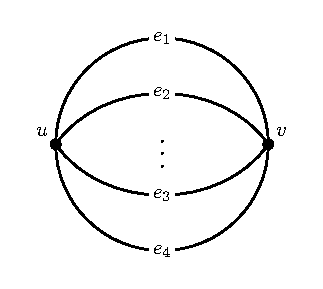
\includegraphics[width=0.32\textwidth]{figures/fig_bundle.pdf}
  \caption{A common-theta bundle of four full propagators. The vertices $u$ and $v$ carry no external
  legs, and every propagator $e_1,\ldots,e_4$ joins this same pair of vertices, hence the same pair of
  current components at every stage of the reduction. All four propagators therefore carry the identical
  theta argument $\Delta=\tau_u-\tau_v$ and form one bundle $\cB$ with $|\cB|=4$. The two vertices
  sit at the left and the right end, the outer two propagators make up the halves of one circle, and the
  vertical dots between the inner two propagators stand for any number of further propagators joining the same
  pair, so the bundle is not restricted to the four propagators drawn.}
  \label{fig:bundle}
\end{figure}

For each propagator $e$ of the bundle, write $\alpha_e$ for the coefficient of
$\theta(\Delta)$ and $\beta_e$ for the coefficient of $\theta(-\Delta)$.
\begin{enumerate}
  \item \emph{Multiply the thetas out first.} Since inside a bundle all thetas are the same
        function, $\theta(\Delta)^2=\theta(\Delta)$ and $\theta(\Delta)\theta(-\Delta)=0$, the
        product of $|\cB|$ propagators collapses to \emph{two} terms rather than $2^{|\cB|}$,
        \begin{equation}
          \prod_{e\in\cB}\Big(\theta(\Delta)\alpha_e+\theta(-\Delta)\beta_e\Big)
          =\theta(\Delta)\prod_{e\in\cB}\alpha_e
          +\theta(-\Delta)\prod_{e\in\cB}\beta_e .
          \label{eq:bundle-two-terms}
        \end{equation}
  \item \emph{One theta, one delta.} Differentiating the shared theta --- and only the theta, the two
        coefficients being left as spectators --- yields a single
        $\delta(\Delta)$ whose coefficient is the antisymmetric difference under
        $\alpha\leftrightarrow\beta$,
        $\big(\partial_\Delta\theta(\Delta)\big)\prod_{e\in\cB}\alpha_e
        +\big(\partial_\Delta\theta(-\Delta)\big)\prod_{e\in\cB}\beta_e
        =\delta(\Delta)\big(\prod_{e\in\cB}\alpha_e-\prod_{e\in\cB}\beta_e\big)$, so all contact information of
        the bundle is concentrated in one distribution and the two vertices are forced to coincide
        only once. The terms in which the derivative acts on $\alpha_e$ or $\beta_e$ instead are not
        contact terms: they are the regular part of the derivative, already carried by the
        $\text{M}_1$ generators of Sec.~\ref{sec:ibp}, and they do not merge any component
        (App.~\ref{app:theta}).
  \item \emph{Split and change basis.} Telescoping the antisymmetric difference and then collecting
        in $\mathsf d_e=\alpha_e-\beta_e$ and $\mathsf m_e=(\alpha_e+\beta_e)/2$ leaves only terms
        with an odd number of $\mathsf d$ factors, each with a numerical coefficient,
        \begin{equation}
          \prod_{e\in\cB}\alpha_e-\prod_{e\in\cB}\beta_e
          =\sum_{\substack{\varnothing\neq S\subseteq\cB\\|S|\ \mathrm{odd}}}
          2^{1-|S|}\prod_{e\in S}\mathsf d_e\prod_{e\notin S}\mathsf m_e .
          \label{eq:bundle-odd-subsets}
        \end{equation}
  \item \emph{Read off the events.} Every non-empty odd subset $S$ is one simultaneous contact
        event: the propagators of $S$ are contracted at once, their two vertices merge once, the component
        count drops by one, and the base power of the merged component follows
        \eqref{eq:base-power} with $|C|-1$ merge terms. The injection matrix
        $C^{(v,1)}_{st}$ of \eqref{eq:contact-injection} for such an event is the tensor product of
        the local selectors of the propagators in $S$, multiplied by $2^{1-|S|}$ and by the spectator
        factors $\mathsf m_e$.
\end{enumerate}
The package uses the collected form \eqref{eq:bundle-odd-subsets} rather than the telescoping sum term
by term, because enumerating the terms one by one would count the same sector transition
several times; the argument, the parity proof and the treatment of unselected propagators whose two vertices
become coincident are given in App.~\ref{app:theta}. The same symmetric part governs the boundary data of
a coincident propagator: Sec.~\ref{sec:boundary} explains why the two branch arrangements of one merged
propagator are replaced by their mean there, one mean per merged propagator.



\section{Using the package}
\label{sec:usage}

\subsection{Installation and loading}
\label{sec:overview}

This subsection collects the system requirements and the loading commands.

\paragraph{System requirements.}
\begin{itemize}
  \item A Wolfram Language kernel: Mathematica or the free Wolfram Engine (the package is a
        \texttt{.wl} package; no external Wolfram libraries are needed).
  \item Python 3.10 or newer with \texttt{python-flint>=0.6} and \texttt{sympy>=1.12} installed, for the numerical backend.
        \texttt{MadStree} follows a zero-probe policy: the interpreter is selected only by the explicit
        \texttt{PythonExecutable} option or, when that is \texttt{Automatic} (the default), by the
        \texttt{MADSTREE\_PYTHON} environment variable, falling back to \texttt{"python"}.
\end{itemize}
Install the dependencies in the Python interpreter used for numerical evaluation:
\begin{verbatim}
python -m pip install "python-flint>=0.6" "sympy>=1.12"
\end{verbatim}
Here \texttt{python} should be replaced by the selected interpreter if necessary.
No further backend installation is needed: \texttt{MadStree} bundles \texttt{FlintNDE}, a solver for first-order
matrix differential equations built on the exact ball arithmetic of \texttt{python-flint}, under
\texttt{MadStree/Vendor/FlintNDE}, and delegates every numerical task of this package to this
bundled copy. Its role in the numerical workflow is described in Sec.~\ref{sec:backend}.

\paragraph{Loading the package.}

Download or clone the official release repository
\url{https://github.com/J7C/dSIBP-Packages} and
set \texttt{madStreeDirectory} to the \texttt{MadStree} directory in the local repository,
add it to \texttt{\$Path}, and load with \texttt{Needs}:
\begin{verbatim}
madStreeDirectory = ".../dSIBP-Packages/MadStree";
AppendTo[$Path, madStreeDirectory];
Needs["MadStree`"];
\end{verbatim}
Replace the example path with the absolute path to the local \texttt{MadStree} directory.
This loads \texttt{MadStree.m}, which loads \texttt{Kernel/MadStree.wl} with explicit UTF-8.
Equivalently, load the kernel file directly:
\begin{verbatim}
Get[FileNameJoin[{madStreeDirectory, "Kernel", "MadStree.wl"}],
  CharacterEncoding -> "UTF-8"];
\end{verbatim}
Loading through \texttt{Needs} requires no user encoding option.
\texttt{MadStree} uses its bundled \texttt{FlintNDE} backend without requiring \texttt{Needs["FlintNDE`"]}.
Use a fresh kernel when switching versions, since \texttt{Needs} does not reload
an already loaded package.

After loading, \texttt{MSFlintNDEConfiguration[]} returns an association whose \texttt{"version"}
entry should be \texttt{"1.0"} and whose \texttt{"availableQ"} entry should be \texttt{True}. The
second value confirms that \texttt{flintnde/\_\_init\_\_.py} exists under the configured backend
directory, which is \texttt{Vendor/FlintNDE} relative to \texttt{madStreeDirectory} by default.
\begin{verbatim}
MSFlintNDEConfiguration[]["version"]
\end{verbatim}
\begin{verbatim}
MSFlintNDEConfiguration[]["availableQ"]
\end{verbatim}

\subsection{Input formats and core functions}
\label{sec:inputs}

\paragraph{Tree diagrams: \texttt{MSInitTree}.}

A tree is given by an association of vertices and propagators. The propagator list sits under
the input key \texttt{"lines"}, but we call these objects propagators throughout. A tree with two vertices and one massless propagator between them:
\begin{verbatim}
spec = <|
  "name" -> "masslessFullEdge",
  "vertices" -> {
    <|"id" -> v1, "externalLegEnergy" -> k1,
      "timePower" -> a1, "vertexType" -> "+"|>,
    <|"id" -> v2, "externalLegEnergy" -> k2,
      "timePower" -> a2, "vertexType" -> "+"|>
  },
  "lines" -> {
    <|"type" -> "massless", "endpoints" -> {v1, v2},
      "momentum" -> q, "nu" -> 1/2|>
  }
|>;
context = MSInitTree[spec];
\end{verbatim}
Vertex fields:
\begin{center}
\begin{tabular}{@{}lp{5.5cm}p{3.8cm}@{}}
\toprule
field & meaning & note\\
\midrule
\texttt{id} & vertex symbol & required\\
\texttt{externalLegEnergy} & external energy parameter (e.g.\ \texttt{k1}) & optional; default $0$\\
\texttt{timePower} & time-power variable $a_v$ (e.g.\ \texttt{a1}) & required\\
\texttt{vertexType} & contour assignment \texttt{"+"} or \texttt{"-"} & required\\
\bottomrule
\end{tabular}
\end{center}
Propagator fields:
\begin{center}
\begin{tabular}{@{}p{4.4cm}p{5.3cm}p{3.8cm}@{}}
\toprule
field & meaning & note\\
\midrule
\texttt{type} & \texttt{"massive"} or \texttt{"massless"} & required\\
\texttt{endpoints} & list of one external or two internal vertices & required\\
\texttt{momentum} & momentum variable $k_i$ (e.g.\ \texttt{q}) & required\\
\texttt{nu} & supplied Bessel/Hankel order $\nu$ & required for massive propagators; massless default $1/2$\\
\bottomrule
\end{tabular}
\end{center}
A massless propagator joining two internal vertices is classified internally as \texttt{masslessFull} and
always uses the shared mode-function two-state quotient basis of Sec.~\ref{sec:dlog}; there is no field that
selects another massless representation.
The initialization option \texttt{NuConvention} takes \texttt{"Positive"} (default) or
\texttt{"Negative"} and chooses the prefactor sign of $h(\nu,0;z)=z^{\pm\nu}H_\nu(z)$ introduced in
Sec.~\ref{sec:conventions}; it is fixed for the whole context and cannot be changed per call.

Propagator numbers are assigned from the input order. The Full, Cross or External class and the contour signs are derived from the \texttt{vertexType} of the two vertices the propagator joins; they are not supplied as a type value or as separate sign fields. A \texttt{"+"} vertex has phase $e^{-\ii E\tau}$ and a \texttt{"-"} vertex has phase $e^{+\ii E\tau}$, where $E$ is \texttt{externalLegEnergy}. An omitted or zero external energy is represented internally by an auxiliary variable whose target value is zero. Full propagators that join the same pair of vertices are grouped into one common-theta bundle automatically; the optional top-level field \texttt{"thetaBundles"} pins such a group explicitly as a list of propagator ids, and any group whose members do not join the same pair of vertices is rejected.
\paragraph{Loop diagrams without loop integral: \texttt{MSInitTimeGraph}.}

For a pure time-order graph the vertex and propagator fields are the same, but the graph may contain
cycles. A triangle cycle reads
\begin{verbatim}
cycleContext = MSInitTimeGraph[<|
  "vertices" -> {
    <|"id" -> t1, "externalLegEnergy" -> k1,
      "timePower" -> a1, "vertexType" -> "+"|>,
    <|"id" -> t2, "externalLegEnergy" -> k2,
      "timePower" -> a2, "vertexType" -> "+"|>,
    <|"id" -> t3, "externalLegEnergy" -> k3,
      "timePower" -> a3, "vertexType" -> "+"|>
  },
  "lines" -> {
    <|"type" -> "massless", "endpoints" -> {t1, t2},
      "momentum" -> q12, "nu" -> 1/2|>,
    <|"type" -> "massless", "endpoints" -> {t2, t3},
      "momentum" -> q23, "nu" -> 1/2|>,
    <|"type" -> "massless", "endpoints" -> {t3, t1},
      "momentum" -> q31, "nu" -> 1/2|>
  }
|>];
\end{verbatim}
Here every propagator joins two internal vertices, so all three are classified internally as
\texttt{masslessFull}. Once one of them is contracted, the remaining two connect the same pair of
components and therefore form the common-theta bundle of Sec.~\ref{sec:common-theta}.

\paragraph{Single-vertex integral families: \texttt{MSInitVertexFamily}.}

A single vertex needs no graph input. The compact input follows the reference
\texttt{ki/nui} convention,
\begin{verbatim}
vertexContext = MSInitVertexFamily[<|
  "ki" -> {k0, k1, k2},
  "nui" -> {a0, nu1, nu2},
  "hankelBranches" -> {1, 2}
|>, NuConvention -> "Positive"];
\end{verbatim}
where \texttt{First[ki]} is the pure vertex phase energy and \texttt{First[nui]} the base power of
$(-\tau)$; the remaining entries give, position by position, the $h$-block momenta and their Hankel
orders $\nu$, which are used exactly as in Sec.~\ref{sec:conventions}. The explicit alternative
\texttt{externalLegEnergy/timePower/hBlocks/exponentialBlocks} is also accepted, where each
$h$-block is an association with the keys \texttt{momentum}, \texttt{nu} and
\texttt{hankelBranch}. In contrast to the tree and time-graph functions, \texttt{MSInitVertexFamily} rejects any
field outside its own key set.

\paragraph{Package conventions.}
\label{sec:package}

The package implements the $h$ mode-function states of \eqref{eq:h-definition} with $z=-k\tau$ and the
single function name $h$, using
\begin{equation}
  h(\nu,0;z)=z^{\pm\nu}H_\nu(z),
  \label{eq:positive-order-h}
\end{equation}
where the plus sign is the default (\texttt{NuConvention->"Positive"}) and the minus sign gives
the convention of \cite{Chen:2023iix}; the two bases are related by $\nu\to-\nu$
(Sec.~\ref{sec:conventions}). The master integrals are the
$\text{I}_s(\bm 0;\bm a)$ of \eqref{eq:master-vector}, which on a single vertex is the one-vertex
family $\text{I}^{(0)}_{\tilde{\bm a};s_1\cdots s_n}$ of \eqref{eq:vertex-integral-family}; for
multi-vertex correlators they are the products and
sub-sector integrals of Sec.~\ref{sec:dlog}. Each master integral is represented by
\texttt{MSIntegral[sectorKey, aShifts, stateBits]}: \texttt{sectorKey} is a binary string over
the root propagators in the input order, with \texttt{"1"} for an uncontracted propagator and
\texttt{"0"} for a propagator contracted by a contact; \texttt{aShifts} assigns one integer shift of
the base time power to every vertex component, where a component is a maximal set of vertices
merged by the contractions; \texttt{stateBits} gives the mode-function state of every two-state slot of the
sector, in slot order. The connection of the masters
is the d log-form \eqref{eq:ndlogDE} of Sec.~\ref{sec:dlog}.

We give a few examples of \texttt{MSIntegral[sectorKey, aShifts, stateBits]}. For the three-vertex chain $v_1$--$v_2$--$v_3$ with internal propagators $l_{12}$, $l_{23}$, vertex
energies $k_1,k_2,k_3$ and time powers $a_1,a_2,a_3$, the contact-reachable sectors are the four
strings \texttt{"11"}, \texttt{"01"}, \texttt{"10"}, \texttt{"00"},
\begin{center}
\emph{(i) both propagators massive: $l_{12}$ with $\nu_{12}$, $l_{23}$ with $\nu_{23}$.}\\[2pt]
\footnotesize\begin{tabular}{@{}lllp{5.8cm}@{}}
\toprule
\texttt{sectorKey} & contracted & components & master integrals\\
\midrule
\texttt{"11"} & --- & $\{v_1\},\{v_2\},\{v_3\}$
  & \texttt{MSIntegral["11",\{0,0,0\},\{a,b,c,d\}]} (16)\\
\texttt{"01"} & $l_{12}$ & $\{v_1,v_2\},\{v_3\}$
  & \texttt{MSIntegral["01",\{0,0\},\{c,d\}]} (4)\\
\texttt{"10"} & $l_{23}$ & $\{v_1\},\{v_2,v_3\}$
  & \texttt{MSIntegral["10",\{0,0\},\{a,b\}]} (4)\\
\texttt{"00"} & $l_{12},l_{23}$ & $\{v_1,v_2,v_3\}$
  & \texttt{MSIntegral["00",\{0\},\{\}]} (1)\\
\bottomrule
\end{tabular}
\end{center}
\begin{center}
\emph{(ii) $l_{12}$ massive with $\nu_{12}$, $l_{23}$ massless.}\\[2pt]
\footnotesize\begin{tabular}{@{}lllp{5.8cm}@{}}
\toprule
\texttt{sectorKey} & contracted & components & master integrals\\
\midrule
\texttt{"11"} & --- & $\{v_1\},\{v_2\},\{v_3\}$
  & \texttt{MSIntegral["11",\{0,0,0\},\{a,b,r\}]} (8)\\
\texttt{"01"} & $l_{12}$ & $\{v_1,v_2\},\{v_3\}$
  & \texttt{MSIntegral["01",\{0,0\},\{r\}]} (2)\\
\texttt{"10"} & $l_{23}$ & $\{v_1\},\{v_2,v_3\}$
  & \texttt{MSIntegral["10",\{0,0\},\{a,b\}]} (4)\\
\texttt{"00"} & $l_{12},l_{23}$ & $\{v_1,v_2,v_3\}$
  & \texttt{MSIntegral["00",\{0\},\{\}]} (1)\\
\bottomrule
\end{tabular}
\end{center}
\begin{center}
\emph{(iii) both propagators massless.}\\[2pt]
\footnotesize\begin{tabular}{@{}lllp{5.8cm}@{}}
\toprule
\texttt{sectorKey} & contracted & components & master integrals\\
\midrule
\texttt{"11"} & --- & $\{v_1\},\{v_2\},\{v_3\}$
  & \texttt{MSIntegral["11",\{0,0,0\},\{r,s\}]} (4)\\
\texttt{"01"} & $l_{12}$ & $\{v_1,v_2\},\{v_3\}$
  & \texttt{MSIntegral["01",\{0,0\},\{r\}]} (2)\\
\texttt{"10"} & $l_{23}$ & $\{v_1\},\{v_2,v_3\}$
  & \texttt{MSIntegral["10",\{0,0\},\{r\}]} (2)\\
\texttt{"00"} & $l_{12},l_{23}$ & $\{v_1,v_2,v_3\}$
  & \texttt{MSIntegral["00",\{0\},\{\}]} (1)\\
\bottomrule
\end{tabular}
\end{center}


The vertex \texttt{vertexType} field (\texttt{"+"} or \texttt{"-"}) determines the sign of the pure
vertex exponential $e^{\ii k_0\tau}$ of \eqref{eq:vertex-integral-family}, and the pair of vertex types determines the SK class of each propagator, from which the default Hankel branches of
\eqref{eq:h-definition} follow; a propagator may override them with its own \texttt{hankelBranches}
field. The
package $h$ mode-function states are those of \eqref{eq:h-definition}, i.e.\
$h(\nu,1;z)=\partial_zh(\nu,0;z)$. \texttt{MSHTohMatrix} and \texttt{MShToHMatrix} give the local
$2\times2$ change of basis between the raw Hankel states and these states and its inverse, and
\texttt{MSConvertBasis} forms the corresponding Kronecker product over the slots of a sector, with the
massless shared mode-function two-state slot of Sec.~\ref{sec:massless} acting trivially on the reduced
mode-function states.



Once the context is initialized, the following functions expose the formula products of Sec.~\ref{sec:method}.

\paragraph{Core functions.}
\label{sec:core}

Most functions take the initialized \texttt{context};
\texttt{MSExportEvaluationData} takes a completed evaluation result instead.

\begin{center}
\begin{tabular}{@{}p{7.1cm}p{7.3cm}@{}}
\toprule
function & purpose\\
\midrule
\texttt{MSSectors[context]} & contact-reachable sectors in deterministic order (keys, contracted
propagators, master counts)\\
\texttt{MSMasterIntegrals[context]} & ordered master records; each \texttt{"integral"} field is an
\texttt{MSIntegral[sectorKey, aShifts, stateBits]}\\
\texttt{MSFormulaMatrices[context, key]} & per-component $\text{M}_1$, $\text{M}_0$ and energy letters $\kappa_{\bm a}$;
sector diagonalizer \texttt{"U"} and \texttt{"UInverse"}\\
\texttt{MSDLogDE[context]} & block-triangular d log-form potential $\Omega$, letters, certification
status\\
\texttt{MSReduce[expr, context]} & iterative IBP reduction to the master basis; scalar, list or nested table input\\
\texttt{MSContactMaps[context, key]} & parent-to-sub-sector contact maps\\
\texttt{MSWriteFormulaArtifacts[context]} & write formula products beside the caller\\
\texttt{MSFormulaData[context]} & aggregate all-sector masters, recurrence metadata and the d log-form DE\\
\texttt{MSEvaluatePath[context, pointSequence, opts]} & single-stage evaluation: boundary initialization and segment transport in one backend process; optional FlintNDE path planning\\
\texttt{MSReconstructEpSeries[context, ep, pointSequence, opts]} & Laurent series in the common analytic regulator: certified lowest power, automatic sample points, incremental fitting\\
\texttt{MSExportEvaluationData[evaluation, opts]} & export the saved ordinary-point records of an evaluation to CSV/JSON\\
\bottomrule
\end{tabular}
\end{center}

\begin{description}
  \item[\texttt{MSSectors[context]}] returns the sector list. Each sector key is the fixed-length
        bit string over the root propagators in input order (\texttt{"0"} contracted,
        \texttt{"1"} uncontracted); the
        sub-sector structure is discussed in Sec.~\ref{sec:dlog}. Keys are
        strings, not integers; leading zeros are part of the identity.
  \item[\texttt{MSMasterIntegrals[context]}] returns the ordered master records.
        Their \texttt{"integral"} fields contain the
        \texttt{MSIntegral[sectorKey, aShifts, stateBits]} objects of Sec.~\ref{sec:package}, i.e.\
        the master integrals $\text{I}_s(\bm 0;\bm a)$ of \eqref{eq:master-vector}.
        Use \texttt{Lookup[MSMasterIntegrals[context], "integral"]} to obtain this ordered basis.
        Each record also contains \texttt{"bareIntegral"}, \texttt{"normalization"} and
        \texttt{"definition"}. All matrices, boundary vectors and numerical results follow this order.
  \item[\texttt{MSFormulaMatrices[context, key]}] returns the component records under
        \texttt{"components"}, with fields \texttt{"M1"}, \texttt{"M0"} and
        \texttt{"energyLetters"} for the matrices and letters of Sec.~\ref{sec:global}.
        The sector diagonalizer of $\text{M}_0$ and its inverse are returned as
        \texttt{"U"} and \texttt{"UInverse"}; $\text{M}_1$ is already diagonal in the mode-function state basis.
        Here \texttt{key} is a sector-key string; omitting it, or passing \texttt{All},
        returns an association for all sectors. \texttt{MSContactMaps} accepts the same
        sector selection.
  \item[\texttt{MSDLogDE[context]}] returns \texttt{"omegaPotential"}, the matrix $\Omega$ of
        Sec.~\ref{sec:dlog} whose derivative along a path is the DE matrix, together with the
        letters (the arguments of the logarithms of \eqref{eq:omega-form}),
        \texttt{"letterMatrices"}, \texttt{"dlogResidual"}, \texttt{"constantResidueQ"} and the
        certification \texttt{"dlogStatus"}. Only the status \texttt{"certifiedByFormulaChecks"}
        certifies a closed d log-form, and only a certified potential may be used numerically.
  \item[\texttt{MSReduce[expr, context, MasterBasis -> Automatic]}] reduces finite linear
        combinations of legal \texttt{MSIntegral}s, or lists and nested tables of such
        expressions, by
        the lowering/raising recurrences $A_\pm$ of Sec.~\ref{sec:global} along the
        sub-sector structure of Sec.~\ref{sec:dlog}. Results include
        \texttt{"result"}, \texttt{"masterBasis"}, \texttt{"coefficientVector"},
        \texttt{"masterRules"},
        \texttt{"nonMasterResidual"}, \texttt{"remainingShiftedIntegrals"} and
        \texttt{"singularLayers"}; a full reduction requires a zero residual and an empty shifted
        list for every scalar expression. For list input, these fields preserve the input
        shape; \texttt{"elementResults"}, \texttt{"failurePositions"} and
        \texttt{"incompletePositions"} provide the element-level reports.
  \item[\texttt{MSFormulaData[context]}] returns all-sector masters, the per-sector
        $\text{M}_1/\text{M}_0/\text{T}_n$ recurrence metadata of Sec.~\ref{sec:global} and the complete
        block-triangular d log-form DE in the master order of \texttt{MSDLogDE};
        \texttt{TimePowerRules} may substitute the vertex time powers $a_i$ in the recurrence
        metadata, but the returned \texttt{"dlogDE"} remains analytic and unsubstituted.
  \item[\texttt{MSEvaluatePath[context, pointSequence, opts]}] is the single-stage numerical
        entry for evaluating the master integrals at the user points.
        \texttt{pointSequence} is a coordinate table in the format of Sec.~\ref{sec:numerics}.
        Fixed parameters are supplied once through \texttt{ParameterRules}. Boundary generation,
        transport and result records are described in Sec.~\ref{sec:numerics}; the principal
        options and point tags are summarized in Sec.~\ref{sec:options}.
  \item[\texttt{MSReconstructEpSeries[context, ep, pointSequence, opts]}] reconstructs the Laurent
        series of the master integrals in a common analytic regulator \texttt{ep}, with
        \texttt{MaximumEpPower} the highest returned power (default $0$, i.e.\ the pole terms and
        the finite part). It uses the same \texttt{pointSequence} and \texttt{ParameterRules}
        format as \texttt{MSEvaluatePath}. Only \texttt{ParameterRules}, not the coordinates,
        may depend on \texttt{ep}. By default, no \texttt{ep} values need to be supplied;
        \texttt{EpSamplePoints} and \texttt{EpValidationPoints} may instead specify the production
        points and disjoint validation points. The certificate conditions,
        sampling and fitting procedure are described in Sec.~\ref{sec:regulator}; the corresponding
        options are summarized in Sec.~\ref{sec:options}, and a complete application is
        presented in Sec.~\ref{sec:applications}.
  \item[\texttt{MSExportEvaluationData[evaluation, opts]}] exports the saved ordinary-point
        records of one \texttt{MSEvaluatePath} result, including the coordinates, the
        real/imaginary parts of every master, \texttt{"status"},
        \texttt{"relativeDifferenceInf"} and
        \texttt{"targetRelativeErrorMet"}, to CSV and JSON for downstream plotting tools; transient
        records are excluded. The two precision fields are the corresponding segment reports,
        not separate error estimates computed at every point. \texttt{ExportFormats} selects
        CSV, JSON or both, and \texttt{SignificantDigits} defaults to $16$;
        see Sec.~\ref{sec:outputs}.
\end{description}

\paragraph{Output organization.}
\label{sec:outputs}

\begin{itemize}
  \item Transient request JSON and backend logs:
        \texttt{results\_temp/\allowbreak nde/} beside the caller by default.
        Request and log files are deleted after a successful run and retained for backend
        failures; the package also deletes them for the structured \texttt{"singularPathRefused"}
        and \texttt{"leadingOrderRefused"} outcomes, which are results rather than failures.
        Successful JSON results remain in \texttt{results\_temp/\allowbreak cache/} for reuse.
        \texttt{MSRuntimeDirectory} may specify a different runtime directory.
  \item Saved point records: \texttt{MSEvaluatePath} returns the records under
        \texttt{"pointResults"}. An ordinary untagged coordinate row has
        \texttt{"status" -> "saved"}; \texttt{"saved"} is a status value, not a top-level key.
        A row \texttt{\{\{values...\}, "tmp"\}} gives a transient waypoint, represented by
        \texttt{"status" -> "transient"} and excluded from export.
        Singular-point classifications are returned under \texttt{"singularityClassifications"}
        by the same backend evaluation run.
  \item Formula artifacts: \texttt{MSWriteFormulaArtifacts[context]} writes \texttt{masters.wl},
        \texttt{recurrence\_metadata.wl}, \texttt{dlog\_de.wl} and \texttt{manifest.wl} to
        \texttt{results/\allowbreak madstree\_formula/\allowbreak run-UUID/} by default.
        \texttt{MSEvaluatePath} and \texttt{MSReconstructEpSeries} automatically write or reuse
        these analytic files before numerical transport and return their paths under
        \texttt{"formulaArtifacts"}.
  \item Evaluation export: \texttt{MSExportEvaluationData[result, MSOutputDirectory -> ...]} writes
        \texttt{evaluation\_data.csv} and \texttt{evaluation\_data.json} under
        the caller-chosen output directory (default
        \texttt{results/\allowbreak madstree\_evaluation/\allowbreak run-UUID/}), for downstream
        plotting tools.
  \item Cache identity: a successful-result cache key includes the request and the SHA-256
        identities of the backend adapter, the configured backend's \texttt{pyproject.toml}
        and sorted \texttt{flintnde/*.py}, so
        in-place source fixes invalidate stale cache entries automatically.
\end{itemize}
The package source directory never receives run artifacts.


\subsection{Numerical evaluation}
\label{sec:numerics}

With an initialized context, numerical evaluation proceeds in two steps: boundary generation and
transport. The workflow is single-stage: \texttt{MSEvaluatePath} partitions the user point
sequence into maximal consecutive complex-affine one-variable segments, pulls the d log-form
connection back once per segment, and sends all segments, the exact boundary conditions and the
user options to \texttt{FlintNDE} in one UTF-8 JSON request. With the default
\texttt{FlintNDEPathPlanning -> True}, \texttt{FlintNDE} plans the transport nodes inside each segment and
evaluates user points by fast multipoint evaluation; with \texttt{False} it uses every supplied
point as a node in input order, without inserting, removing, or replanning points. The bundled
backend is a synchronized copy of the standalone \texttt{FlintNDE} package released in the same
repository; its mechanisms are described below. \texttt{MSBoundaryData} and \texttt{MSEvaluatePath}
default to 200 decimal working digits; an explicit \texttt{WorkingPrecision} overrides the
default.

\paragraph{Boundary generation.}

\begin{verbatim}
targetRules = {k1 -> 9 I, k2 -> 3 I, q -> 1, a1 -> 1, a2 -> 1};

certificate = MSBoundaryChartCertificate[context, targetRules,
  RankOrder -> All];

boundary = MSBoundaryData[context, targetRules,
  BoundaryScale -> 4, WorkingPrecision -> 200];
\end{verbatim}
\texttt{MSBoundaryChartCertificate} verifies the nested blow-up chart of Sec.~\ref{sec:boundary}
(normal crossing, theta fixing, quotient checks) for the chosen strict energy rank;
\texttt{RankOrder -> All} checks every strict chart. \texttt{MSBoundaryData} consumes the
certificate and returns the leading Frobenius data at the $K_v\to\infty$ boundary. For every master
whose leading weight does not vanish, it returns one branch record with the Frobenius exponent, the
overall coefficient and the normalized leading vector, together with the anchor rules, the rank order
and the certificate itself.
If the chart is not certified, it returns \texttt{BoundaryChartNotCertified} and does not proceed
to numerics. The energies in the example are positive imaginary so that the vertex factors
$e^{-\ii E\tau}$ damp at $\tau\to-\infty$; the rank order of the boundary is derived from the
supplied target point, largest damping energy first, unless \texttt{RankOrder} fixes it.

\paragraph{Transport.}

\begin{verbatim}
pointSequence = {{k1, k2}, {9 I, 3 I}};
parameterRules = {q -> 1, a1 -> 1, a2 -> 1};

result = MSEvaluatePath[context, pointSequence,
  ParameterRules -> parameterRules,
  BoundaryScale -> 4, RankOrder -> {v1, v2},
  WorkingPrecision -> 200, TransportOrder -> 80,
  ReferenceTransportOrder -> 104,
  TargetRelativeError -> "1e-20",
  MessageLanguage -> "EN"];

result["pointResults"]
\end{verbatim}
The second argument is the \emph{point sequence}: its first row lists the movable coordinate
symbols, and every further row supplies one numerical value for each of them, in the same order.
The remaining symbols of the target point, here \texttt{q}, \texttt{a1} and \texttt{a2}, are fixed
once for the whole run through \texttt{ParameterRules}. For several target points, append one row per
point,
\begin{verbatim}
pointSequence = {{k1, k2}, {8 I, 2 I}, {7 I, 4 I}, {6 I, 5 I}};
\end{verbatim}
and \texttt{MadStree} groups the
points into maximal consecutive complex-affine segments and pulls each segment back once, while
\texttt{FlintNDE} evaluates every point in one process, including the extra points inside a node's
convergence disk, without changing the path. For a single-vertex integral family, run the same
single-stage entry on the vertex context. The principal transport options and the point tags are
summarized in Sec.~\ref{sec:options}. If every d log-form letter is constant on a segment, every
pulled-back derivative vanishes; the segment is then a zero connection with no finite poles and
transport proceeds as for any ordinary segment.

\paragraph{Reading the result.}

\texttt{result} is an association whose \texttt{"pointResults"} entry is the list of point records.
Every saved ordinary point carries
\texttt{"coordinate"}, \texttt{"value"} (the master vector in master order), \texttt{"status"}
(equal to
\texttt{"saved"} for ordinary points) and \texttt{"userIndex"}; transient \texttt{"tmp"} points
are used only as intermediate points of the path. The current version does not provide leading-order
point labels: every tag other than \texttt{"tmp"} is rejected. A user chain that
crosses a pole or leaves a local convergence disk fails closed; the two options that decide this,
\texttt{SingularityMode} and \texttt{FlintNDEPathPlanning}, are described in
Sec.~\ref{sec:options}. The exported per-point
\texttt{"relativeDifferenceInf"} and \texttt{"targetRelativeErrorMet"} are obtained from the
truncation certification of Sec.~\ref{sec:backend}.
A way to read a saved value that does not depend on the path is
\begin{verbatim}
savedPoints = Select[result["pointResults"], #["status"] === "saved" &];
firstPoint = First[savedPoints];
firstPoint["value"]
\end{verbatim}

\paragraph{The numerical backend.}
\label{sec:backend}

\texttt{FlintNDE} solves first-order matrix differential equations with exact
$Q(\ii)(s)$-coefficient systems; \texttt{MadStree} embeds a synchronized copy and
feeds it only single-variable pullbacks of the d log-form connection. Three mechanisms are responsible
for the current performance:
\begin{itemize}
  \item \emph{Pole--residue transport.} An ordinary segment is serialized as its pole--residue
        representation $A(x)=P(x)+\sum_jR_j/(x-p_j)$, with $P$ of arbitrary degree and the residues
        $R_j$ of coincident letters merged. The backend generates the solution Taylor coefficients
        by a recurrence that carries one auxiliary state vector per pole, avoiding the Cauchy sampling
        and discrete-Fourier coefficient reconstruction of a generic analytic-matrix backend.
  \item \emph{Embedded truncation certification.} The backend is always called in its embedded
        certification mode, which runs one chain at \texttt{ReferenceTransportOrder} and takes the
        primary result from the coefficient prefix truncated at \texttt{TransportOrder}, re-evaluated
        by Horner's rule. The per-segment truncation difference is returned as a local error estimate,
        so the \texttt{"relativeDifferenceInf"} and \texttt{"targetRelativeErrorMet"} fields remain
        available without the cost of a second chain. The call is upgraded to independent primary and
        reference chains whenever the prefix cannot carry the certification: on a multi-segment path,
        on a path with singular local data, for a run that starts from Frobenius boundary data, and
        for a request with saved points.
  \item \emph{Fast multipoint evaluation.} With \texttt{FlintNDEPathPlanning -> True}, \texttt{FlintNDE}
        plans nodes inside each segment; user points covered by one expansion node form an
        evaluation bucket and are evaluated from the cached vector series. Buckets with at least
        eight points use the subproduct/remainder tree of fast multipoint evaluation, and small
        buckets use a simple iterative algorithm to avoid the overhead of the tree. User points in the same
        complex-affine segment $x(s)=x_0+s\,v$ share node coefficients whenever they lie in the same
        convergence disk; different segments never share local coefficients.
\end{itemize}
Singularity handling is explicit: the default \texttt{SingularityMode -> "Automatic"} maps to the
backend jump mode, so a segment that meets a supported singularity is crossed by an explicit
local-basis jump instead of being refused or detoured. The three modes and their interaction with
\texttt{FlintNDEPathPlanning} are listed in Sec.~\ref{sec:options}. Exact Lee--Moser balances,
strictly decoupled exponential times, and power-log recurrences are handled, while resonances
whose local bases cannot be constructed, and any ramification or general Stokes requirement, fail
closed. The internal working bits are $\lceil\mathrm{WP}\log_2 10\rceil+32$, where WP is the value of
\texttt{WorkingPrecision} in decimal digits, and all path geometry (segment
projections, match ratios, rotation factors, winding/monodromy) is kept in Arb/Acb precision.
If the backend rewrites the problem in real variables, so that $k=-\ii\kappa$, then $-k^2=+\kappa^2$;
a program token named \texttt{ik} then denotes the real variable $\kappa$, and \texttt{ik\^{}2} is its
square, not the imaginary unit times $k^2$.

\subsection{Laurent-series reconstruction}
\label{sec:regulator}

When all vertex time powers share a common analytic regulator $\varepsilon$, e.g.\
$a_v=1+\varepsilon$, the master integrals develop a Laurent series
\begin{equation}
  I(\varepsilon)=\sum_{p=n_{\min}}^{m}c_p\,\varepsilon^p
  +O(\varepsilon^{m+1}),
  \label{eq:regulator-laurent}
\end{equation}
and \texttt{MSReconstructEpSeries[context, ep, pointSequence, MaximumEpPower -> m]}
reconstructs the coefficients $c_{n_{\min}},\ldots,c_m$. The user supplies no
$\varepsilon$ values; the lowest power is not a numerical fit parameter.

This procedure follows the one used by AMFlow \cite{Liu:2022chg,Huang:2026rjb}. The transport
is numerical, while the regulator dependence of the result has to stay analytic, and carrying that
analytic dependence through every matrix multiplication of a long path would dominate the cost.
Each sample point is therefore evaluated numerically at a fixed value of $\varepsilon$, and the
coefficients of \eqref{eq:regulator-laurent} are recovered afterwards from the final values of all
runs, which is what keeps a multi-order expansion affordable.

\paragraph{Certification of the lowest power.}
Before any numerical solve at nonzero $\varepsilon$, \texttt{MadStree} constructs a support
certificate from the symbolic boundary conditions and the d log-form DE of the production
context. It requires:
\begin{enumerate}
  \item regulator-independent path coordinates and no negative Laurent power at
        $\varepsilon=0$ in any d log-form matrix, pulled-back connection, or residue;
  \item finite-Laurent boundary branches, where branches with the same limiting Frobenius
        exponent and log degree are first combined with their physical weights and leading
        vectors, and only then are the component valuations of the record field
        \texttt{"componentValuations"} extracted;
  \item at least one provably nonzero coefficient at the lowest power of the combined
        boundary; a noninteger power, non-Laurent structure, undecidable coefficient, or
        support entirely above the requested user range fails closed.
\end{enumerate}
For $n_{\min}<0$ the certificate describes a finite meromorphic Laurent boundary, not an
analytic boundary at $\varepsilon=0$; analyticity is recorded only when $n_{\min}\geq0$.
Along the current finite path an $\varepsilon$-analytic invertible fundamental matrix
preserves the valuation of nonzero formal boundary conditions, so the certified $n_{\min}$ is
passed directly to the sampling plan. A rank drop of an individual Frobenius recurrence
operator at $\varepsilon=0$ is retained as a resonance diagnostic only; it is not by itself
interpreted as a $1/\varepsilon$ pole of the already combined physical boundary.

\paragraph{Sampling, fitting and validation.}
Given the highest requested power $m$ and the certified lowest power $n_{\min}$, the plan sets
\begin{equation}
  P=\max(0,-n_{\min}),\qquad
  \Delta=m-n_{\min},\qquad
  N_{\rm fit}=\max\!\left(\left\lceil\tfrac52\Delta+P\right\rceil,\Delta+1+f\right),
  \label{eq:regulator-fit-count}
\end{equation}
where $f=\texttt{EpFitExtraOrder}$, default $2$, is the number of powers the fit keeps above the
user maximum: the second term in the maximum in \eqref{eq:regulator-fit-count} would be $\Delta+1$ if
only $c_{n_{\min}},\ldots,c_m$ were fitted, and the extra $f$ is what makes the interpolation reach
past $c_m$ in every run. A user-supplied pool \texttt{EpSamplePoints} and the refit rounds below may
raise $N_{\rm fit}$ further, but $N_{\rm fit}$ is never below $\Delta+1$.
The plan then chooses the $\varepsilon$ scale and precisions
\begin{equation}
  \alpha_\varepsilon=\frac{P}{4}+\frac{g}{\Delta+1},\qquad
  \varepsilon_0=10^{-\alpha_\varepsilon},\qquad
  p_0=\max\!\left(\left\lceil(N_{\rm fit}+P)\alpha_\varepsilon\right\rceil,30\right),
  \label{eq:regulator-scale-precision}
\end{equation}
where $g=\texttt{EpGoalDigits}$ is the requested decimal accuracy. The working precision is
$\max(200,\lceil2(1+e)p_0\rceil)$ with $e$ the extra-precision fraction; the primary
transport order is $4p_0$ and the reference chain adds
$\lceil\max(50,p_0/5)\rceil$ orders. All $N_{\rm fit}$ production points enter one square
Acb Vandermonde system with powers up to $\varepsilon^{n_{\min}+N_{\rm fit}-1}$; only
$c_{n_{\min}},\ldots,c_m$ are returned, and no least squares or pseudoinverse is used.
Independent validation points are placed at a fixed fraction of the production scale, never
enter the fit, and at each of them the fitted series, summed over all $N_{\rm fit}$ internal powers up
to $n_{\min}+N_{\rm fit}-1$ and hence including the buffer powers above the requested maximum $m$, must
reproduce the directly transported value to the relative tolerance $10^{-g}$; otherwise
the run fails closed. What such a residual certifies is the fit against that tolerance, not a number of
correct digits of the returned coefficients $c_{n_{\min}},\ldots,c_m$; those are carried and reported at
the working precision above.

\paragraph{Incremental expansion and parallelism.}
The initial fit includes at least two powers above the user maximum
(\texttt{EpFitExtraOrder -> 2}). If validation fails, each subsequent round adds
\texttt{EpFitOrderIncrement -> 2} powers, solves only the new production points, and reuses
every previous production and validation value, for at most \texttt{EpFitMaximumRounds -> 3}
rounds; the tolerance is not relaxed and the caches are not discarded. Independent
$\varepsilon$ tasks run in an outer process pool bounded by \texttt{ParallelTaskCount -> 12},
whose effective concurrency is the smaller of the limit and the number of tasks; this is
separate from the in-process \texttt{ctx.threads} of \texttt{python-flint}.
The third application example in Sec.~\ref{sec:applications} runs this procedure on a divergent
configuration.

\subsection{Options, validation and common pitfalls}
\label{sec:options}

The principal options of the numerical workflow are summarized below.
\begin{center}
\begin{tabular}{@{}p{5.0cm}p{9.3cm}@{}}
\toprule
option & meaning\\
\midrule
\texttt{FlintNDEPathPlanning} & \texttt{True} (default): \texttt{FlintNDE} plans nodes and uses fast
multipoint evaluation; \texttt{False}: user points as nodes in input order\\
\texttt{SingularityMode} & \texttt{"Automatic"} (default), \texttt{"Avoid"} or \texttt{"SingularityJump"}\\
\texttt{MessageLanguage} & \texttt{"EN"} (default) or \texttt{"CN"}, case-sensitive\\
\texttt{BoundaryScale} & scale setting the damping energies at the finite boundary anchor ($>1$; default 8)\\
\texttt{BoundarySeriesOrder} & boundary-order metadata and regulator recurrence diagnostics; not the numerical Frobenius start order in the present generic workflow\\
\texttt{RankOrder} & vertex order by damping energy $K_v$ (default \texttt{Automatic}: from the first target point)\\
\texttt{WorkingPrecision} & integer working precision in decimal digits, at least 20; default 200\\
\texttt{TransportOrder} / \texttt{ReferenceTransportOrder} & primary and reference local-series orders, including the numerical Frobenius start; defaults 48 and 64, with the reference order strictly larger\\
\texttt{TargetRelativeError} & target relative error of the primary/reference check; default \texttt{"1e-25"}\\
\texttt{MaximumEpPower} & highest returned regulator power of \texttt{MSReconstructEpSeries}
(default 0)\\
\texttt{EpGoalDigits} & requested decimal accuracy of the reconstructed regulator coefficients
(default 20)\\
\texttt{EpFitExtraOrder} / \texttt{EpFitOrderIncrement} / \texttt{EpFitMaximumRounds} & internal
buffer powers, per-round increment and maximum refit rounds of the regulator fit (defaults 2, 2, 3)\\
\texttt{ParallelTaskCount} & maximum concurrent \texttt{ep} backend processes in \texttt{MSReconstructEpSeries} (default 12)\\
\texttt{PythonExecutable} & Python command for the \texttt{FlintNDE} adapter (default \texttt{Automatic})\\
\texttt{MSRuntimeDirectory} & temporary-file root (default: \texttt{results\_temp} in the calling script or notebook directory)\\
\bottomrule
\end{tabular}
\end{center}

The transport orders and \texttt{TargetRelativeError} above apply to
\texttt{MSEvaluatePath}. For \texttt{MSReconstructEpSeries}, these three options
are not accepted; the numerical settings are planned from \texttt{EpGoalDigits}.
Its \texttt{BoundarySeriesOrder} defaults to \texttt{Automatic}, whereas
\texttt{MSEvaluatePath} uses 24.

The saved/transient distinction is not a transport option: it is a tag attached to the coordinate
rows below the symbol header, which are bare value lists or \texttt{\{\{values...\},"tmp"\}}.
With \texttt{SingularityMode -> "Avoid"}, interior singularity crossings are refused, and the
refusal names the interior singular points of the path. The default \texttt{"Automatic"} mode
allows supported singularity jumps when \texttt{FlintNDEPathPlanning -> True};
an explicit \texttt{"SingularityJump"} also requires this setting.
When planning is disabled, \texttt{"Automatic"} behaves as \texttt{"Avoid"}.
An explicitly requested
terminal singular point is handled by local classification and evaluation,
rather than by ordinary Taylor transport through the singularity.


Limitations and fail-closed guarantees:
\begin{itemize}
  \item No loop-momentum integration, no sampled IBP, no Kira or external reduction.
  \item \texttt{"dlogStatus"} must be \texttt{"certifiedByFormulaChecks"}; otherwise the DE is not
        consumed.
  \item Uncertified boundary charts and singular points beyond the
        backend's certified capabilities all fail closed; resonances whose local bases cannot be
        constructed return structured refusals, and ordinary Taylor transport is never used across
        singular points.
  \item An incomplete \texttt{MSReduce} call may return an association with
        \texttt{"status" -> "partiallyReduced"} or \texttt{"status" -> "failed"},
        rather than a top-level \texttt{Failure}. Inspect
        \texttt{"remainingShiftedIntegrals"} and \texttt{"nonMasterResidual"}.
  \item For \texttt{MSEvaluatePath}, check
        \texttt{result["flintNDE"]["targetRelativeErrorMet"]}, not only
        \texttt{result["status"]}. For \texttt{MSReconstructEpSeries}, check
        \texttt{"precisionTargetMet"}; coefficients may be returned with
        \texttt{"status" -> "computed\_with\_warning"} if the target is not met.
  \item The production boundary never uses defining integrals; finite-point defining integrals
        exist only inside independent validation programs.
\end{itemize}

\paragraph{Common pitfalls.}
\label{sec:pitfalls}

\begin{enumerate}
  \item \textbf{Convention}: \texttt{NuConvention} is chosen at initialization only
        (\texttt{"Positive"} by default). To compare with the formulas of
        \cite{Chen:2024glu}, initialize with \texttt{NuConvention -> "Negative"}, which selects
        the minus sign in \eqref{eq:positive-order-h}.
  \item \textbf{Sector keys}: fixed-length strings; leading zeros and the string type are part of
        the identity (Sec.~\ref{sec:dlog}).
  \item \textbf{Single-stage workflow}: call \texttt{MSEvaluatePath} directly. \texttt{MadStree} in this version does not
        provide \texttt{MSGeneratePath}, \texttt{MSEvaluatePlannedPath}, public plan objects, old JSON
        schemas or any migration wrapper.
  \item \textbf{Singularity handling}: the default is \texttt{SingularityMode -> "Automatic"},
        where \texttt{"Automatic"} is a string, not the symbol \texttt{Automatic}.
        Use \texttt{"Avoid"} to refuse interior crossings. Supported jumps require
        \texttt{FlintNDEPathPlanning -> True}, and the user must check the multivalued branch.
  \item \textbf{Point tags}: after the coordinate-symbol header, only bare value lists and
        \texttt{\{\{values...\},"tmp"\}} are accepted; every other tag, including
        \texttt{"lo"}, is rejected.
  \item \textbf{Backend environment}: \texttt{MadStree} follows the zero-probe policy of
        Sec.~\ref{sec:overview}, so the interpreter is the one selected there and must be able to
        import the embedded \texttt{flintnde}. Backend failures report captured output through
        messages such as \texttt{backendLaunchFailed} and \texttt{backendRunFailed}; retained runtime
        logs contain the details. After a successful call, and after a structured refusal of a
        singular path, the package removes the temporary input and log files.
  \item \textbf{Message language}: \texttt{MessageLanguage} accepts only \texttt{"EN"} and
        \texttt{"CN"} (case-sensitive), with \texttt{"EN"} the default.
  \item \textbf{Encoding}: loading through \texttt{Needs} uses explicit UTF-8 internally and needs
        no user encoding option; if loading the kernel file directly fails with syntax errors, set
        \texttt{\$CharacterEncoding = "UTF-8"} before loading.
\end{enumerate}

\section{Examples}
\label{sec:examples-section}

This section lists the examples distributed with the package and three applications computed
with them.
Sec.~\ref{sec:examples} describes the seven distributed examples, which exercise
recurrence reduction, single-vertex families, time-order charts, massless and massive trees,
zero external-leg energy, and the regulator reconstruction of Sec.~\ref{sec:regulator}.
Sec.~\ref{sec:applications} presents three numerical applications: the tree with three vertices and
two massive exchanges, whose transported results are compared with the multivariate hypergeometric
representation of \cite{Xianyu:2023ytd}; the bubble time kernel evaluated at fixed internal
momenta; and the massless three-vertex chain evaluated in the regulator mode, which demonstrates
the certified Laurent reconstruction of Sec.~\ref{sec:regulator} on a divergent configuration.
The comparisons underlying the verification tasks of Sec.~\ref{sec:verification} are not repeated
here. They cover the single-vertex families and the massive two-vertex correlator against
\cite{Chen:2024glu}, and the IBP relations and differential equations against the
\texttt{dSIBP} package~\cite{dSIBP:inPreparation}.

\subsection{Package examples}
\label{sec:examples}
Each example is a Wolfram Language script; together they exercise the complete workflow:
\begin{itemize}
  \item \texttt{01\_massless\_full\_edge.wl}: the massless shared mode-function two-state simplification of
        Sec.~\ref{sec:massless}, masters, recurrence, d log-form DE and the automatic
        boundary/numerical entry; it also demonstrates the
        single-stage multipoint workflow, with CSV/JSON export;
  \item \texttt{02\_single\_vertex\_family.wl}: single-vertex integral family input, local tensor
        inverses (Sec.~\ref{sec:global}), and finite-combination reduction;
  \item \texttt{03\_time\_only\_cycle\_chart.wl}: time-order cycle input, common-theta contacts
        (Sec.~\ref{sec:common-theta} and App.~\ref{app:theta}), and
        all strict-rank chart certificates; contacts are discussed in Sec.~\ref{sec:dlog};
  \item \texttt{04\_three\_vertex\_tree.wl}: a three-vertex, two-propagator massless tree
        ($+++$ vertex structure), following the same flow as example 01, with a single-stage
        multipoint evaluation and CSV/JSON export;
  \item \texttt{05\_massive\_three\_vertex\_tree.wl}: a three-vertex, two-propagator massive tree
        ($+++$ vertex structure) with non-half-integer \texttt{nu12=3/4}, \texttt{nu23=1/3},
        followed by a single-stage multipoint evaluation and CSV/JSON export;
  \item \texttt{06\_massless\_three\_vertex\_ep\_regularization.wl}: a three-vertex massless tree
        with the analytic regulator $a_1=-1+\varepsilon$, $a_2=a_3=1+\varepsilon$, whose
        $\varepsilon=0$ time integrals genuinely diverge; the user requests
        only the highest regulator power (\texttt{MaximumEpPower -> 0}), and the package
        certifies the lowest power $n_{\min}$ from the symbolic boundary and DE before any
        numerical solve (text below); its numerical
        reconstruction is presented as the third application in Sec.~\ref{sec:applications};
  \item \texttt{07\_zero\_external\_leg\_energy.wl}: zero external-leg energy, represented through an auxiliary energy with zero target value.
\end{itemize}

In Example~06, the vertex-1 unit $u_1=a_1+1$ equals $\varepsilon$, and every
factorized boundary weight that isolates this unit as a standalone factor carries a
$\Gamma(\varepsilon)$ simple pole, while the nine-dimensional DE has no negative $\varepsilon$
power. The certificate therefore gives $n_{\min}=-1$, decided by the combined
physical boundary and not by any individual resonance.

Each example ends with a failure gate: it prints \texttt{Example PASSED} and exits $0$ only when
every checked result is a non-\texttt{Failure} object, and exits $1$ with the reason otherwise.
Run them in a Mathematica front end section by section, or with
\begin{verbatim}
wolframscript -file .../Examples/01_massless_full_edge.wl
\end{verbatim}

\subsection{Application examples}
\label{sec:applications}
We illustrate the workflow of \texttt{MadStree} with three examples, using \texttt{FlintNDE}
for numerical transport. All timings measure elapsed time on a personal computer.

\paragraph{Tree with three vertices and two massive scalar exchanges}

The first example is the chain with three vertices in figure~\ref{fig:tree-diagram}.
\begin{figure}[H]
  \centering
  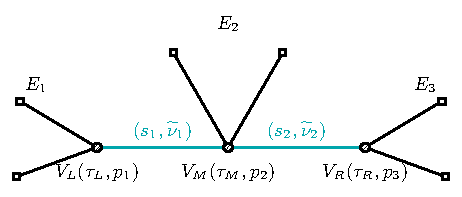
\includegraphics[width=0.72\textwidth]{figures/fig_tree_diagram.pdf}
  \caption{Tree with three vertices and two massive scalar propagators, drawn with the
  in-in Feynman rules of Sec.~\ref{sec:conventions} for the all-plus assignment
  $(+++)$: the time vertices are hatched circles on a horizontal axis, all on the
  \texttt{"+"} branch of the in-in contour, each carrying its conformal time $\tau_L$, $\tau_M$
  or $\tau_R$ and time power $p_1,p_2,p_3$ in the label $V_v(\tau_v,p_v)$ below it, together
  with a schematic fan of two external legs ending in open squares and labeled by the
  summed external energy $E_v=\sum_j k_{v,j}$. The internal propagators are drawn in teal
  and carry their momentum magnitudes and mass labels
  $(s_1,\widetilde\nu_1)$, $(s_2,\widetilde\nu_2)$ above the propagator.}
  \label{fig:tree-diagram}
\end{figure}

The vertices $L,M,R$ have conformal times $\tau_L,\tau_M,\tau_R$.
The two internal propagators connect $L$ to $M$ and $M$ to $R$, respectively.
Each vertex carries a fan of external legs; the momentum magnitudes $k_{v,j}$
of the legs at vertex $v$ sum to its external energy, $E_v=\sum_j k_{v,j}$.
The internal momentum magnitudes are $s_1,s_2$, and the Hankel orders are
$\nu_1,\nu_2$. For the masses in the principal series used here,
$\nu_i=\ii\widetilde\nu_i$, with real $\widetilde\nu_i$.
Each vertex has a contour sign $\sigma_v=\pm1$;
figure~\ref{fig:tree-diagram} is drawn for the all-plus assignment
$\sigma_L=\sigma_M=\sigma_R=+1$, and the assignments computed in this
application are fixed below.

From figure~\ref{fig:tree-diagram}, the function family of this example is built from one time
integration per vertex, carrying the time power $(-\tau_v)^{\nu_{0v}}$ and the external exponential
$e^{\ii\sigma_vE_v\tau_v}$, and from one propagator kernel per internal propagator, each kernel
carrying the mode-function states of its two endpoints. We first make these endpoint mode-function
states explicit:
\begin{equation}
 \begin{aligned}
 h^{(r)}(\nu,0;z)&=z^{-\nu}H^{(r)}_\nu(z),\\
 h^{(r)}(\nu,1;z)&=\partial_z h^{(r)}(\nu,0;z)
                  =-z^{-\nu}H^{(r)}_{\nu+1}(z),
 \qquad r=1,2.
 \end{aligned}
 \label{eq:application-endpoint-states}
\end{equation}
Here $r$ selects the Hankel function and the binary index selects the
undifferentiated or differentiated mode-function state. We use the same Hankel order
at both vertices of each propagator; constant factors from the physical mode
normalization are restored when forming the correlator.
To display the time ordering explicitly, define
\begin{equation}
 \begin{aligned}
 W_{>,\nu;ab}(s;\tau,\tau')
 &=h^{(1)}(\nu,a;-s\tau)h^{(2)}(\nu,b;-s\tau'),\\
 W_{<,\nu;ab}(s;\tau,\tau')
 &=h^{(2)}(\nu,a;-s\tau)h^{(1)}(\nu,b;-s\tau'),
 \qquad a,b\in\{0,1\}.
 \end{aligned}
 \label{eq:application-line-products}
\end{equation}
These two products are $G_>$ and $G_<$ of \eqref{eq:bulk-bulk-propagators} with the mode prefactors
removed and the two mode-function states made explicit. The propagator kernel of contour type
$\sigma\sigma'$, written $\mathcal G_{\sigma\sigma',\nu;ab}(s;\tau,\tau')$ below, is then the
time-ordered combination of the two products exactly as \eqref{eq:sk-propagators} combines $G_>$
and $G_<$: $\mathcal G_{++}$ and $\mathcal G_{--}$ take $\theta(\tau-\tau')W_{>}$ plus
$\theta(\tau'-\tau)W_{<}$ and $\theta(\tau-\tau')W_{<}$ plus $\theta(\tau'-\tau)W_{>}$, while
$\mathcal G_{+-}=W_{<,\nu;ab}$ and $\mathcal G_{-+}=W_{>,\nu;ab}$ carry no theta function. The binary
indices act only on the Hankel factors, never on the step functions, and every kernel has the
arguments $(s;\tau,\tau')$.

\emph{Convention remark.} This application uses the option
\texttt{NuConvention -> "Negative"}, i.e.\ $s_\nu=-1$ in the unified definition of
Sec.~\ref{sec:notation}, because the mode functions it starts from follow \cite{Chen:2024glu}, where
they are written with that option; \eqref{eq:application-endpoint-states} is therefore the $-\nu$
reading of \eqref{eq:h-definition}. This is not a third convention: the package default is
$s_\nu=+1$, with $h^{(r)}(\nu,0;z)=z^{+\nu}H^{(r)}_\nu(z)$ and
$h^{(r)}(\nu,1;z)=z^{+\nu}H^{(r)}_{\nu-1}(z)$, and the two readings are related by the single
simultaneous replacement $\nu\to-\nu$ of Sec.~\ref{sec:notation}, which must also be applied to the
effective time powers below.

For $\boldsymbol\sigma=(\sigma_L,\sigma_M,\sigma_R)$, the Top-sector master
integrals are
\begin{equation}
 \begin{aligned}
 \text{I}^{\boldsymbol\sigma}_{abcd}
 ={}&\int_{-\infty}^{0}d\tau_L\,d\tau_M\,d\tau_R\,
 (-\tau_L)^{\nu_{0L}}(-\tau_M)^{\nu_{0M}}(-\tau_R)^{\nu_{0R}}\\
 &\times e^{\ii(\sigma_LE_1\tau_L+\sigma_ME_2\tau_M+\sigma_RE_3\tau_R)}\\
 &\times\mathcal G_{\sigma_L\sigma_M,\nu_1;ab}(s_1;\tau_L,\tau_M)
 \mathcal G_{\sigma_M\sigma_R,\nu_2;cd}(s_2;\tau_M,\tau_R).
 \end{aligned}
 \label{eq:tree-indexed-masters}
\end{equation}
Here $a,b,c,d\in\{0,1\}$. Each time integral runs from $-\infty$ to $0$ with the Bunch--Davies
prescription. Each massive propagator carries one mode-function state at each of its two vertices,
two per propagator; the two propagators of this graph therefore carry four, and the indices
$a,b,c,d$ are the values of these four mode-function states, taken in the endpoint order
$(L_1,M_1,M_2,R_2)$. Thus the Top sector consists of the sixteen masters
\begin{equation}
 \begin{aligned}
 \bm{\text I}^{\boldsymbol\sigma}_{\mathrm{Top}}
 =\bigl(&\text{I}^{\boldsymbol\sigma}_{0000},
        \text{I}^{\boldsymbol\sigma}_{0001},
        \text{I}^{\boldsymbol\sigma}_{0010},
        \text{I}^{\boldsymbol\sigma}_{0011},
        \text{I}^{\boldsymbol\sigma}_{0100},
        \text{I}^{\boldsymbol\sigma}_{0101},
        \text{I}^{\boldsymbol\sigma}_{0110},
        \text{I}^{\boldsymbol\sigma}_{0111},\\
       &\text{I}^{\boldsymbol\sigma}_{1000},
        \text{I}^{\boldsymbol\sigma}_{1001},
        \text{I}^{\boldsymbol\sigma}_{1010},
        \text{I}^{\boldsymbol\sigma}_{1011},
        \text{I}^{\boldsymbol\sigma}_{1100},
        \text{I}^{\boldsymbol\sigma}_{1101},
        \text{I}^{\boldsymbol\sigma}_{1110},
        \text{I}^{\boldsymbol\sigma}_{1111}\bigr)^{\mathsf T},
 \end{aligned}
 \label{eq:tree-top-vector}
\end{equation}
one for each of the sixteen values of $(a,b,c,d)\in\{0,1\}^4$.
The entry $\text{I}^{\boldsymbol\sigma}_{0000}$ is the one with no
derivative acting on the mode-function states and no additional
integer shifts in the time powers. Equation \eqref{eq:tree-indexed-masters} is the sector
$\mathrm{Top}=(\xi_1\xi_2)=(11)$ of \eqref{eq:sector-key}, with $c_{\mathrm{Top}}=c_V=3$ components
by \eqref{eq:component-count} and $n^{\rm slot}=4$ slots, and
\begin{equation}
 \text{I}^{\boldsymbol\sigma}_{abcd}
 =\text{I}_{\mathrm{Top}}\bigl(\bm 0;(a,b,c,d)\bigr),
 \label{eq:tree-top-identification}
\end{equation}
the bit order of \eqref{eq:binary-label} being the one used by $\bm{\text I}^{\boldsymbol\sigma}_{\mathrm{Top}}$.

The parameters $\nu_{0L},\nu_{0M},\nu_{0R}$ in the integrand are the
effective vertex time powers. If $p_1,p_2,p_3$ are the powers before
absorbing the massive mode prefactors, then
\begin{equation}
 \begin{aligned}
 \nu_{0L}&=p_1+\frac32+\nu_1,\qquad
 \nu_{0R}=p_3+\frac32+\nu_2,\\
 \nu_{0M}&=p_2+3+\nu_1+\nu_2.
 \end{aligned}
 \label{eq:tree-time-power-map}
\end{equation}
The vertex factors $\ii\sigma_v$ and the external and mode normalizations
are not included in \eqref{eq:tree-indexed-masters}; they are restored
when constructing the physical correlator.

In the IBP reduction, derivatives of the functions that impose time ordering generate
contact terms that merge adjacent vertices. These terms define the
LeftPinch, RightPinch and DoublePinch sectors.
The left pinch merges $L$ and $M$ and leaves the two indices of propagator 2, so its four masters
are the child integrals of the contact term \eqref{eq:R-two-vertex}, written out as
\begin{equation}
 \begin{aligned}
 \text{I}^{\boldsymbol\sigma,{\rm L}}_{cd}
 ={}&\int_{-\infty}^{0}\!\!\dd\tau_{LM}\!\int_{-\infty}^{0}\!\!\dd\tau_R\,
 (-\tau_{LM})^{\nu_{0L}+\nu_{0M}-2\nu_1}(-\tau_R)^{\nu_{0R}}\\
 &\times e^{\ii(\sigma_LE_1+\sigma_ME_2)\tau_{LM}+\ii\sigma_RE_3\tau_R}\,
 \mathcal G_{\sigma_M\sigma_R,\nu_2;cd}(s_2;\tau_{LM},\tau_R),
 \qquad c,d\in\{0,1\},
 \end{aligned}
 \label{eq:application-child-master}
\end{equation}
where $\tau_{LM}$ is the single time of the merged component and the merged power is
$A_{C,{\rm L}}$ of \eqref{eq:base-power}: the raw contact power of the contracted propagator is
$\varrho_1=-2\nu_1-1$ in the negative-prefactor convention of
\eqref{eq:application-endpoint-states}, and the component count $|C|=2$ adds the remaining $+1$, so
that \eqref{eq:tree-time-power-map} gives $\nu_{0L}+\nu_{0M}-2\nu_1=p_1+p_2+\tfrac92+\nu_2$.
The right pinch merges $M$ and $R$ and keeps the two indices of propagator 1; its four masters
are obtained from \eqref{eq:application-child-master} by the exchange
$(L,\nu_{0L},\sigma_LE_1,s_1,\nu_1)\leftrightarrow(R,\nu_{0R},\sigma_RE_3,s_2,\nu_2)$,
\begin{equation}
 \begin{aligned}
 \text{I}^{\boldsymbol\sigma,{\rm R}}_{ab}
 ={}&\int_{-\infty}^{0}\!\!\dd\tau_L\!\int_{-\infty}^{0}\!\!\dd\tau_{MR}\,
 (-\tau_L)^{\nu_{0L}}(-\tau_{MR})^{\nu_{0M}+\nu_{0R}-2\nu_2}\\
 &\times e^{\ii\sigma_LE_1\tau_L+\ii(\sigma_ME_2+\sigma_RE_3)\tau_{MR}}\,
 \mathcal G_{\sigma_L\sigma_M,\nu_1;ab}(s_1;\tau_L,\tau_{MR}),
 \qquad a,b\in\{0,1\},
 \end{aligned}
 \label{eq:application-right-master}
\end{equation}
where $\tau_{MR}$ is the time of the merged $M,R$ component and
$\nu_{0M}+\nu_{0R}-2\nu_2=p_2+p_3+\tfrac92+\nu_1$.
The double pinch merges all three vertices and leaves no massive propagator, so its single
master is the one-time integral
\begin{equation}
 \text{I}^{\boldsymbol\sigma,{\rm D}}
 =\int_{-\infty}^{0}\dd\tau\,
 (-\tau)^{\nu_{0L}+\nu_{0M}+\nu_{0R}-2\nu_1-2\nu_2}
 e^{\ii(\sigma_LE_1+\sigma_ME_2+\sigma_RE_3)\tau},
 \label{eq:application-double-master}
\end{equation}
whose power is $p_1+p_2+p_3+6$.
In the index convention \eqref{eq:graph-index} the four sectors are
$\mathrm{Top}=(\xi_1\xi_2)=11$ with three components and four slots,
$(\mathrm{LeftPinch},\mathrm{RightPinch})=(01,10)$ with two components and two slots each, and
$\mathrm{DoublePinch}=00$ with one component and no slot, exactly as \eqref{eq:component-count}
requires of a graph with $c_V=3$ vertices.
When both internal propagators join vertices with equal contour signs, the full
hierarchy is
\begin{equation}
  \mathrm{Top}(16)\oplus\mathrm{LeftPinch}(4)\oplus
  \mathrm{RightPinch}(4)\oplus\mathrm{DoublePinch}(1),
  \qquad \dim=25,
  \label{eq:tree-hierarchy}
\end{equation}
and the four sectors are shown in figure~\ref{fig:tree-sectors}.
\begin{figure}[H]
  \centering
  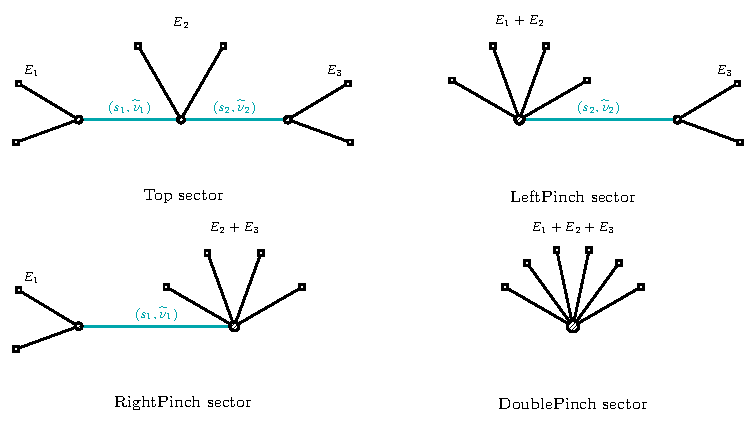
\includegraphics[width=0.88\textwidth]{figures/fig_tree_sectors.pdf}
  \caption{The four sectors of the three-vertex chain of figure~\ref{fig:tree-diagram},
  drawn in the same visual language.
  Contracting propagator~1 merges $L$ and $M$ (LeftPinch), contracting propagator~2 merges
  $M$ and $R$ (RightPinch), and both contractions merge all three vertices (DoublePinch).
  A merged component is drawn as a larger hatched circle carrying the external-leg fans of
  all vertices it contains, and the contracted propagator is
  absent; the surviving propagator keeps its mode-function two-state (massive chain) or shared
  (massless chain) slot and its teal label. All panels are drawn for equal contour signs. The
  massless chain of the regulator example (figure~\ref{fig:ep-tree}) carries the same
  four sectors.}
  \label{fig:tree-sectors}
\end{figure}
For other contour assignments, a propagator whose two
vertices carry opposite signs is theta-free and cannot be contracted, so only the allowed
pinched sectors appear.

We write $\sigma_{LM}$ and $\sigma_{MR}$ for the contour signs of the two internal propagators,
$+1$ for $G_{++}$ and $-1$ for $G_{--}$ as in \eqref{eq:massless-relations}. The lowering contact
term of the Top IBP at $v=L$ or $M$ is then the two-vertex relation \eqref{eq:R-two-vertex},
written in the indices of this graph,
\begin{equation}
  \cR^{(0)}_{v;\tilde{\bm r},\sigma_{LM}}
  =-\sigma_{LM}\,\delta_{a,1-b}\,(-1)^{a+1}\,\frac{4\ii}{\pi}\,s_1^{-2\nu_1-1}\,
   \text{I}_{\rm L}\bigl(-\bm e_{LM};(c,d)\bigr),
  \qquad \tilde{\bm r}=1+2c+d,
  \label{eq:tree-contact-term}
\end{equation}
where the child is taken at shift $-1$ on the merged component and $0$ on $\tau_R$, so that its
merged power is one below \eqref{eq:application-child-master}, and the bits $a,b$ of the contracted
propagator are removed from the parent string, leaving $\tilde{\bm r}$ as the packed label of $(c,d)$.
The four sectors then carry the hidden constants
\begin{equation}
  \begin{aligned}
  \cN_{\rm Top}&=1, & \cN_{\rm L}&=-\sigma_{LM}\,\frac{4\ii}{\pi}\,s_1^{-2\nu_1-1},\\
  \cN_{\rm R}&=-\sigma_{MR}\,\frac{4\ii}{\pi}\,s_2^{-2\nu_2-1}, &
  \cN_{\rm D}&=-\sigma_{LM}\sigma_{MR}\,\frac{16}{\pi^2}\,s_1^{-2\nu_1-1}s_2^{-2\nu_2-1},
  \end{aligned}
  \label{eq:tree-sector-normalizations}
\end{equation}
which is the product rule \eqref{eq:sector-normalization} with $\cN_s^{(0)}=1$, read in the
negative-prefactor convention, where $q_e^{2\nu_e-1}$ becomes $q_e^{-2\nu_e-1}$. The object the
package propagates in sector $s$ is $J_s(\bm n;\bm a)=\cN_s\,\text{I}_s(\bm n;\bm a)$ ---
concretely $J^{\boldsymbol\sigma}_{abcd}=\text{I}^{\boldsymbol\sigma}_{abcd}$,
$J^{\boldsymbol\sigma,{\rm L}}_{cd}=\cN_{\rm L}\text{I}^{\boldsymbol\sigma,{\rm L}}_{cd}$,
$J^{\boldsymbol\sigma,{\rm R}}_{ab}=\cN_{\rm R}\text{I}^{\boldsymbol\sigma,{\rm R}}_{ab}$ and
$J^{\boldsymbol\sigma,{\rm D}}=\cN_{\rm D}\text{I}^{\boldsymbol\sigma,{\rm D}}$ --- and for the
$(+++)$ assignment \eqref{eq:tree-sector-normalizations} is the value of the
\texttt{"normalization"} field of each master record.

At real kinematic points, we compute the four assignments
$(+++)$, $(++-)$, $(+-+)$ and $(-++)$.
After restoring the vertex factors and mode normalizations, each
$\text{I}^{\boldsymbol\sigma}_{0000}$ entry gives one contribution to the physical correlator.
Reversing all three contour signs gives the complex conjugate contribution, so the four computed
terms and their conjugates determine $\mathcal A_{\mathrm{phys}}$.
To match the phase convention above, the application code passes $-E_v$ as \texttt{externalLegEnergy}, uses \texttt{NuConvention -> "Negative"}, and supplies the corresponding pinch normalizations.

We set $p_1=p_2=p_3=0$ and express all energies and momenta in units of $E_2$.
With $q=s_1/E_2$, the scan follows
\begin{equation}
 \begin{aligned}
 (E_1,E_2,E_3,s_1,s_2)
 &=\left(\frac{100q}{99},1,\frac{10}{99},q,\frac{1}{10}\right),
 & (\nu_1,\nu_2)&=(\ii,2\ii),\\
 (\nu_{0L},\nu_{0M},\nu_{0R})
 &=\left(\frac32+\ii,3+3\ii,\frac32+2\ii\right).&&
 \end{aligned}
 \label{eq:tree-slice}
\end{equation}

As the numerical benchmark, which is independent of the DE construction, we use the multivariate
hypergeometric representation of this correlator derived
in \cite{Xianyu:2023ytd}.
It expresses the signal and background contributions as multiple series
containing Appell $F_2$ functions. Their sum gives the complete physical
correlator. These contributions are not the IBP sectors in
\eqref{eq:tree-hierarchy}.
For this benchmark, DE transport evolves the full master vector for each
contour assignment and then extracts the physical correlator from its
$\text{I}^{\boldsymbol\sigma}_{0000}$ entries. The hypergeometric calculation
evaluates the same physical correlator directly at each target point;
it does not separately evaluate all entries of the master vectors.
The reported comparison is therefore between physical correlators,
not an entry-by-entry comparison of all masters.
The truncation order is selected by comparing adjacent orders.
The reported hypergeometric time is the sum of the accepted
pointwise evaluation times.

The DE calculation uses 80 decimal digits and local Taylor series truncated at order 80.
An independent transport at order 96 provides an internal stability check.
We compare batches of $N=1$, $10$, $50$ and $100$ target points on the slice in \eqref{eq:tree-slice}.
For $N=1$, $10$ and $50$, transport starts at $q=0.1$ and ends at $q=10^{-4}$.
The single point is the end of the path, corresponding to $x=-\log_{10}q=4$.
The 10 points are selected at approximately equal index intervals from the 50 points of the
$N=50$ batch, including both ends.
The 100-point batch contains 80 points on this path and 20 additional points from $q=0.105$ to $0.2$.
The additional points share the boundary at $q=0.1$ but require transport in the opposite direction.

The hypergeometric times for these four batches are $22.78$, $344.62$, $1040.95$ and $4242.89\,\mathrm{s}$.
The corresponding median DE times are $26.71$, $48.82$, $48.86$ and $57.56\,\mathrm{s}$
(figure~\ref{fig:tree-timing}).
Each DE time covers data preparation, the Python invocation, boundary construction, DE generation
and the transport call, with the order-96 backend time subtracted.
All four DE batches were measured three times, with the execution order varied between rounds.
We report the median total time and show the full range of the three measurements.
The observed ratios of hypergeometric time to DE time are $7.06$, $21.31$ and $73.71$ for
$N=10$, $50$ and $100$, respectively.
For the single-point batch at the far end of the path, DE transport is slower than the
hypergeometric evaluation.

The average DE time per output point decreases from $26.71\,\mathrm{s}$ to $4.88$, $0.98$ and $0.58\,\mathrm{s}$ across these batches.
Boundary data and transport are shared, rather than recomputed independently for each target.
Points encountered along the path use saved node values or evaluations of an already constructed local series.
In these runs, each branch used 29 internal nodes for one output point and 33 nodes for
10 output points.
Thus, additional outputs did not require a proportional increase in transport work.

Within a convergence disk, a shorter step suppresses higher Taylor terms.
It can therefore permit a lower truncation order at a fixed accuracy.
This is a local property, not a guarantee of lower total cost, since shorter steps can require more segments.

\begin{figure}[H]
  \centering
  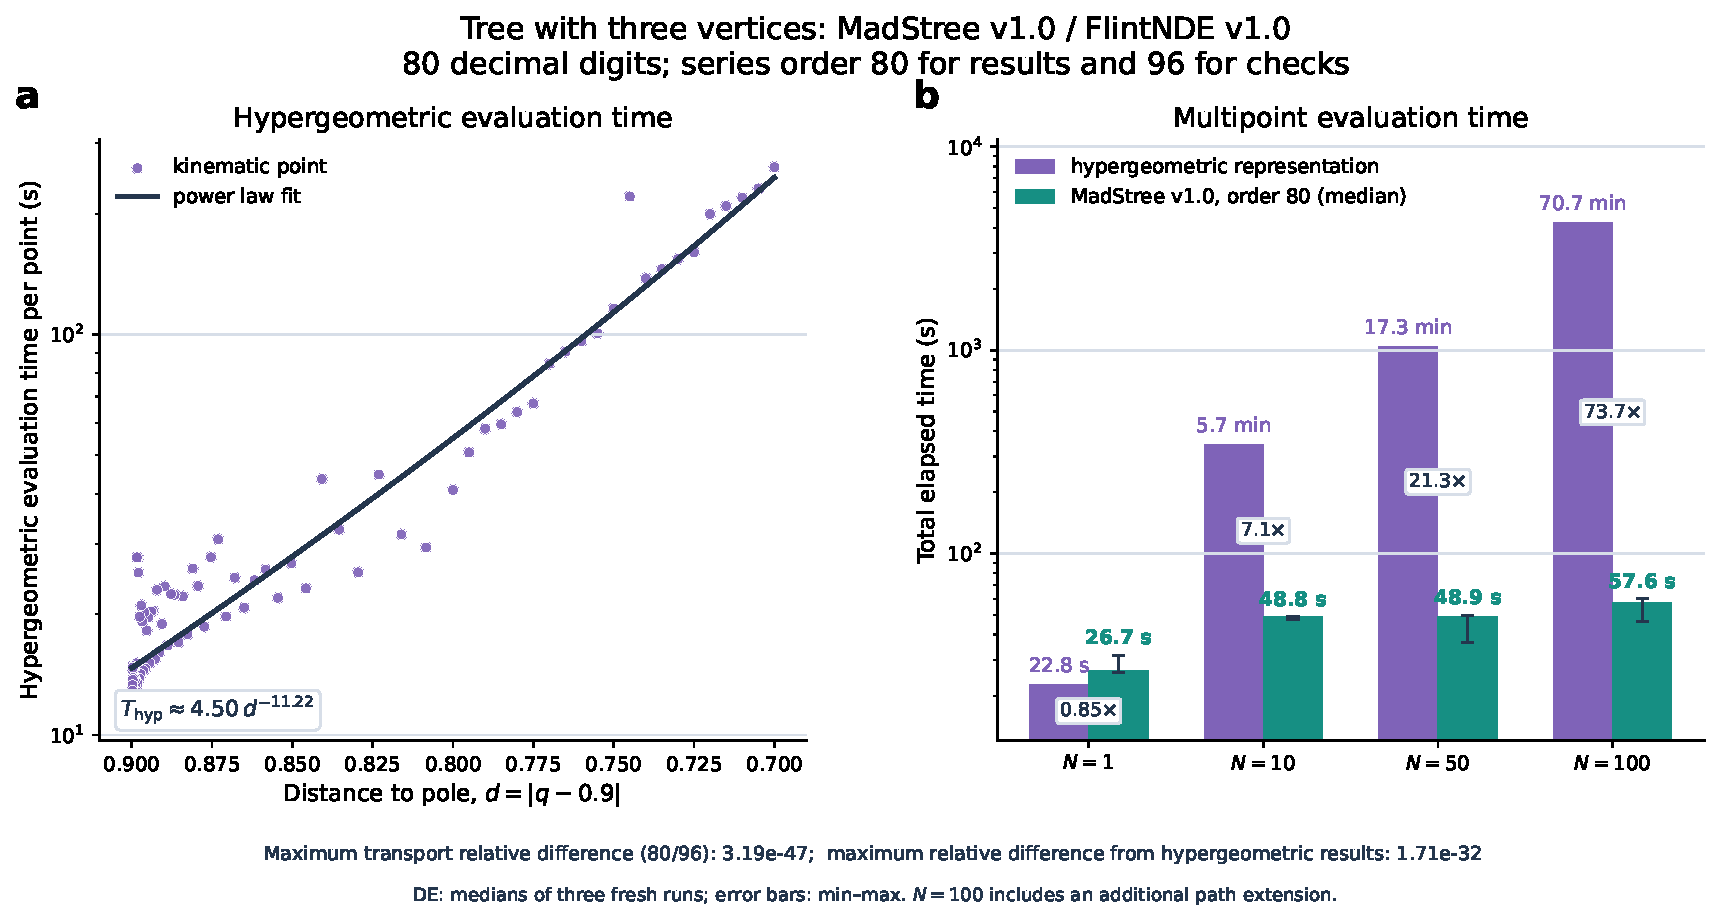
\includegraphics[width=0.99\textwidth]{figures/time.pdf}
  \caption{Tree benchmark with \texttt{MadStree} and \texttt{FlintNDE}.
  \textbf{a}, Hypergeometric evaluation time at individual kinematic points.
  \textbf{b}, Total evaluation times for $N=1$, $10$, $50$ and $100$ target points.}
  \label{fig:tree-timing}
\end{figure}

The 100 points in figure~\ref{fig:tree-timing}\textbf{a} comprise 80 points with
$q=10^{-x}$ and $x=1+3j/79$ ($j=0,\ldots,79$), uniformly spaced in $x$, and
20 points with $q=0.1+0.005j$ ($j=1,\ldots,20$), uniformly spaced in $q$.
Each hypergeometric time is measured at the accepted truncation order.
In panel \textbf{b}, the DE bars show medians of three runs, with error bars spanning the minimum and maximum.
The first three batches share the same start and end; the 100-point batch includes the additional
path extension.
Hypergeometric data are newly computed for $N=1$ and $10$ and retained for $N=50$ and $100$.
The ratio labels give the hypergeometric time divided by the DE time.
The figure footer reports the maximum relative differences between the two transport orders, and
between the DE and hypergeometric results, across all four batches.

Across the scan of 100 points, the maximum relative difference from the
hypergeometric result is $1.712\times10^{-32}$.
The comparison of transport orders 80 and 96 gives a maximum relative difference
of $1.308\times10^{-50}$.
At $x=4$, the physical correlator is
\begin{equation}
  \mathcal A_{\mathrm{phys}}(4)=9.87033514798954\times10^{-9},
\end{equation}
with a relative difference of $4.21\times10^{-36}$ from the hypergeometric result.

For the same kinematic configuration, the direct Appell $F_2$ representation
requires $q<0.89$.
The point $q=0.8905$ lies outside this domain, whereas the nearest positive
pole of the DE connection is at $q=0.9$.
To reach $q=1$, we continue the chosen analytic branch along
\begin{equation}
  0.1\to0.86\to0.86+0.04\ii\to0.93+0.04\ii\to0.93\to1.
  \label{eq:tree-contour}
\end{equation}
This contour avoids the pole through the upper half of the complex plane.
The continuation records 81 points.
The calculation at order 80 takes $35.08$~s, or $45.76$~s when the reference calculation at order 96 is included.
The maximum relative difference between orders 80 and 96 is $1.802\times10^{-44}$.
The DE method thus evaluates the selected analytic branch beyond the
domain of the direct series representation.

\begin{figure}[H]
  \centering
  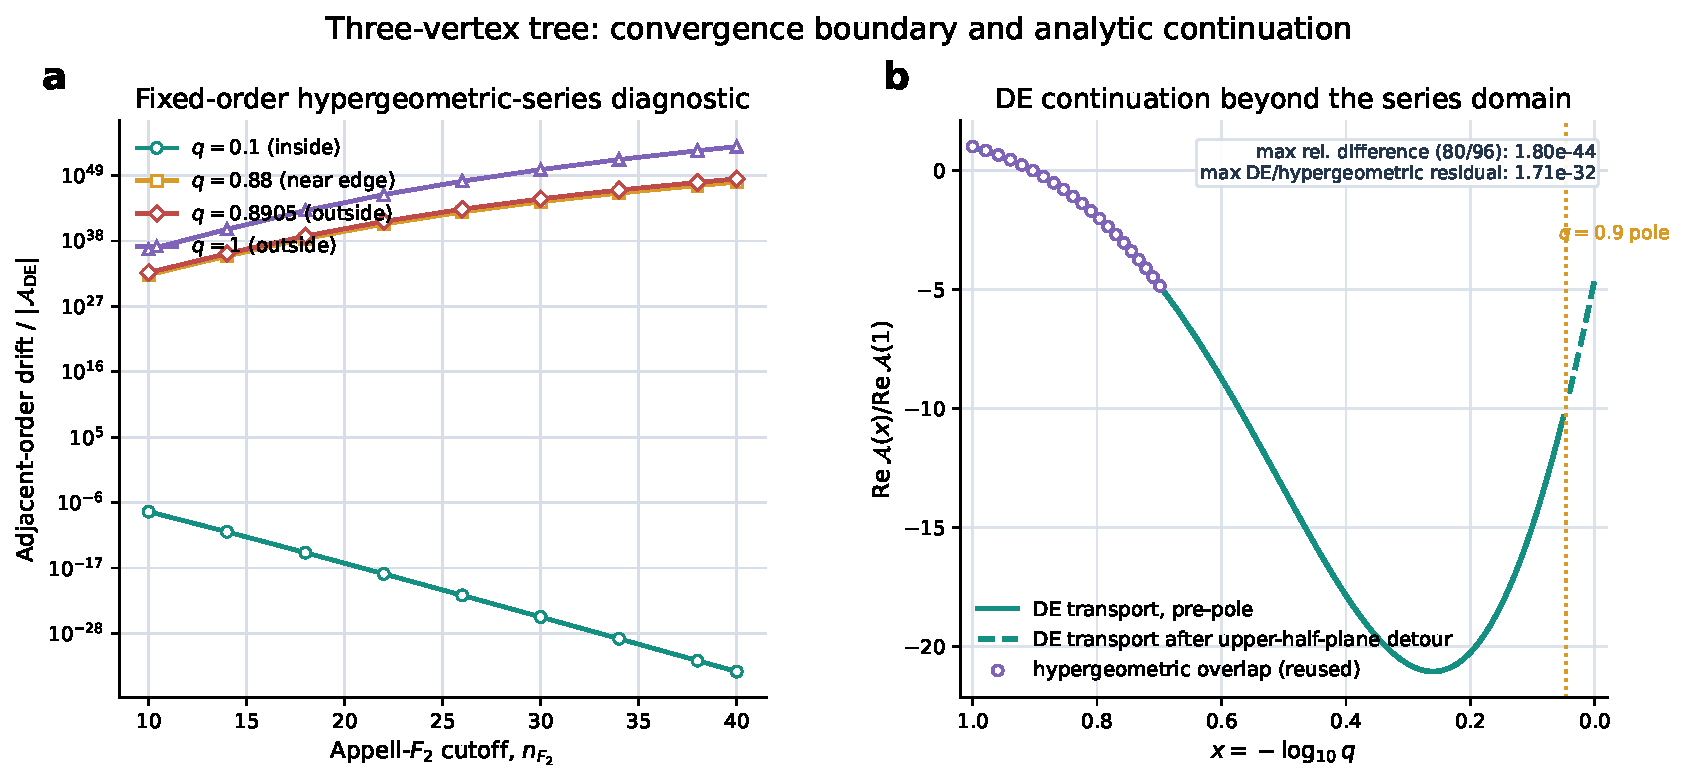
\includegraphics[width=0.99\textwidth]{figures/domain1.pdf}
  \caption{Analytic continuation with \texttt{MadStree}.
  \textbf{a}, Dependence of the hypergeometric partial sums on the truncation
  order near the direct convergence boundary.
  \textbf{b}, DE continuation at order 80 along the contour
  in \eqref{eq:tree-contour}.}
  \label{fig:tree-continuation}
\end{figure}

\paragraph{Bubble time kernel at fixed loop momentum}

The second example has two time vertices joined by two massive propagators
(figure~\ref{fig:bubble-diagram}).
We evaluate the integrals over the two vertex times while holding the internal
momenta fixed. We do not integrate over the spatial loop momentum.
\begin{figure}[H]
  \centering
  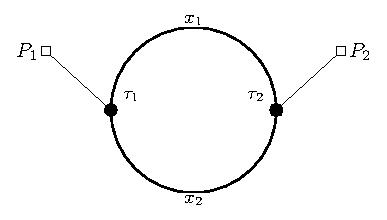
\includegraphics[width=0.55\textwidth]{figures/fig_bubble_diagram.pdf}
  \caption{Bubble time kernel, drawn with the in-in Feynman rules of
  Sec.~\ref{sec:conventions} for the assignment $pp$: both vertices are hatched circles
  on the \texttt{"+"} branch and carry the times $\tau_1,\tau_2$ and powers $p_1,p_2$ in the labels
  $V_1(\tau_1,p_1)$, $V_2(\tau_2,p_2)$ below the loop; each vertex carries a schematic fan
  of two external legs ending in open squares and labeled by the energy sums
  $P_1,P_2$. The two massive propagators join the same pair of vertices and are drawn as
  the two halves of one circular loop --- propagator~1 with momentum magnitude $x_1$ and
  mass label $\widetilde\nu_{B1}$ on the upper half, propagator~2 with $x_2$ and
  $\widetilde\nu_{B2}$ on the lower half.}
  \label{fig:bubble-diagram}
\end{figure}

From figure~\ref{fig:bubble-diagram}, the function family of this example has two time
integrals, one per vertex, and two propagator kernels, both joining the same pair of vertices; as
in the first example each kernel carries the mode-function states of its two endpoints.
Let $\tau_1,\tau_2$ be the vertex times, $P_1,P_2$ the external energy sums,
and $x_1,x_2$ the internal momentum magnitudes.
The Hankel orders of the two internal propagators are $\nu_{B1},\nu_{B2}$.
With the products $\mathcal G_{\sigma\sigma',\nu;ab}$ of
\eqref{eq:application-line-products} and \eqref{eq:sk-propagators}, the Top masters are
\begin{equation}
 \begin{aligned}
 \text{I}^{\sigma_1\sigma_2}_{abcd}
 ={}&\int_{-\infty}^{0}d\tau_1\,d\tau_2\,
 (-\tau_1)^{p_1}(-\tau_2)^{p_2}
 e^{\ii(\sigma_1P_1\tau_1+\sigma_2P_2\tau_2)}\\
 &\times\mathcal G_{\sigma_1\sigma_2,\nu_{B1};ab}(x_1;\tau_1,\tau_2)
 \mathcal G_{\sigma_1\sigma_2,\nu_{B2};cd}(x_2;\tau_1,\tau_2).
 \end{aligned}
 \label{eq:bubble-indexed-masters}
\end{equation}
Here $a,b,c,d\in\{0,1\}$. As in the first example, $a,b$ label the mode-function states of
propagator~1 at vertices~1 and~2, and $c,d$ those of propagator~2 in the same vertex order.
Here $p_1,p_2$ are the effective time powers after absorbing the mode
prefactors, unlike the bare powers used in \eqref{eq:tree-time-power-map}.
The contour signs are $\sigma_1,\sigma_2=\pm1$.
We denote positive and negative signs by $p$ and $m$, respectively;
these labels are unrelated to the time powers $p_1,p_2$.
The four contour assignments are $pp$, $pm$, $mp$ and $mm$.
An assignment with equal contour signs has 22 masters after the
exact mode-function state projection; an assignment with opposite contour signs has only the
Top sector, with 16 masters.
For each assignment, the projection onto the Top sector is
\begin{equation}
 \begin{aligned}
 \bm{\text I}^{\sigma_1\sigma_2}_{\rm Top}
 =\bigl(&\text{I}^{\sigma_1\sigma_2}_{0000},
        \text{I}^{\sigma_1\sigma_2}_{0001},
        \text{I}^{\sigma_1\sigma_2}_{0010},
        \text{I}^{\sigma_1\sigma_2}_{0011},
        \text{I}^{\sigma_1\sigma_2}_{0100},
        \text{I}^{\sigma_1\sigma_2}_{0101},
        \text{I}^{\sigma_1\sigma_2}_{0110},
        \text{I}^{\sigma_1\sigma_2}_{0111},\\
       &\text{I}^{\sigma_1\sigma_2}_{1000},
        \text{I}^{\sigma_1\sigma_2}_{1001},
        \text{I}^{\sigma_1\sigma_2}_{1010},
        \text{I}^{\sigma_1\sigma_2}_{1011},
        \text{I}^{\sigma_1\sigma_2}_{1100},
        \text{I}^{\sigma_1\sigma_2}_{1101},
        \text{I}^{\sigma_1\sigma_2}_{1110},
        \text{I}^{\sigma_1\sigma_2}_{1111}\bigr)^{\mathsf T},
 \end{aligned}
 \label{eq:bubble-top-vector}
\end{equation}
one for each of the sixteen values of $(a,b,c,d)\in\{0,1\}^4$.
The two pinched sectors of an equal-sign assignment arise from contracting one of the two
propagators. Both vertices then merge into a single component carrying one time $\tau$, and the
surviving propagator joins this component to itself. At coincident endpoints the theta pair of
the full propagator collapses and its factor becomes the mean of the two chamber products, the
spectator factor $\mathsf m_e$ of \eqref{eq:bundle-odd-subsets},
\begin{equation}
 T_{cd}(x;\tau)
 =\tfrac12\Big[h^{(1)}(\nu,c;-x\tau)\,h^{(2)}(\nu,d;-x\tau)
 +h^{(2)}(\nu,c;-x\tau)\,h^{(1)}(\nu,d;-x\tau)\Big],
 \label{eq:bubble-tadpole-kernel}
\end{equation}
which is symmetric under $(c,d)\leftrightarrow(d,c)$, so the coincidence quotient identifies
$(1,0)$ with $(0,1)$ and keeps the three combinations $(0,0),(0,1),(1,1)$ of the two endpoint
states --- this is the exact mode-function state
projection quoted above. The pinched masters are therefore, with propagator~1 contracted,
\begin{equation}
 \text{I}^{\sigma_1\sigma_2,{\rm P1}}_{cd}
 =\int_{-\infty}^{0}\dd\tau\,
 (-\tau)^{p_1+p_2+2\nu_{B1}}
 e^{\ii(\sigma_1P_1+\sigma_2P_2)\tau}\,
 T_{cd}(x_2;\tau),
 \qquad (c,d)\in\{(0,0),(0,1),(1,1)\},
 \label{eq:bubble-pinch1-masters}
\end{equation}
where the merged power follows from \eqref{eq:base-power} with the raw contact power
$\varrho_1=2\nu_{B1}-1$ and one vertex merge, and, with propagator~2 contracted,
\begin{equation}
 \text{I}^{\sigma_1\sigma_2,{\rm P2}}_{ab}
 =\int_{-\infty}^{0}\dd\tau\,
 (-\tau)^{p_1+p_2+2\nu_{B2}}
 e^{\ii(\sigma_1P_1+\sigma_2P_2)\tau}\,
 T_{ab}(x_1;\tau),
 \qquad (a,b)\in\{(0,0),(0,1),(1,1)\}.
 \label{eq:bubble-pinch2-masters}
\end{equation}
The equal-sign hierarchy is
$\mathrm{Top}(16)\oplus\mathrm{Pinch}_1(3)\oplus\mathrm{Pinch}_2(3)$ with $\dim=22$
(figure~\ref{fig:bubble-sectors}).
\begin{figure}[H]
  \centering
  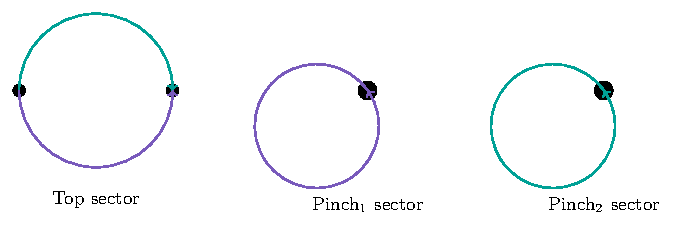
\includegraphics[width=0.85\textwidth]{figures/fig_bubble_sectors.pdf}
  \caption{The three sectors of the bubble time kernel of
  figure~\ref{fig:bubble-diagram}, drawn for the equal-sign assignments ($pp$ and $mm$)
  and with the same colors as in figure~\ref{fig:bubble-diagram}: the Top sector keeps
  both propagators of the circular loop;
  Pinch$_1$ contracts propagator~1 (upper half, $x_1$) and leaves propagator~2 as a
  circular tadpole on the single merged vertex, drawn as a larger hatched circle carrying
  both external-leg fans; Pinch$_2$ contracts
  propagator~2 and leaves propagator~1. The opposite-sign assignments $pm$ and $mp$ have
  only the Top sector.}
  \label{fig:bubble-sectors}
\end{figure}
The vertex factors $(\ii\sigma_1)(\ii\sigma_2)$ give
\begin{equation}
  \bm K_{\mathrm{SK}}=-\bm{\text I}^{pp}_{\rm Top}+\bm{\text I}^{pm}_{\rm Top}
  +\bm{\text I}^{mp}_{\rm Top}-\bm{\text I}^{mm}_{\rm Top}.
  \label{eq:bubble-sk}
\end{equation}
Only the equal-sign assignments reach a pinched sector, and there both propagators are of one
branch, so they share the contour sign $\sigma_e=\sigma_1=\sigma_2$ of
\eqref{eq:sector-normalization}. The hidden constants of the three sectors are
\begin{equation}
  \cN_{\rm Top}=1,\qquad
  \cN_{\rm P1}=-\sigma_e\,\frac{4\ii}{\pi}\,x_1^{\,2\nu_{B1}-1},\qquad
  \cN_{\rm P2}=-\sigma_e\,\frac{4\ii}{\pi}\,x_2^{\,2\nu_{B2}-1},
  \label{eq:bubble-sector-normalizations}
\end{equation}
with $\cN_s^{(0)}=1$; the propagated objects are
$J^{\sigma_1\sigma_2}_{abcd}=\text{I}^{\sigma_1\sigma_2}_{abcd}$,
$J^{\sigma_1\sigma_2,{\rm P1}}_{cd}=\cN_{\rm P1}\text{I}^{\sigma_1\sigma_2,{\rm P1}}_{cd}$ and
$J^{\sigma_1\sigma_2,{\rm P2}}_{ab}=\cN_{\rm P2}\text{I}^{\sigma_1\sigma_2,{\rm P2}}_{ab}$.
This example runs in the package default convention, so the power is the
$2\nu_e-1$ of \eqref{eq:sector-normalization} rather than the $-2\nu_e-1$ of the tree example.
We use $k_s=x_1$ as the momentum unit and vary the dimensionless energy
$\rho=P_1/k_s=P_2/k_s$. The parameter values in
\eqref{eq:bubble-indexed-masters} are
\begin{equation}
 \begin{aligned}
 (k_s,x_1,x_2)&=(1,1,\sqrt2),\qquad P_1=P_2=\rho,\\
 (\nu_{B1},\nu_{B2})&=(\ii/4,\ii/4),\qquad
 p_1=p_2=1+\ii/2.
 \end{aligned}
 \label{eq:bubble-parameters}
\end{equation}
The normalized $0000$ entry of $\bm K_{\mathrm{SK}}$, written $\widehat K_{\mathrm{SK}}(\rho)$, is
\begin{equation}
  \widehat K_{\mathrm{SK}}(\rho)
  =\frac{[\bm K_{\mathrm{SK}}(\rho)]_{0000}}
  {[\bm K_{\mathrm{SK}}(10)]_{0000}}.
  \label{eq:bubble-normalized}
\end{equation}
The four zeros select the four undifferentiated mode-function states of the two massive propagators.

The scan contains 201 points over $2.8\leq\rho\leq10$.
Calculations use decimal arithmetic with 80 digits. The transport orders are
80 and 96, and the boundary series orders are 17 and 15.
The calculation time excluding reference transport at order 96 is $678.20$~s.
It includes all four contour assignments, DE construction and both
boundary calculations.
The reference transport takes $5.24$~s, and the total recorded time is
$683.43$~s.
The average cost for the scan, including setup, is $3.37$~s per point.
This average is not the cost of a calculation at a single point.

The maximum relative difference between boundary orders 17 and 15 is
$4.740\times10^{-24}$.
The maximum relative difference between transport orders 80 and 96 is
$1.025\times10^{-50}$.
These tests assess boundary and transport stability separately; the
comparison of transport orders alone is not a bound on the total error.

\begin{figure}[H]
  \centering
  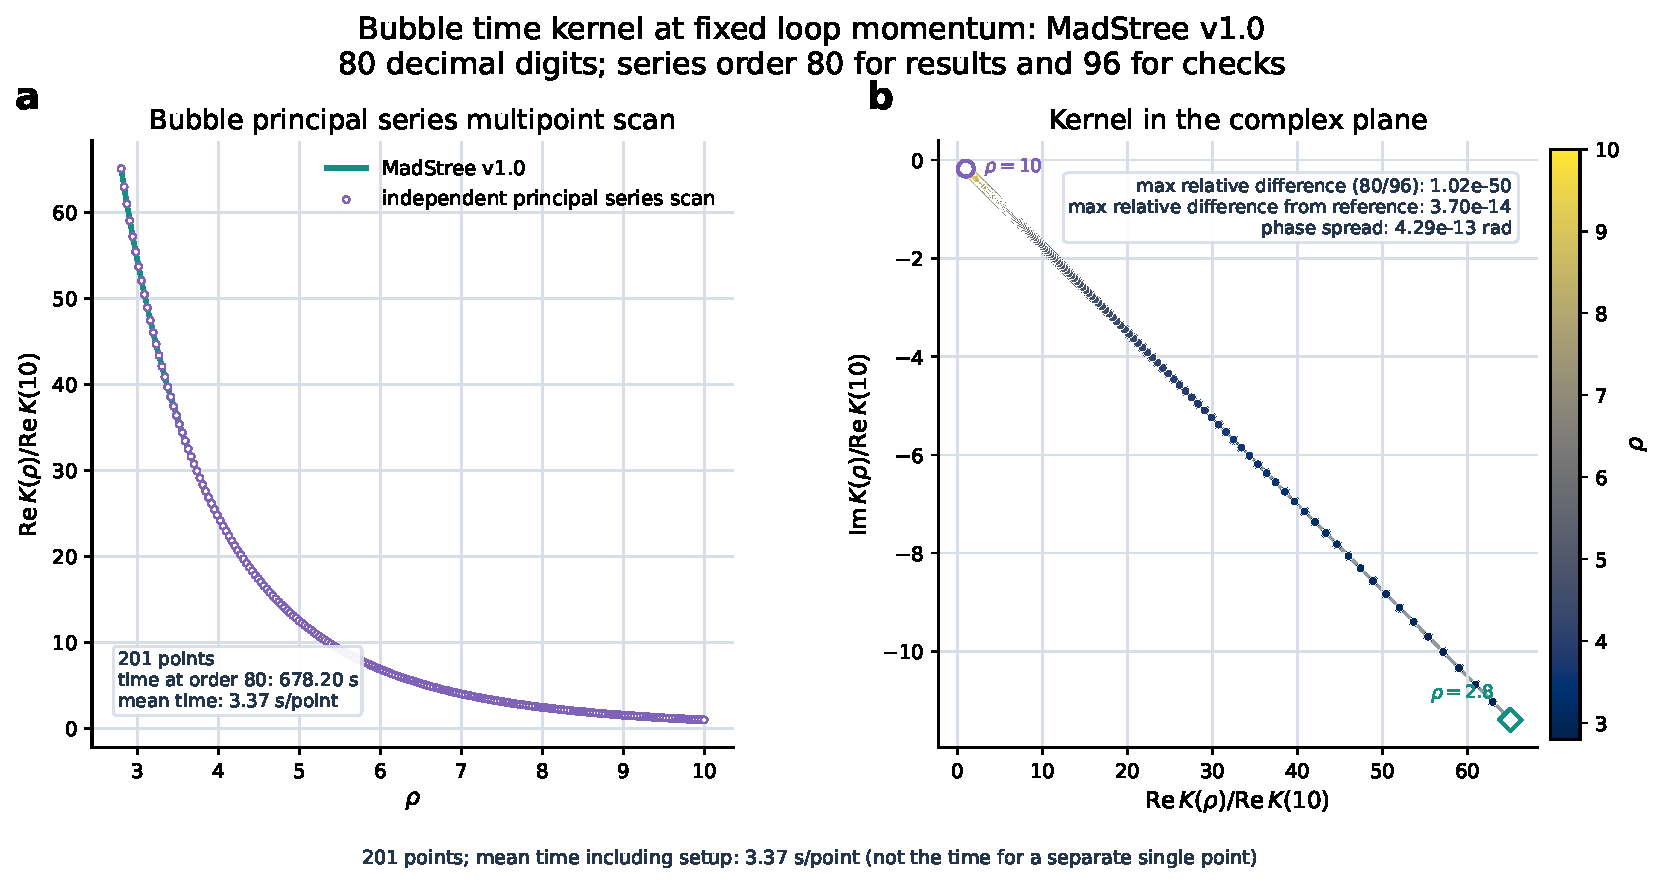
\includegraphics[width=0.99\textwidth]{figures/bubble2.pdf}
  \caption{Bubble time kernel evaluated with \texttt{MadStree}.
  \textbf{a}, The normalized kernel and the independent reference.
  \textbf{b}, The kernel in the complex plane, with color indicating $\rho$.}
  \label{fig:bubble-scan}
\end{figure}

Both panels of figure~\ref{fig:bubble-scan} use the same 201 points. Panel \textbf{a} compares the
normalized kernel \eqref{eq:bubble-normalized} with the same quantity computed by a separate program
written for this bubble graph alone, which does not use \texttt{MadStree}; the maximum relative
difference over the scan is $3.70\times10^{-14}$. The nearly radial
distribution in panel \textbf{b} indicates an approximately constant phase.

\paragraph{Massless three-vertex tree in the regulator mode}

The third example returns to the chain topology of the first example with both exchanges
massless, and lowers the time power of vertex~1 by two units before shifting all vertex time
powers by the common analytic regulator (figure~\ref{fig:ep-tree}): $a_1=-1+\varepsilon$,
$a_2=a_3=1+\varepsilon$. At $\varepsilon=0$ the time integrals of this graph genuinely
diverge, which is the situation the regulator mode of Sec.~\ref{sec:regulator} is designed for:
the computation is defined at the regularized powers, and requesting the return level
$\varepsilon^0$ delivers both the $\varepsilon^{-1}$ pole coefficient and the finite part. The
momenta are fixed by
\texttt{ParameterRules} and the target point is $\{k_1,k_2,k_3\}=\{9\ii,3\ii,5\ii\}$.
\begin{figure}[H]
  \centering
  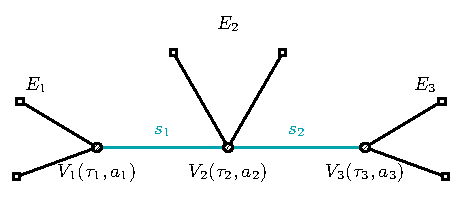
\includegraphics[width=0.72\textwidth]{figures/fig_ep_tree.pdf}
  \caption{Massless three-vertex chain in the regulator mode, drawn as in
  figure~\ref{fig:tree-diagram} with the massless counterparts of its parameters: the same
  external-leg fans with summed energies $E_v=\sum_j k_{v,j}$ and propagator momentum
  magnitudes $s_1,s_2$, with no mass labels since the massless propagators carry the
  fixed order $\nu=1/2$. The vertex labels $V_v(\tau_v,a_v)$ below the vertices carry the
  regularized time powers $a_1=-1+\varepsilon$ and $a_2=a_3=1+\varepsilon$, i.e. the time
  factors $(-\tau_1)^{-1+\varepsilon}$, $(-\tau_2)^{1+\varepsilon}$ and
  $(-\tau_3)^{1+\varepsilon}$. The fans are schematic --- in the input of Example~06 each
  vertex carries a single external leg, $E_v=k_v$, $s_1=q_{12}$ and $s_2=q_{23}$ --- and
  the input fixes all three vertices to the \texttt{"+"} branch, so this example
  evaluates the all-plus assignment $(+++)$ only.}
  \label{fig:ep-tree}
\end{figure}
The input is
\begin{verbatim}
treeSpec = <|
  "vertices" -> {
    <|"id" -> 1, "externalLegEnergy" -> k1,
      "timePower" -> a1, "vertexType" -> "+"|>,
    <|"id" -> 2, "externalLegEnergy" -> k2,
      "timePower" -> a2, "vertexType" -> "+"|>,
    <|"id" -> 3, "externalLegEnergy" -> k3,
      "timePower" -> a3, "vertexType" -> "+"|>},
  "lines" -> {
    <|"type" -> "massless", "endpoints" -> {1, 2},
      "momentum" -> q12, "nu" -> 1/2|>,
    <|"type" -> "massless", "endpoints" -> {2, 3},
      "momentum" -> q23, "nu" -> 1/2|>}|>;
context = MSInitTree[treeSpec];
epSeries = MSReconstructEpSeries[context, ep,
  {{k1, k2, k3}, {9 I, 3 I, 5 I}},
  ParameterRules -> {q12 -> 1, q23 -> 2,
    a1 -> -1 + ep, a2 -> 1 + ep, a3 -> 1 + ep},
  MaximumEpPower -> 0, EpGoalDigits -> 12,
  EpSampleAngleRange -> {-Pi/3, Pi/3},
  RankOrder -> {1, 2, 3}]
\end{verbatim}
The example additionally sets \texttt{BoundaryScale -> 4}, \texttt{BoundarySeriesOrder -> 24}
and the default pool of \texttt{ParallelTaskCount -> 12} workers.

From figure~\ref{fig:ep-tree}, the family has three time integrals and two propagator kernels;
because both propagators are massless full propagators of the fixed order $\nu=1/2$, each
contributes one shared mode-function two-state slot (Sec.~\ref{sec:massless}) rather than two
independent endpoint mode-function states.
We keep the parameter conventions of the first example: $E_v$ denotes the external energy sum of
vertex $v$ --- here the single input energy $k_v$ --- and $s_1,s_2$ the internal momentum
magnitudes, in the input $q_{12},q_{23}$. At $\nu=1/2$ both compressed mode-function states are
pure exponentials, \eqref{eq:h-branch-eigenvalues}, so the input time powers $a_v$ are the
effective integrand powers and no map like \eqref{eq:tree-time-power-map} is needed. With the
contour sign $\sigma_e=\pm1$ of a full propagator, as in \eqref{eq:massless-relations}, the
shared mode-function two-state slot $b_e\in\{0,1\}$ of Sec.~\ref{sec:massless} enters through the compressed
kernel
\begin{equation}
 \begin{aligned}
 \mathcal G^{\rm m}_{\sigma_e,b}(s_e;\tau_u,\tau_v)
 ={}&(\ii\sigma_e)^{b}\,\theta_{uv}\,
    h^{(1)}\!\left(\tfrac12,0;-s_e\tau_u\right)
    h^{(2)}\!\left(\tfrac12,0;-s_e\tau_v\right)\\
 &+(-\ii\sigma_e)^{b}\,\theta_{vu}\,
    h^{(2)}\!\left(\tfrac12,0;-s_e\tau_u\right)
    h^{(1)}\!\left(\tfrac12,0;-s_e\tau_v\right),
 \end{aligned}
 \label{eq:ep-massless-kernel}
\end{equation}
whose two entries are the sum and difference of the two chambers, the slot vector
$\bm g_e=(\text{I}_{00},\text{I}_{10})^{\mathsf T}$ of \eqref{eq:SP-massless}. With one such
shared slot per propagator, the Top sector has the four masters
\begin{equation}
 \begin{aligned}
 \text{I}^{\boldsymbol\sigma}_{b_1b_2}
 ={}&\int_{-\infty}^{0}\dd\tau_1\,\dd\tau_2\,\dd\tau_3\,
 (-\tau_1)^{a_1}(-\tau_2)^{a_2}(-\tau_3)^{a_3}
 e^{\ii(\sigma_1E_1\tau_1+\sigma_2E_2\tau_2+\sigma_3E_3\tau_3)}\\
 &\times\mathcal G^{\rm m}_{\sigma_1\sigma_2,b_1}(s_1;\tau_1,\tau_2)\,
 \mathcal G^{\rm m}_{\sigma_2\sigma_3,b_2}(s_2;\tau_2,\tau_3),
 \qquad b_1,b_2\in\{0,1\},
 \end{aligned}
 \label{eq:ep-top-masters}
\end{equation}
with the bits taken in propagator order, and the Top vector is
$(\text{I}^{\boldsymbol\sigma}_{00},\text{I}^{\boldsymbol\sigma}_{01},
\text{I}^{\boldsymbol\sigma}_{10},\text{I}^{\boldsymbol\sigma}_{11})^{\mathsf T}$.
A contracted massless propagator has the raw contact power $\varrho=0$ of \eqref{eq:base-power},
and its pure exponentials multiply into the merged exponential. The four sectors, shown in
figure~\ref{fig:tree-sectors}, are
\begin{equation}
 \begin{aligned}
 \text{I}^{\boldsymbol\sigma,{\rm L}}_{b}
 ={}&\int_{-\infty}^{0}\!\!\dd\tau_{12}\!\int_{-\infty}^{0}\!\!\dd\tau_3\,
 (-\tau_{12})^{a_1+a_2+1}(-\tau_3)^{a_3}
 e^{\ii(\sigma_1E_1+\sigma_2E_2)\tau_{12}+\ii\sigma_3E_3\tau_3}\\
 &\times\mathcal G^{\rm m}_{\sigma_2\sigma_3,b}(s_2;\tau_{12},\tau_3),
 \qquad b\in\{0,1\},
 \end{aligned}
 \label{eq:ep-left-masters}
\end{equation}
where propagator~1 is contracted and $\tau_{12}$ is the time of the merged component,
\begin{equation}
 \begin{aligned}
 \text{I}^{\boldsymbol\sigma,{\rm R}}_{b}
 ={}&\int_{-\infty}^{0}\!\!\dd\tau_1\!\int_{-\infty}^{0}\!\!\dd\tau_{23}\,
 (-\tau_1)^{a_1}(-\tau_{23})^{a_2+a_3+1}
 e^{\ii\sigma_1E_1\tau_1+\ii(\sigma_2E_2+\sigma_3E_3)\tau_{23}}\\
 &\times\mathcal G^{\rm m}_{\sigma_1\sigma_2,b}(s_1;\tau_1,\tau_{23}),
 \qquad b\in\{0,1\},
 \end{aligned}
 \label{eq:ep-right-masters}
\end{equation}
with propagator~2 contracted, and the single one-time master of the DoublePinch sector,
\begin{equation}
 \text{I}^{\boldsymbol\sigma,{\rm D}}
 =\int_{-\infty}^{0}\dd\tau\,
 (-\tau)^{a_1+a_2+a_3+2}
 e^{\ii(\sigma_1E_1+\sigma_2E_2+\sigma_3E_3)\tau}.
 \label{eq:ep-double-master}
\end{equation}
The hierarchy is therefore
$\mathrm{Top}(4)\oplus\mathrm{LeftPinch}(2)\oplus\mathrm{RightPinch}(2)\oplus
\mathrm{DoublePinch}(1)$ with $\dim=9$, the nine-dimensional DE recorded in
Sec.~\ref{sec:examples}; the massive chain of \eqref{eq:tree-hierarchy} carries four mode-function state slots
and $25$ masters. No contracted propagator contributes a pinch factor in
\eqref{eq:sector-normalization}, so every sector normalization is $1$, $J_s=\text{I}_s$ here,
and the propagated vector is the master vector $\bm{\text I}$ itself, in the convention of
\eqref{eq:tree-indexed-masters} without vertex contour factors.

The certificate of Sec.~\ref{sec:regulator} runs before any numerical solve and returns
$n_{\min}=-1$: the d log-form DE is regular at $\varepsilon=0$, but the vertex-1 unit
$u_1=a_1+1=\varepsilon$ is isolated as a standalone factor in part of the factorized boundary
weights, and every such branch carries a single $\Gamma(\varepsilon)$ simple pole, so the
combined physical boundary starts at $\varepsilon^{-1}$ with component valuations $-1$ or
$0$ only. Three Frobenius recurrence operators do drop rank at $\varepsilon=0$, with rank
changes $9\to5$, $9\to8$ and $9\to8$ at the exponents $6(1+\varepsilon)$ (twice) and
$8+7\varepsilon$; per
Sec.~\ref{sec:regulator} these are retained as resonance diagnostics and produce no additional
pole, since the combined physical boundary decides the support. With $m=0$, $n_{\min}=-1$ and
$g=12$, \eqref{eq:regulator-fit-count} and \eqref{eq:regulator-scale-precision} give
$P=1$, $\Delta=1$, $N_{\rm fit}=4$, $\alpha_\varepsilon=25/4$, $\varepsilon_0=10^{-25/4}$,
$p_0=32$, a working
precision of $200$ digits and a primary transport order of $128$ with $50$ reference orders.
The four production points are exact Gaussian rationals of moduli
$\varepsilon_0(1+j/100)$, $j=1,\ldots,4$, cycling through the rays $-\pi/6$, $0$ and $+\pi/6$ of the
open window $(-\pi/3,\pi/3)$; the two validation points sit at half the first two moduli, on the
rays $-\pi/6$ and $0$, and never enter the fit. All six solves are dispatched to one bounded pool
($12$ requested, $6$ effective); the whole reconstruction, including the certificate, both
validation solves and the fit, takes $170$~s of wall time.

The returned Laurent data are the $\varepsilon^{-1}$ pole coefficient and the
$\varepsilon^0$ coefficient, both $9$-entry master vectors. Entries below $10^{-20}$ in
absolute value are numerical noise at the achieved accuracy and are reported as zero. For scale,
the relative validation residual is of order $10^{-25}$, while the physical entries are of order
$10^{-3}$ or larger. With this convention three entries of the pole coefficient vanish,
among them the DoublePinch entry, because the fully merged boundary branch carries no
isolated $\Gamma(\varepsilon)$ factor. Two representative entries are
\begin{equation}
  \begin{aligned}
  [c_{-1}]_{\mathrm{Top},00}&=\bigl(9.49200055589-25.86650516658\,\ii\bigr)\times10^{-4},\\
  [c_0]_{\mathrm{D}}&=7.18382203278\times10^{-5},
  \end{aligned}
  \label{eq:ep-finite-entries}
\end{equation}
The first is the Top-sector entry with both shared slots in their symmetric state, $b_1=b_2=0$,
and the second is the DoublePinch master, a single one-time integral. At the two independent
validation points the fitted series is summed over all four internal powers
$\varepsilon^{-1},\ldots,\varepsilon^{2}$, which include the two buffer powers above the requested
maximum $m=0$. Compared with the directly transported values it reaches a maximum relative residual
of $7.43\times10^{-25}$, thirteen orders below the requested tolerance $10^{-12}$. That residual
certifies the fit against this tolerance, not a number of correct digits: the coefficients are computed
at a working precision of $200$ digits and returned with about $199$ significant digits. This example
runs the whole regulator procedure of Sec.~\ref{sec:regulator} on a genuinely divergent
configuration: the sampling grid and the precisions follow from the certified lowest power, and the
pole coefficient and the finite part of the $\varepsilon\to0$ Laurent expansion are delivered
together with an explicit validation residual.

The tree example illustrates two uses of DE transport: efficient multipoint
evaluation and continuation beyond the convergence domain of a direct series.
The bubble example applies the same framework for time integrals to a graph
containing a loop at fixed internal momenta.
The regulator example certifies the Laurent support symbolically on a divergent
massless chain and delivers the $\varepsilon\to0$ pole coefficient and finite part from six
numerical solves.




\section{Verification against independent references}
\label{sec:verification}

The package was checked against independent references in the following verification tasks.

\begin{itemize}
  \item \textbf{Single-vertex families and the massive two-vertex correlator.} The exact
        differential equations, the boundary coefficients and the numerically transported results
        are compared with the known results of \cite{Chen:2024glu}, which are computed by an
        independent multivariate hypergeometric construction.
  \item \textbf{The massive three-vertex tree graph.} The package results are checked against two
        independent sources at once: the output of an agent program that received only the
        previously hand-written two-vertex code and generalized it to three vertices by its own
        method, and the published eight-branch result of \cite{Xianyu:2023ytd}. The agent output was
        itself first checked against that published result before being used as a reference, so the
        package is validated both by independently generated code and by the published numbers.
  \item \textbf{IBP relations and differential equations.} These are compared with the output of the
        \texttt{dSIBP} package \cite{dSIBP:inPreparation}, which is released in the same repository
        as this one, \url{https://github.com/J7C/dSIBP-Packages}. \texttt{dSIBP} samples naive IBP
        seeds and solves the resulting linear reduction system, whereas the present package applies
        the general formulas derived in Sec.~\ref{sec:method} directly and never re-solves an IBP
        system; the agreement therefore tests the closed formulas themselves.
\end{itemize}

\section{Summary and outlook}
\label{sec:summary}

\texttt{MadStree} implements the general IBP and d log-form construction of
\cite{Chen:2023iix,Chen:2024glu} as a single computation that starts from the diagram the user
supplies and ends at kinematic points, with no intermediate formula written by hand. Three local
blocks --- the theta-free vertex exponential, the massive mode-function two-state block, and the massless block
whose four mode-function states compress into one shared mode-function two-state factor --- feed one registry, and that registry
alone gives the iterative reduction, the uniform d log-form differential equation, and the contact
terms that merge vertices under a common theta function. The boundary data come from the same
objects: a strict ranking of the vertex energies freezes every theta function to $0$ or $1$, and the
factorized time integrals then return the leading data of all masters as products of Gamma
functions, one per time component. A vertex without an external leg is handled by an auxiliary
energy defined inside the same system, not by a separate limit. Because neither the
reduction nor the boundary needs the analytic form of the answer, one transport covers a whole
path. The tree application of Sec.~\ref{sec:applications} shows the cost per output point falling as
points are added to a batch, and shows the same machinery continuing a chosen branch beyond the
convergence domain of the direct multivariate series representation.

Two decisions in the implementation matter as much as the formulas. Everything that could invalidate
a result is settled before the numerics: the certification carried by \texttt{"dlogStatus"}, the
boundary chart certificate without which \texttt{MSBoundaryData} refuses to proceed, and the support
certificate that fixes the lowest regulator power $n_{\min}$ from the symbolic boundary and the DE,
so that the $\varepsilon\to0$ limit is a Laurent reconstruction and not a fit. When a check fails,
the run fails closed and returns a \texttt{Failure} object with the captured backend output instead
of a silently degraded number. The price of that discipline is a short list of obligations that stay
with the user: after a jump across a supported singularity the user has to identify the branch that
the transport reached, and the comparisons between boundary orders and between transport orders
reported in Sec.~\ref{sec:applications} are stability checks, not a bound on the total error.

The scope is the one stated in the abstract: the package computes vertex time integrals, for a
tree or for a loop graph with its internal momenta held fixed, and it does not perform the momentum
integrations. Removing that restriction is the direction of the next step. The vertex blocks, the
iterative reduction and the uniform d log-form DE derived here are the kernel of the parity-split
IBP system and the d log-form DE of loop integrals in de~Sitter space constructed in
\cite{Chen:2026dqp}, so the algebraic layers have a loop-level counterpart already written down;
the momentum integrations and the sectors they generate are the part that still has to be built.

\section*{Acknowledgments}

Jiaqi Chen is supported by the National Natural Science Foundation of China (NSFC) under
Grant No.~12505094 and by the Science Foundation of China University of Petroleum, Beijing
(No.~2462025YJRC019).

\medskip
\noindent\textbf{Statement on AI Use.}
The notation and the user-facing functions of this package, together with their input formats, were
designed by the
authors, who also indicated the overall direction and the strategy of the derivation recorded in
Sec.~\ref{sec:method}; the concrete derivation was then worked out by agent programs driven by
large language models, and the package was implemented by those same programs on the basis of the
authors' guidance and of the derivation results above.

\appendix

\section{Common-theta bundles and the odd-subset expansion}
\label{app:theta}

\paragraph{Bundles and their theta argument.}
Fix a sector $s$ and write $\operatorname{comp}_s(v)$ for the current component that contains the
vertex $v$; a component is a maximal set of vertices already merged by contacts, and a lone vertex
is one component. An uncontracted full propagator $e=(u_e,v_e)$ carries the theta
$\theta(\tau_{u_e}-\tau_{v_e})$ of its two component times, so two propagators $e,e'$ carry the
\emph{same} theta if and only if their component pairs coincide as ordered pairs,
\begin{equation}
  \begin{aligned}
  \bigl(\operatorname{comp}_s(u_e),\operatorname{comp}_s(v_e)\bigr)
  &=\bigl(\operatorname{comp}_s(u_{e'}),\operatorname{comp}_s(v_{e'})\bigr)=(U,V),\\
  \text{so}\quad \Delta_e&=\Delta_{e'}\equiv\Delta=\tau_U-\tau_V .
  \end{aligned}
  \label{eq:bundle-criterion}
\end{equation}
A maximal set of propagators with this property is the common-theta bundle $\cB$ of the pair $(U,V)$, with
$|\cB|\ge2$. The steps below also cover $|\cB|=1$, which is the ordinary single-propagator contact
treated in Sec.~\ref{sec:remaining}. Propagators whose theta arguments differ belong to different bundles, and the
bundles are independent because their $\Delta$'s are independent variables: the contact events are
therefore performed bundle by bundle, never across bundles. The vertex exponentials of Block (i) are
theta-free and take no part in this bookkeeping, so only the mode-function two-state factors of \eqref{eq:sk-propagators} enter the steps below.

\paragraph{Step 1: multiplying the thetas out.}
For each propagator of one bundle, write the SK pair of products as in \eqref{eq:sk-propagators},
$\alpha_e$ for the coefficient of $\theta(\Delta)$ and $\beta_e$ for that of $\theta(-\Delta)$. At
the level of the $h$ blocks the two are the two orderings of the Hankel branches,
\begin{equation}
  \alpha_e = h^{(1)}_{u_e}\,h^{(2)}_{v_e},
  \qquad
  \beta_e = h^{(2)}_{u_e}\,h^{(1)}_{v_e},
  \label{eq:bundle-alphabeta}
\end{equation}
where the orders, mode-function states and arguments are those of \eqref{eq:h-definition}; $G_{--}$ interchanges
the two names, and this is the only place the sign $\sigma_e$ of the bundle enters. The product of
the bundle is a product of $|\cB|$ binomials in the two functions $\theta(\Delta)$ and
$\theta(-\Delta)$. Expanding naively gives $2^{|\cB|}$ terms, but inside one bundle $\theta(\Delta)$ is
the \emph{same} function for every factor, so idempotency $\theta(\Delta)^2=\theta(\Delta)$ makes
all powers of one argument collapse to that argument, and orthogonality
$\theta(\Delta)\theta(-\Delta)=0$ annihilates every term containing both arguments. Exactly the two
terms of \eqref{eq:bundle-two-terms} survive. The factor $2^{|\cB|}$ thus never appears within a bundle:
it would count the events of $|\cB|$ propagators with pairwise different theta arguments, that is
$|\cB|$ bundles of one propagator each, and those are enumerated bundle by bundle.

\paragraph{Step 2: one theta gives one delta.}
The contact part of the derivative of the two-term form with respect to the single variable $\Delta$ is
what one gets by differentiating the two step functions and leaving the coefficients of
\eqref{eq:bundle-alphabeta} as spectators,
\begin{equation}
  \big(\partial_\Delta\theta(\Delta)\big)\prod_{e\in\cB}\alpha_e
  +\big(\partial_\Delta\theta(-\Delta)\big)\prod_{e\in\cB}\beta_e
  =\delta(\Delta)\left(\prod_{e\in\cB}\alpha_e-\prod_{e\in\cB}\beta_e\right),
  \label{eq:bundle-delta}
\end{equation}
because $\partial_\Delta\theta(\Delta)=\delta(\Delta)$ and
$\partial_\Delta\theta(-\Delta)=-\delta(\Delta)$. The coefficients $\alpha_e$ and $\beta_e$ are
products of mode functions of the two
component times and so depend on $\Delta$ as well; the complete derivative therefore adds the two terms
$\theta(\Delta)\,\partial_\Delta\prod_e\alpha_e$ and $\theta(-\Delta)\,\partial_\Delta\prod_e\beta_e$,
and those are precisely the regular part of the derivative, which the $\text{M}_1$ generators of
Sec.~\ref{sec:ibp} already carry and which forces no two component times to coincide. Only the contact
part \eqref{eq:bundle-delta} enters the bookkeeping of this appendix.
Three consequences are worth stating explicitly.
First, the bundle produces \emph{one} distribution, not $|\cB|$ of them: the whole contact information
of the bundle is concentrated in the single coefficient
$\prod_e\alpha_e-\prod_e\beta_e$, which is antisymmetric under
$\alpha\leftrightarrow\beta$. Second, that one $\delta(\Delta)$ forces the two component times to
coincide \emph{once}, so the components $U$ and $V$ merge once, independently of how many factors
$\mathsf d_e$ a term of the coefficient contains; this is what fixes the merge count in
\eqref{eq:base-power}. Third, for $G_{--}$ the interchange of $\alpha$ and $\beta$ turns
\eqref{eq:bundle-delta} into its negative, which reproduces the single sign $\sigma_e$ of
\eqref{eq:contact-weight} for a whole bundle.

\paragraph{Step 3: telescoping the antisymmetric difference.}
Order the propagators of the bundle as $1,\dots,|\cB|$ and abbreviate $\alpha_e=A_e$, $\beta_e=B_e$. Inserting
and subtracting successive partial products gives the telescoping identity
\begin{equation}
\begin{split}
  \prod_{e=1}^{|\cB|}A_e-\prod_{e=1}^{|\cB|}B_e
  &=\sum_{k=1}^{|\cB|}\left(\prod_{e\leq k}A_e\prod_{e>k}B_e
  -\prod_{e< k}A_e\prod_{e\geq k}B_e\right)\\
  &=\sum_{k=1}^{|\cB|}D_k\prod_{e<k}A_e\prod_{e>k}B_e ,
\end{split}
  \label{eq:bundle-telescope}
\end{equation}
whose intermediate sum collapses because the second summand of the $k$-th term equals the first
summand of the $(k{+}1)$-th term, while the two ends, $k=1$ and $k=|\cB|$, supply the two
products of \eqref{eq:bundle-delta}. Each term of \eqref{eq:bundle-telescope} contains exactly one
difference factor $D_e=A_e-B_e$.

\paragraph{Step 4: collecting by subsets and the parity.}
Introduce, as in \eqref{eq:bundle-odd-subsets}, the difference and the mean of the two
products, $\mathsf d_e=D_e=A_e-B_e$ and $\mathsf m_e=(A_e+B_e)/2$, equivalently
$A_e=\mathsf m_e+\mathsf d_e/2$ and $B_e=\mathsf m_e-\mathsf d_e/2$, and expand the spectators of
\eqref{eq:bundle-telescope} in this basis. In the $k$-th term the propagator $k$ supplies the explicit
$\mathsf d_k$; a propagator $e\in S$ with $e<k$ contributes $+\mathsf d_e/2$, a propagator $e\in S$ with $e>k$
contributes $-\mathsf d_e/2$, and every propagator outside $S$ contributes $\mathsf m_e$. So the
coefficient of the monomial $\prod_{e\in S}\mathsf d_e\prod_{e\notin S}\mathsf m_e$ is
\begin{equation}
  c_S = 2^{1-|S|}\sum_{k\in S}(-1)^{\#\{e\in S:\,e>k\}} .
  \label{eq:bundle-coefficient}
\end{equation}
Writing $S=\{i_1<\dots<i_m\}$ with $m=|S|$, the exponent for $k=i_j$ is $m-j$, hence
\begin{equation}
  \sum_{j=1}^{m}(-1)^{m-j}=\sum_{r=0}^{m-1}(-1)^{r}
  =\begin{cases}1,&m\ \text{odd},\\ 0,&m\ \text{even},\end{cases}
  \qquad
  c_S=\bigl(1-(-1)^{|S|}\bigr)2^{-|S|},
  \label{eq:bundle-parity}
\end{equation}
which is \eqref{eq:bundle-odd-subsets}: only odd subsets survive, each with the pure numerical
weight $2^{1-|S|}$. The empty set cannot occur, since every telescoping term carries at least the
explicit $\mathsf d_k$, in agreement with $c_\varnothing=0$. The same parity follows from symmetry
without any enumeration: the left-hand side of \eqref{eq:bundle-telescope} changes sign under
$\alpha\leftrightarrow\beta$, in which $\mathsf d_e$ is odd and $\mathsf m_e$ even, so a monomial
with an even number of $\mathsf d$ factors must cancel; the explicit computation
\eqref{eq:bundle-coefficient} only fixes the remaining coefficients.

\paragraph{Events, weights and the bookkeeping.}
Each non-empty odd subset $S$ of one bundle is one simultaneous contact event. Its injection matrix
$C^{(v,1)}_{st}$ of \eqref{eq:contact-injection} is the tensor product of the local contact
selectors of the propagators in $S$ --- $|1\rangle_e$ on a massless shared slot, the complementary-bit
selector of \eqref{eq:R-two-vertex} on a pair of massive-propagator mode-function states --- multiplied by $2^{1-|S|}$ and
by the spectator factors $\mathsf m_e$ of the unselected bundle propagators, then embedded in the global
bit order with all spectator bits of other propagators preserved. The collected form
\eqref{eq:bundle-odd-subsets}, not the term-by-term form \eqref{eq:bundle-telescope}, is what the
package enumerates: the $k$-th telescoping term stands for ``contract only the $k$-th propagator,'' but
after the spectators are expanded the same subset $S$ is reached from several $k$, so an
enumeration over $k$ would generate the same sector transition more than once. After collecting,
each event appears exactly once with a numerical weight, and the deduplication key of the reduction
is the triple (parent sector, child sector, set of selected propagator identifiers). There are only
finitely many such events, because every event strictly reduces the number of current components.

\paragraph{Child base power and coincident unselected propagators.}
For a component $C$ produced by such events the base power is \eqref{eq:base-power},
$A_{C,s}=\sum_{v\in C}\nu_{0,v}+\sum_{e\in E_s(C)}\varrho_e+|C|-1$. The three terms have three different
origins and should not be conflated: the vertex powers add because the merged integrand is a
product, each contracted propagator adds its own raw contact power $\varrho_e$ because the corresponding
$\delta$ brings one factor $(-\tau)^{\varrho_e}$, and the last term counts \emph{merges of components},
which is $|C|-1$ for any component of $|C|$ vertices and does not grow with the number of bundle
propagators contracted at once. Since \eqref{eq:base-power} depends only on the final component and on
the contracted set, and not on the order or the clustering of the events, different legal event
sequences that reach the same sector give the same child base power; the reduction is confluent at
the level of the powers.

An unselected propagator whose two vertices fall into one component after a bundle event must also be
reduced with the equal-time identifications. For a massless full propagator the shared slot then
contributes only its symmetric mode-function state,
because the two Wightman combinations are equal at equal times, so the antisymmetric shared
mode-function state of the
propagator gives zero; for a massive full propagator the two mode-function states carrying a single derivative become
identified, $10\sim01$, which is the equal-time canonical quotient. Both cases are implemented the
same way: the matrices are first built in the raw binary space of all massive and shared slots and
then retracted to the true sector masters by the constant maps of
\eqref{eq:SP-massless}, $P_s\,M^{\rm raw}\,S_s$, so the equal-time quotients require no further
computation and no dense inversion. On the boundary side the same equal-time configuration makes the two
branch arrangements of a coincident massive full propagator enter with the same power, and their endpoint
coefficient is replaced by the mean of the two arrangements, one mean per coincident propagator, as stated in
Sec.~\ref{sec:boundary}.

\paragraph{Relation to the single-contact case.}
For $|\cB|=1$ the two-term form \eqref{eq:bundle-two-terms} reduces to the ordinary SK pair of one
propagator, \eqref{eq:bundle-telescope} to the single difference $\mathsf d_e$, and $c_{\{e\}}=1$, so the
bundle machinery reproduces the single-propagator contacts of Sec.~\ref{sec:remaining} and of
\cite{Chen:2023iix}. The new ingredients are the
weight $2^{1-|S|}$, the parity selection, and the identification of the merge count with $|C|-1$
rather than with the number of contracted propagators.



\bibliographystyle{JHEP}
\bibliography{references}

\end{document}
